\documentclass[aos]{imsart}

%%% Load Packages
\RequirePackage{amsthm,amsmath,amsfonts,amssymb}
\RequirePackage[numbers]{natbib}
\RequirePackage{bm}
\RequirePackage{algorithm, algorithmic}
\RequirePackage{multirow, graphicx}
\usepackage{subfig}
\usepackage{hyperref}\usepackage{braket,amsfonts}
\usepackage{multirow}
\usepackage{array,amssymb}
\usepackage{pgfplots}
\usepackage{algorithmic}
\usepackage{graphicx,epstopdf}
\usepackage{amsopn}
\usepackage{xspace}
\usepackage{bold-extra}
\usepackage[most]{tcolorbox}
%\usepackage[sort]{cite}
\usepackage{math}
\usepackage{mathtools}
\usepackage{enumitem}
\usepackage[format=plain,font={small,it},skip=2pt]{caption}
\usepackage{xargs}
\usepackage[colorinlistoftodos,prependcaption,textsize=tiny]{todonotes}
\newcommandx{\unsure}[2][1=]{\todo[linecolor=red,backgroundcolor=red!25,bordercolor=red,#1]{#2}}
\newcommandx{\change}[2][1=]{\todo[linecolor=blue,backgroundcolor=blue!25,bordercolor=blue,#1]{#2}}
\newcommandx{\info}[2][1=]{\todo[linecolor=OliveGreen,backgroundcolor=OliveGreen!25,bordercolor=OliveGreen,#1]{#2}}
\newcommandx{\improvement}[2][1=]{\todo[linecolor=Plum,backgroundcolor=Plum!25,bordercolor=Plum,#1]{#2}}


%\RequirePackage[authoryear]{natbib}%% uncomment this for author-year citations
\RequirePackage[colorlinks,citecolor=blue,urlcolor=blue]{hyperref}%% uncomment this for coloring bibliography citations and linked URLs
\RequirePackage{graphicx}%% uncomment this for including figures

\startlocaldefs
\numberwithin{equation}{section}
\theoremstyle{plain}
\newtheorem{example}{Example}
\newtheorem{definition}{Definition}
\newtheorem{proposition}{Proposition}
\newtheorem{assumption}{Assumption}
\newtheorem{lemma}{Lemma}
\newtheorem{theorem}{Theorem}
\newtheorem{corollary}{Corollary}
%\theoremstyle{remark}

\endlocaldefs

\begin{document}

\begin{frontmatter}

\title{An Asymptotically Optimal Method for Constrained Stochastic Optimization}
\runtitle{Optimal Method for Constrained Stochastic Optimization}
\runauthor{Gao, Na, and Mahoney}

\begin{aug}
\author[A]{\fnms{Yihang}~\snm{Gao}\ead[label=e1]{gaoyh@connect.hku.hk}},
\author[B]{\fnms{Sen}~\snm{Na}\ead[label=e2]{senna@berkeley.edu}}
\and
\author[B]{\fnms{Michael W.}~\snm{Mahoney}\ead[label=e3]{mmahoney@stat.berkeley.edu}}

\address[A]{Department of Mathematics, The University of Hong Kong\printead[presep={,\ }]{e1}}

\address[B]{ICSI and Department of Statistics, University of California, Berkeley\printead[presep={,\ }]{e2,e3}}
\end{aug}

\begin{abstract}
We consider statistical inference for the stochastic objective with equality and box constraints, a framework encompassing a broad range of equality and inequality-constrained problems. We proposed a relaxed stochastic sequential quadratic programming (Relaxed StochSQP) algorithm which efficiently and effectively solves the targeted problem with theoretical global almost sure convergence in terms of first-order optimality conditions (i.e., KKT conditions). Here, we introduce averaging gradients in the proposed algorithm to mitigate the bias in the direction estimate induced by the existence of stochastic gradient and inequality constraints. Furthermore, we employ averaging Hessian in the algorithm and derive the local asymptotic normality.  The covariance matrix, represented by the Fisher information matrix of the algorithm, achieves optimality in accordance with the results by Duchi and Ruan. Additionally, we establish the almost sure convergence rate for the primal and dual variables. A plug-in estimator of the covariance matrix is provided for practical statistical analysis. Through extensive experiments, we demonstrate the performance of the algorithm in solving benchmark problems in the CUTEst library, constrained linear and logistic regression problems, portfolio problems (i.e., global minimum variance, mean-variance, exponential utility, and logarithmic utility models), and constrained Poisson regression.
\end{abstract}

%\begin{keyword}[class=MSC]
%\kwd[Primary ]{???}
%\kwd{???}
%\kwd[; secondary ]{???}
%\end{keyword}

\begin{keyword}
\kwd{Local asymptotic minimax optimality}
\kwd{Stochastic approximation}
\kwd{Sequential quadratic programming}
\kwd{Nonlinear nonconvex optimization}
\end{keyword}

\end{frontmatter}



\section{Introduction}
Model parameter estimation is an indispensable technique in a broad spectrum of disciplines, including parametric statistics, applied mathematics, and engineering. The core task can be formulated as optimizing an objective function $f(\bm{x}) = \mathbb{E}_{\zeta \sim \Pi} \left[ f(\bm{x}; \zeta) \right]$ subject to equality, inequality, and box constraints. Specifically, the optimization problem is posed as finding the optima $\bm{x}^{*} \in \mathbb{R}^{d}$ of 
\begin{equation}
\label{original_problem0}
    \begin{split}
        \min_{\bm{x} \in \mathbb{R}^{d}} & \hspace{1em} f(\bm{x}) = \mathbb{E}_{\zeta \sim \Pi} \left[ f(\bm{x}; \zeta) \right], \\
        \text{s.t.} & \hspace{1em} \bm{c}(\bm{x}) = \bm{0},\\
        & \hspace{1em} \bm{\ell} \leq \bm{x} \leq \bm{u}. \\
    \end{split}
\end{equation}
Here, the vectors $\bm{\ell}$ and $\bm{u}$ define the lower and upper bounds, respectively, the symbol '$\leq$' for two vectors means that all corresponding elements hold the relation, and $\zeta$ is a random variable following a probability distribution $\Pi$. The noise in $\zeta$, which may arise from statistical approximations, mini-batch sampling, or unclean data, renders the problem stochasticity. 
In the era of big data, such optimization problems \eqref{original_problem0} have wide-ranging applications, including but not limited to signal processing, deep learning, PDE-constrained optimization, and numerical linear algebra.
% where the symbol '$\leq$' for two vectors means that all corresponding elements hold the relation, $\zeta$ denotes a random variable following a probability distribution $\Pi$, $f(\bm{x};\zeta)$ is the objective function, $\bm{c}_{\mathcal{E}}(\bm{x}) = \bm{0}$ and $\bm{c}_{\mathcal{I}}(\bm{x}) \leq \bm{0}$ are the nonlinear equality and inequality constraints, and $ \bm{\ell} \leq \bm{x} \leq \bm{u}$ is the box constraint. Here, the noise $\zeta \sim \Pi$ may come from the statistical approximation, the mini-batch sampling, and the collected unclean data. In the big data era, the problem (\ref{original_problem}) is widely used and investigated, in signal processing, deep learning, PDE-constrained optimization, and numerical linear algebra, etc. 
By introducing auxiliary variables (also called slack variables), the general equality- and inequality-constrained problems can be transformed into the form \eqref{original_problem0}.
Given this equivalency, the focus of this paper is on developing stochastic optimization algorithms to solve \eqref{original_problem0}.



Stochastic optimization for optimizing the objective $f(\bm{x})$ has a rich history and can be traced back to stochastic gradient descent (SGD), which solves (\ref{original_problem0}) in an unconstrained setting. 
While SGD is computationally and storage-efficient, subsequent research has developed and enhanced its global convergence and local asymptotic properties.
% SGD has a lot of advantages over algorithms proposed later, especially in computation and storage. The global and local asymptotic analysis of SGD are well developed, where it achieves the optimal convergence rate \cite{rakhlin2012making}. 
For instance, Ruppert \cite{ruppert1988efficient}, Polyak and Juditsky\cite{polyak1992acceleration} introduced the concept of Polyak-Ruppert averaging, achieving asymptotic normality for averaged iterates.
Further leveraging these insights, Chen et al. \cite{chen2020statistical} proposed the plug-in estimator and a more efficient batch-means estimator to approximate the covariance matrix and estimate the corresponding confidence interval. 
Anastasiou et al. \cite{anastasiou2019normal} developed non-asymptotic convergence rates for normal approximation of SGD with Polyak-Ruppert averaging. 
Leluc and Potier \cite{leluc2020asymptotic} extend the analysis to conditioned SGD, thereby encompassing a broader class of algorithms like Newton's methods and Quasi-Newton's methods.
% In the optimization literature, Newton's methods have a superiority compared with first-order methods (i.e., gradient descent and its variants), in terms of convergence rate, with the help of Hessian information. Local superlinear convergence can be achieved for Newton's methods in solving deterministic problems under some conditions \cite{jorge2006numerical, na2022hessian, yue2019quadratic}, while gradient-descent-based methods only have linear convergence. 


Speaking of Newton's methods, they are often favored over first-order methods like gradient descent, particularly for their faster convergence rates made possible by incorporating Hessian information \cite{jorge2006numerical, na2022hessian, yue2019quadratic}.
Beyond theoretical advantages, Newton's methods have demonstrated exceptional performance in practical applications. Yao et al. \cite{yao2021adahessian} employed adaptive Newton's methods to speed up deep neural network training. Similarly, Liu et al. \cite{liu2023sophia} introduced Sophia, a Newton-based optimizer, which significantly reduced the computational cost for training large language models. 
% Although some works further improved the "optimal" convergence rate of gradient descent-based algorithms, to the best of our knowledge, they tried to partially extract Hessian information, e.g., estimating the negative curvature \cite{carmon2017convex, carmon2018accelerated} and regularization for the strict positive-definiteness \cite{allen2018make}.
Although efforts have been made to enhance gradient descent-based algorithms by partially extracting Hessian information \cite{carmon2017convex, carmon2018accelerated, allen2018make}, the unique benefits of Newton's methods continue to make them a focal point of ongoing research.


Sequential Quadratic Programming (SQP) is recognized as a potent method for tackling constrained optimization problems, particularly when dealing with nonlinear constraints. As Nocedal and Wright emphasized in their seminal work \cite{jorge2006numerical}, SQP stands as one of the most effective techniques for solving such problems in the deterministic setting.
% Deterministic SQP algorithms are well-developed and investigated \cite{boggs1995sequential, jorge2006numerical}, where the objective $f(\bm{x})$ in (\ref{original_problem}) is fully accessible. Compared with most existing works of SQP, we consider the stochastic objective and deterministic constraints in the problem (\ref{original_problem0}), whose exact objective values, gradient, and Hessian matrices are inaccessible. 
In contrast to deterministic SQP methods, which assume full access to the objective $f(\bm{x})$ as described in \cite{boggs1995sequential, jorge2006numerical}, our work considers a stochastic objective alongside deterministic constraints, as formulated in problem (\ref{original_problem0}).
This paradigm introduces more challenges, as the exact values of the objective function, its gradients, and Hessian matrices are generally inaccessible.
While recent research has extended SQP algorithms to stochastic settings\cite{na2022asymptotic, na2023inequality, fang2022fully, na2023adaptive, curtis2023worst, curtis2023sequential, curtis2021inexact, berahas2021stochastic, duchi2021asymptotic}, the majority of these works have focused predominantly on problems with only equality constraints. A more exhaustive review of the relevant literature will be provided in Section \ref{intro:related_works}.


Asymptotic analysis serves as a critical tool for a nuanced understanding of the local behavior of iterates in stochastic algorithms. In the context of constrained optimization, we let the primal-dual solution $(\bm{x}^{*}, \bm{\lambda}^{*}, \bm{\mu}_1^{*}, \bm{\mu}_2^{*})$, especially the primal solution $\bm{x}^{*}$, as the optimal solution of the problem (\ref{original_problem0}) with expected objective. Here, the dual variable $(\bm{\lambda}^{*}, \bm{\mu}_1^{*}, \bm{\mu}_2^{*})$ corresponds to the equality constraints $\bm{c}(\bm{x}_k) = \bm{0}$, the lower-bound box constraints $\bm{\ell} - \bm{x} \leq \bm{0}$, and the upper-bound box constraints  $\bm{x} - \bm{u} \leq \bm{0}$, respectively. 
% The global convergence results usually do not exactly show the convergence behavior of the iterated generated by algorithms, with the noisy observation of the objective $f(\bm{x})$, gradients, and Hessian matrices, etc. 
While global convergence results offer a broad understanding of the algorithm's behavior, they often fall short in revealing detailed convergence characteristics, especially in the presence of noisy observations related to the objective \(f(\bm{x})\), gradients, and Hessians.
Consider $\{(\bm{x}_k, \bm{\lambda}_{k}, \bm{\mu}_{1,k}, \bm{\mu}_{2,k})\}$ as the sequence of primal-dual iterates generated by an algorithm for solving problem (\ref{original_problem0}). The statistical inference drawn from $\{(\bm{x}_k - \bm{\lambda}^{*}, \bm{\lambda}_{k} - \bm{\lambda}^{*}, \bm{\mu}_{1,k} - \bm{\mu}_1^{*}, \bm{\mu}_{2,k} - \bm{\mu}_2^{*})\}$ 
can provide more granular insights.
% is more informative where we develop the local asymptotic distributions and estimate the corresponding statistical properties, e.g., covariance matrices and confidence intervals. 
Specifically, we can develop the local asymptotic distributions and estimate associated statistical properties, such as covariance matrices and confidence intervals. 
Therefore, the stochastic nature of the iterates is reflected by the asymptotic distribution (especially the confidence interval), provided that the numbers of iterations are sufficiently large. 
Such statistical insights offer a quantified measure of confidence and a mechanism to manage uncertainty in stochastic optimization.



In this paper, we primarily introduce a novel stochastic Sequential Quadratic Programming (SQP) algorithm to solve the problem defined in (\ref{original_problem0}), with global almost sure convergence guarantees.
% , and conduct the statistical inference for the generated iterates, where the asymptotic normality, almost sure convergence, and practical estimators for covariance matrices are developed.
We also develop asymptotic normality results, almost sure convergence rates, and practical estimators for covariance matrices of the generated iterates.
Unlike previous analyses of SGD that focus on averaged iterates~\cite{polyak1992acceleration, chen2020statistical}, our statistical inference targets the last iterate, rendering our approach more aligned with practical applications.
% Different from the statistical analysis of SGD for averaged iterates as in \cite{polyak1992acceleration, chen2020statistical}, our results are for the last iterates rather than the averaging, which is more compatible with real applications. 
% The existence of inequality constraints in (\ref{original_problem0}) breaks the unbiasedness of the solution of the quadratic subproblem, even though $f(\bm{x};\zeta)$ (resp. $\nabla f(\bm{x};\zeta)$) is an unbiased estimate of $f(\bm{x})$ (resp. $\nabla f(\bm{x})$), making the problem more challenging than the purely equality-constrained problems \cite{na2022asymptotic}. 
% We adopted the moving averaging techniques for the gradient estimation to reduce the bias caused by the inequality constraints. Our results are optimal based on the min-max lower bound on the covariance matrix  \cite{duchi2021asymptotic}.
Importantly, the presence of inequality constraints in Equation (\ref{original_problem0}) introduces a bias in the solutions of the quadratic subproblems for direction estimates. This happens even when $f(\bm{x}; \zeta)$ and $\nabla f(\bm{x}; \zeta)$ are unbiased estimators of $f(\bm{x})$ and $\nabla f(\bm{x})$, respectively, making our problem formulation more challenging compared to those with only equality constraints~\cite{berahas2021sequential, na2022asymptotic}. To mitigate the bias, we employ moving averaging techniques for gradient estimation. Our results on the asymptotic normality of iterates establish optimality in terms of the min-max lower bound on the covariance matrix~\cite{duchi2021asymptotic}.



\subsection{Motivating examples}
In this section, we present specific examples from the fields of machine learning and statistics that can be cast into the forms of equations (\ref{original_problem}) and (\ref{original_problem0}). We re-emphasize that the general constrained problem (\ref{original_problem}) can be converted into the form of (\ref{original_problem0}), where both forms share the same KKT points (the first-order optimality condition holds). 

\subsubsection{Constrained regression}
\label{sec_constrained_regression}
% In the realm of regression models, partially due to the correlation of attributes, unreliable inference results that violate intuition and facts may occur without adopting preprocessing techniques, e.g., model selection and correlation reduction. 
In regression models, issues like multicollinearity can lead to unreliable inference results that conflict with both intuition and empirical evidence. One way to mitigate such issues is by incorporating prior information into the model via constraints on the model parameters.
For instance, we observed such complexities while working with Poisson regression models for Chicago air pollution and death rate data; further details are discussed in Section \ref{sec:poisson_regression}.
Constraints can also be an inherent part of the problem formulation itself.
In the context of portfolio optimization, constraints like the gross-exposure constraint \cite{fan2012vast} are common:
\begin{equation*}
    \Omega := \left\{\bm{x}: \bm{1}^{\top} \bm{x} = 1, \left\| \bm{x} \right\|_1 \leq c\right\},
\end{equation*}
for some $c > 0$. Such constraints arise due to budget limitations and risk management considerations.
Similarly, non-negativity constraints, denoted by $\Omega := \left\{\bm{x}: \bm{1}^{\top} \bm{x} = 1, \bm{x} \geq \bm{0}\right\}$ are often used in portfolio problems where short selling is not permitted. 
% We apply the proposed algorithm to solve GMV, MV, EXP, and LOG models in portfolio problems, please refer to section \ref{}. We encourage readers to refer to \cite{} for more details of constrained regression models, e.g., various types of constraints. 
In this work, we employ our proposed algorithm to solve Global Minimum Variance (GMV), Minimum Variance (MV), Exponential Utility-based (EXP), and Logarithmic Utility-based (LOG) models within the context of portfolio optimization. For a more comprehensive review of constrained regression models, including different types of constraints, we refer the reader to \cite{fan2012vast, shapiro2000asymptotics, du2023high, sen1979asymptotic, na2021high, dupacova1988asymptotic, na2019high}.


Under the classical regression setup, we define $\zeta_k = \left(b_k, \bm{a}_k \right)$, where $\bm{a}_k$ represents the k-th response and $\bm{a}_k$ the corresponding observation (attributes).
In linear regression, the response is generated according to:
\begin{equation*}
    b_k = \bm{a}_k^{\top} \bm{x}^{*} + \varepsilon_k,
\end{equation*}
where $\bm{x}^{*}$ is the true parameter and $\{\varepsilon_k\}_{k}$ are i.i.d. noise terms. For logistic regression models, we consider binary responses $\bm{b}_k \in \{-1,1\}$ generated via:
\begin{equation*}
    \mathbb{P}\left(b_k| \bm{a}_k\right) = \frac{1}{1 + \exp \left( -b_k \cdot \bm{a}_k^{\top} \bm{x}^{*} \right)}.
\end{equation*}
In the case of Poisson regression, the response follows a conditional Poisson distribution depending on the observation, i.e., 
\begin{equation*}
    b_k \sim \text{Pois}\left( \lambda(\bm{a}_k)\right), ~\text{where}~\log(\lambda(\bm{a}_k)) =  \bm{a}_k^{\top} \bm{x}^{*}.
\end{equation*}
For each of these models, we can define an objective function corresponding to the model parameter $\bm{x}$:
\begin{equation*}
    \begin{split}
        \text{linear models:} & \hspace{1em} f(\bm{x};\zeta_k) = \frac{1}{2} \left(b_k - \bm{a}_k^{\top} \bm{x} \right),\\
        \text{logistic models:} & \hspace{1em} f(\bm{x};\zeta_k) = \log\left(1 + \exp \left( -b_k \cdot \bm{a}_k^{\top} \bm{x}  \right) \right),\\
        \text{Poisson models:} & \hspace{1em} f(\bm{x};\zeta_k) = b_k \cdot \bm{a}_k^{\top} \bm{x} - \exp \left(\bm{a}_k^{\top} \bm{x} \right).
    \end{split}
\end{equation*}
It is straightforward to verify that  $\bm{x}^{*}$ is the optimal solution of the stochastic objective $f(\bm{x}) = \mathbb{E}\left[ f(\bm{x};\zeta_k) 
 \right]$. Constraints on the model parameters $\bm{x}$ may also be incorporated based on prior knowledge or specific problem requirements.


\subsubsection{Constrained neural networks}

With advances in computational power and storage, as well as the increasing complexity of problems to solve, the size of neural networks, in terms of the number of parameters, can range from millions to billions. This scale is often much larger than the size of available training samples. In such situations, constraints play a crucial role in mitigating overfitting by limiting the flexibility of the network space.
One simple yet effective way to improve a neural network's generalization capability is to apply $L_2$-norm constraints (regularization) on the network parameters. Additionally, in specialized network architectures like neural ODE \cite{chen2018neural} and physics-informed neural networks \cite{raissi2019physics, karniadakis2021physics}, constraints derived from partial differential equations (PDEs) are enforced on the network. For instance, Wang et al. \cite{wang2021learning} proposed physics-informed DeepONets, which are DeepONet models that explicitly satisfy PDE constraints. 


Constraints are also frequently employed in adversarial training scenarios. For example, in the training of Wasserstein generative adversarial networks, constraints on the norm of the network parameters are often imposed to ensure model effectiveness \cite{arjovsky2017wasserstein}. Various types of constraints have been found to improve the adversarial robustness of the model and reduce its sensitivity to perturbations in the input data \cite{cisse2017parseval}. In the context of adversarial attacks, constraints are formulated to ensure that the search space of adversarial examples remains close to the original data samples \cite{goodfellow2014explaining, su2019one, zhu2023adversarial}.




\subsection{Our contributions}
In this work, we introduce a relaxed stochastic SQP with averaged gradients for solving the constrained optimization problem (\ref{original_problem0}). We summarize our primary contributions below, and a more detailed exposition will be provided in Sections \ref{sec:constraint_relaxation}-\ref{sec:asymptotic}.

\begin{enumerate}
    \item[\textbf{(a)}] We first revisit a standard SQP algorithm (namely, relaxed SQP), which is applicable to deterministic objectives in the form of (\ref{original_problem0}), where a relaxation parameter is introduced for the feasibility of the quadratic subproblem. Significantly, we establish a connection between this relaxation scheme and constraint qualifications, providing a deeper understanding of constrained optimization problems.
    

    \item[\textbf{(b)}] Building on the relaxed SQP, we introduce its stochastic counterpart, known as relaxed stochastic SQP. To address bias issues and challenges due to inequality constraints, we employ averaged gradients. We introduce separate step sizes, denoted by  $\alpha_k$ and $\beta_k$, for iterative updates and gradient averaging, respectively. We prove that the KKT residual of the sequence of iterates  $\{\bm{x}_k\}$, along with least square estimates of dual variables, converges to zero almost surely. 

    \item[\textbf{(c)}] We perform statistical inference on the iterates generated by our relaxed stochastic SQP algorithm. An averaging scheme is further introduced for the Hessian, along with an additional update for dual variables. Under mild conditions, we show almost sure convergence of the dual variables $\{(\bm{\lambda}_{k}, \bm{\mu}_{1,k}, \bm{\mu}_{2,k})\}$ to their optimal values $\{(\bm{\lambda}^{*}, \bm{\mu}_{1}^{*}, \bm{\mu}_{2}^{*})\}$.  
    We establish that the asymptotic almost sure convergence is achieved that $\left\| (\bm{x}_k - \bm{\lambda}^{*}, \bm{\lambda}_{k} - \bm{\lambda}^{*}, \bm{\mu}_{1,k} - \bm{\mu}_1^{*}, \bm{\mu}_{2,k} - \bm{\mu}_2^{*}) \right\|_2 = o\left( \sqrt{\alpha_k^{\text{min}}} \cdot k^{\varepsilon} \right)$, for any small $\varepsilon > 0$ almost surely, where $\alpha_k^{\text{min}}$ is the step size for updating the iterates. We have the asymptotic normality for the iterates that $1/\sqrt{\alpha_k^{\text{min}}}(\bm{x}_k - \bm{\lambda}^{*}, \bm{\lambda}_{k} - \bm{\lambda}^{*}, \bm{\mu}_{1,k} - \bm{\mu}_1^{*}, \bm{\mu}_{2,k} - \bm{\mu}_2^{*}) \stackrel{d}{\longrightarrow} \mathcal{N} \left( \bm{0}, \Theta \bm{\Omega}^{*} \right)$, where $\Theta \bm{\Omega}^{*}$ is the Fisher information matrix of the algorithm and more specifically the covariance matrix revealing the uncertainty of iterates. Here, we achieve the asymptotically optimal normality in terms of the covariance matrix, according to the min-max lower bound by Duchi and Ruan. Furthermore, we provide a practical estimator for the unknown covariance matrix $ \bm{\Omega}^{*}$ and show that $1/\sqrt{\alpha_k^{\text{min}}} \bm{\Omega}_k^{-1/2}(\bm{x}_k - \bm{\lambda}^{*}, \bm{\lambda}_{k} - \bm{\lambda}^{*}, \bm{\mu}_{1,k} - \bm{\mu}_1^{*}, \bm{\mu}_{2,k} - \bm{\mu}_2^{*}) \stackrel{d}{\longrightarrow} \mathcal{N} \left( \bm{0}, \Theta \bm{I} \right)$, where $\bm{\Omega}_k$ is the estimation of $\bm{\Omega}^{*}$. It is a surprising and novel result that the algorithm with averaged gradients can indeed achieve the asymptotic normality.
\end{enumerate}


There are some more details we would like to elaborate on. 
The concept of using a relaxation technique in the SQP subproblem was initially proposed by Powell \cite{powell2006fast}. He provided intuitive explanations that the constrained problem is difficult and challenging if the relaxation technique is invalid. In Section \ref{sec:constraint_relaxation}, we advance this by providing a more rigorous treatment of the relaxation technique, examining it from the perspective of constraint qualification.
Unlike the approach in \cite{curtis2023sequential}, which relies on increasing sample sizes to reduce bias, a computationally expensive and impractical process, we utilize moving averaging techniques. These techniques allow for fully stochastic and online settings and manage to achieve convergence with just a single sample of $f(\bm{x};\zeta)$ for gradient and Hessian estimation. 
% For the proposed relaxed stochastic SQP algorithm, we adopt the moving averaging technique for the gradient estimation since the inequality brings the biasedness of solutions of SQP subproblems, even though $\nabla f(\bm{x};\zeta)$ is an unbiased estimation of $\nabla f(\bm{x})$. Similar challenges are observed in \cite{curtis2023sequential}, where they adopt increasing sample size to reduce the bias. Growing sample sizes during iterations is impractical and computationally expensive, as stochastic algorithms are usually designed for reducing the computation. However, our algorithm is fully stochastic, and one single sample of $f(\bm{x};\zeta)$ is allowed to achieve convergence. 
% Although Duchi and Ruan \cite{duchi2021asymptotic} used the averaging gradient in strongly convex and constrained problems, their methods are more like the extension of SGD in constrained problems. 
We introduce two different step sizes for updating the iterates $\bm{x}_k$ and the gradient, respectively. This allows for a more balanced "competition" between the two, offering more nuanced control of the trade-off between convergence speed and variance. Intuitively, the averaged gradient should converge faster than the iterates, while an overly large step size leads to high variance.
% In our algorithm, we include two different step sizes for the iterates $\bm{x}_k$ and the gradient respectively to make them "competing". Intuitively, the averaged gradient should converge faster than the iterates, while an overly large step size leads to high variance. 
% Curtis et al. \cite{curtis2023sequential} proved the almost sure "$\lim \inf$" convergence for the iterates and did not improve it for the almost sure "$\lim$" convergence, where we guess the most reason is the existence of inequality constraints. 
Our work develops the almost sure "$\lim$" results that the KKT residual of generated iterates converges to zero almost surely, with the help of the moving average of the gradient and the least square estimation on dual variables. This provides a more complete analysis than existing studies like \cite{curtis2023sequential}, which only proved the almost sure "$\lim \inf$" convergence.
We employ statistical inference techniques to gain insights into the locally asymptotic behavior of our algorithm. Utilizing recent advancements in martingale difference arrays, our asymptotic analysis is comprehensive for dealing with the algorithm with averaging gradients where the gradients are highly correlated. 
% Finally, under the almost sure convergence assumptions on the primal iterates to the optimal solution, we first show that the inequality-constrained SQP subproblem will be reduced to the equality-constrained problems. We then include an update scheme for dual variables and show that the dual variables also converge to the optimal solution almost surely. Compared with \cite{na2022asymptotic}, the averaging gradient brings more difficulty since the noises of gradients are highly correlated. Fortunately, some recent studies on martingale difference arrays help the asymptotic analysis of our algorithm, because the generated iterates can be regarded as martingale difference arrays, rather than the martingale difference sequence in \cite{na2022asymptotic}. 
By setting $\alpha_k^{\text{min}} = 1 / (k+1)$, we achieve the asymptotically optimal normality $\sqrt{k}  (\bm{x}_k - \bm{\lambda}^{*}, \bm{\lambda}_{k} - \bm{\lambda}^{*}, \bm{\mu}_{1,k} - \bm{\mu}_1^{*}, \bm{\mu}_{2,k} - \bm{\mu}_2^{*}) \stackrel{d}{\longrightarrow} \mathcal{N} \left( \bm{0}, \bm{\Omega}^{*} \right)$, in terms of the covariance matrix, as shown in \cite{duchi2021asymptotic}. Our estimator  $\bm{\Omega}_k$ for $\bm{\Omega}^{*}$ is more like the plug-in estimator in \cite{chen2020statistical}. We further show that $1/\sqrt{\alpha_k^{\text{min}}} \bm{\Omega}_k^{-1/2}(\bm{x}_k - \bm{\lambda}^{*}, \bm{\lambda}_{k} - \bm{\lambda}^{*}, \bm{\mu}_{1,k} - \bm{\mu}_1^{*}, \bm{\mu}_{2,k} - \bm{\mu}_2^{*}) \stackrel{d}{\longrightarrow} \mathcal{N} \left( \bm{0}, \Theta \bm{I} \right)$. Note that, unlike SGD, SQP is a constrained Newton's method, where we calculate the noisy Hessian matrix $\nabla^2 f(\bm{x};\zeta)$ in each iteration. Therefore, the plug-in estimator for the covariance matrix does not significantly increase computational complexity. Compared with existing works studying the asymptotic behavior of algorithms, we derived the asymptotic normality for the algorithm with averaged gradients. Previous works typically rely on the independence of gradients while we consider averaged gradients that are highly correlated.
The technique we apply involves the use of two distinct step sizes with different rates of decay for iterate and gradient updates. This enables us to balance the convergence behavior of both the iterates and the gradients, thereby achieving asymptotic normality even under conditions of gradient averaging.
This represents a significant divergence from established methods and brings new perspectives into the study of the asymptotic behavior of algorithms. More details can be found in Section \ref{sec:asymptotic}.


\subsection{Related works}
\label{intro:related_works}
Constrained optimization problems in stochastic settings have gained increasing attention in recent years.  Berahas et al \cite{berahas2021sequential} initiated the study of stochastic SQP algorithms with a focus on equality-constrained problems.
They incorporated an $\ell_1$-penalized merit function and adaptive selection mechanisms for both penalty parameters and step sizes to ensure the sufficient decrease of Newton step on the merit function, proving "$\lim \inf$" convergence for the expectation of the KKT residual.
Na and Mahoney \cite{na2022asymptotic} extended this line of research by developing the algorithm with inexact subproblem solutions and showed the almost sure convergence of KKT residual based on the sufficient decrease of the exact augmented Lagrangian merit function. An alternative method is the stochastic line search SQP proposed by Na et al. \cite{na2023adaptive}, where they adaptively select batch size depending on the decrease of the exact augmented Lagrangian merit function. Their method is definitely more adaptive and powerful compared to fully stochastic algorithms due to the growing batch size. However, the stochastic line search method is usually more computationally expensive, and some safeguarded techniques are required in practice as the batch size cannot grow arbitrarily. 
Curtis et al. \cite{curtis2021inexact} aimed to reduce computational overhead by allowing inexact solutions for the quadratic subproblems, subject to specific termination tests. This approach effectively reduces computational effort, especially in high-dimensional scenarios.
% As the exact solvers for the Newton system (a quadratic problem) are computationally expensive, especially for high dimensional problems, Curtis et al. developed inexact stochastic SQP where the inexact solution of quadratic subproblems must satisfy some termination tests. 
Similarly, Na and Mahoney \cite{na2022asymptotic} considered the sketch-and-project method in stochastic SQP, a randomized iterative solver introduced in \cite{gower2015randomized}, to approximately solve the Newton system in each iteration and reduce the total computation. 
Berahas et al. \cite{berahas2023accelerating} also explored variance reduction techniques in gradient approximations, adding robustness to the algorithms at the expense of requiring exact gradient estimations in the outer loops. 
% utilized predictive variance reduction in gradient approximations, which is more robust than those fully stochastic algorithms. 
But their method still requires exact estimations of gradients, which may be intractable in some applications. 
Most of the aforementioned works focus on equality-constrained problems, leaving inequality constraints as an area open for further research.


Equality- and inequality-constrained problems pose a more formidable challenge than their equality-constrained analogs, particularly due to complications like SQP subproblem infeasibility and solution bias. 
% As an extension of \cite{na2023adaptive}, Na et al. \cite{na2023inequality} adopted the exact augmented Lagrangian merit function and identifies the active set of constraints in each iteration to solve inequality-constrained problems, where the linearly-independence requirement on Jacobians of active constraints might be strong in some sense. 
Recent advancements, such as the method by Na et al. \cite{na2023adaptive}, utilize exact augmented Lagrangian merit functions, concentrating on identifying each iteration's active set of constraints. However, this approach may impose stringent requirements concerning the linear independence of Jacobians for the active constraints.
Alternatively, Curtis et al. \cite{curtis2023sequential} introduce an innovative two-stage algorithm. The first stage is designed to improve feasibility by solving a box-constrained, strongly convex quadratic problem. The second stage then zeroes in on optimizing the objective function using quadratic expansion. A comparable two-stage algorithm has been introduced by Qiu and Kungurtsev \cite{qiu2023sequential}.The primary distinction between the two methods lies in their handling of stochasticity and step-size selection. Specifically, Curtis et al. mandate increasing the sample size for gradient estimations to ensure convergence and employ adaptive step sizes. In contrast, Qiu and Kungurtsev's approach \cite{qiu2023sequential} necessitates a lower bound for the batch size to control gradient uncertainty and utilizes stochastic line search techniques."
Duchi and Ruan \cite{duchi2021asymptotic} have formulated a Riemannian stochastic gradient algorithm that employs dual averaging to address inequality-constrained problems. To guarantee the feasibility of the solution iterates, their method incorporates manifold projections, a technique that, while effective, tends to be computationally demanding

While there exists an extensive body of research focusing on the statistical properties of SGD and its various adaptations \cite{polyak1992acceleration, chen2020statistical}, the local statistical behavior of stochastic Newton's methods remains relatively unexplored. 
% We first review some results of SGD. Toulis and Airoldi \cite{toulis2017asymptotic} introduced implicit SGD which achieves the asymptotic normality with the optimal covariance matrix. Mou et al. \cite{mou2020linear} investigated the asymptotic behavior of SGD with fixed step size and Polyak-Ruppert averaging in solving linear systems. 
We begin by reviewing some seminal contributions to the area of SGD. For instance, Toulis and Airoldi \cite{toulis2017asymptotic} introduced the concept of implicit SGD, which achieves asymptotic normality accompanied by an optimal covariance matrix. Mou et al. \cite{mou2020linear} further contributed by investigating the asymptotic behavior of SGD when fixed step sizes and Polyak-Ruppert averaging are employed in solving linear systems.
Duchi and Ruan \cite{duchi2021asymptotic} extended this line of research by developing projected Riemannian SGD and offering statistical inferences for inequality-constrained convex problems.
More recently, Boyer and Godichon-Baggioni \cite{boyer2023asymptotic} turned their focus to the asymptotic normality of an advanced stochastic Quasi-Newton method tailored for regression issues.
Na and Mahoney \cite{na2022asymptotic} provided a particularly interesting insight by showing that the iterates generated by stochastic SQP in equality-constrained problems tend towards an asymptotic Gaussian distribution with a nearly optimal covariance matrix.
% The near optimality of the covariance matrix comes from the min-max lower bound on the covariance matrices proved by Duchi and Ruan \cite{duchi2021asymptotic}. 
The basis for this near-optimality is the min-max lower bounds on the covariance matrices, as proven by Duchi and Ruan \cite{duchi2021asymptotic}. 
% However, the local statistical analysis for stochastic algorithms on equality and inequality-constrained problems is still vacant. Our paper fills the gap in the field. 
Despite these strides, a significant gap persists in literature concerning local statistical analyses for stochastic algorithms applied to both equality and inequality-constrained problems. Our research aspires to bridge this critical lacuna.


\subsection{Structure of the paper}
The paper is organized as follows. 
In Section \ref{sec:constraint_relaxation}, we revisit the concept of constraint relaxation and establish a linkage with constraint qualifications. Section \ref{sec:relaxed_stochSQP} is devoted to the introduction of our proposed relaxed stochastic SQP method, where we also derive its global almost-sure convergence properties. In Section \ref{sec:asymptotic}, we delve into the algorithm's asymptotic behavior, establishing both asymptotic normality and the convergence rate of the iterates generated by our method. Additionally, we also introduce a practical estimator designed for statistical inference. Section \ref{sec:experiments} presents experimental results, focusing on applications to CUTEst benchmark problems and regression analyses. Throughout the paper, we provide sketches of proofs following the theorems to aid in comprehension, while placing all detailed proofs to the Appendix.
% We revisit the relaxation of constraints and connect it with a constraints qualification in section \ref{}. In section \ref{}, we introduce the relaxed stochastic SQP and derive the global almost sure convergence. We establish the asymptotic convergence rate and the asymptotic normality for iterates generated by our algorithm in section \ref{}, where we also provide a practical estimator for statistical inference. Experimental results on CUTEst problems and regressions are presented in section \ref{}. We include proof sketches following theorems and defer all detailed proofs to the appendix.  



\subsection{Notations} Throughout the paper, we use $\|\cdot\|_2$ to denote the 2-norm (Euclidean norm) for vectors and the corresponding spectral norm for matrices. The $\infty$-norm of a vector, representing the maximal absolute value among its elements, is symbolized as $\|\cdot\|_{\infty}$. We use boldface capital and lowercase letters (e.g., $\bm{A}$ and $\bm{a}$) to denote matrices and vectors respectively. Given a positive integer $m$, the symbol $[m]$ represents the set $\{1, 2, \cdots, m\}$. If we know without any ambiguity that $\mathcal{I} \subseteq [m]$, then we define $\mathcal{I}^{-} := [m] \setminus \mathcal{I}$, which implies that $\mathcal{I} \cup \mathcal{I}^{-} = [m]$ and $\mathcal{I} \cap \mathcal{I}^{-} = \emptyset$. Let $\mathcal{I} \subseteq [m]$ be the set of indices and $\bm{A}$ be an $m \times m$ matrix, then the notation $\bm{A}_{\mathcal{I}}$ indicates the submatrix composed by columns of $\bm{A}$ with corresponding columns indices in $\mathcal{I}$, i.e., $\bm{A}_{\mathcal{I}} = [\bm{a}_{i_1}, \bm{a}_{i_2}, \cdots, \bm{a}_{i_{|\mathcal{I}|}}]$, where $\bm{A} = [\bm{a}_1, \bm{a}_2, \cdots, \bm{a}_{m}]$, $|\mathcal{I}|$ denotes the number of elements in the set $\mathcal{I}$, and $\mathcal{I} = \{i_1, i_2, \cdots, i_{|\mathcal{I}|}\}$. For an $m$-dimensional vector $\bm{a}$ and a set of indices $\mathcal{I}$, we denote $[\bm{a}]_{\mathcal{I}}$ as the subvector of the vector $\bm{a}$ with $[\bm{a}]_{\mathcal{I}} = (a_{i_1}, a_{i_2}, \cdots, a_{i_{|\mathcal{I}|}})^{\top}$, where $\bm{a} = (a_{1}, a_{2}, \cdots, a_{m})^{\top}$ and $\mathcal{I} = \{i_1, i_2, \cdots, i_{|\mathcal{I}|}\}$. Individual elements of a vector $\bm{a}$ are expressed as either $(\bm{a})_i$ or $a_i$, depending on the context. 
Unimportant constants are subsumed within the big O notation, $\mathcal{O}(\cdot)$, implying that $f = \mathcal{O}(g)$ if $f \leq C \cdot g$ for some constant $C > 0$. We use $\mathcal{F}_k$ to denote the $\sigma$-algebra defined by event $\{\zeta_{i}\}_{i=0}^{k}$. The conditional expectation $\mathbb{E}\left[\cdot | \mathcal{F}_{k-1}\right]$ on $\zeta_k$ is abbreviated as $\mathbb{E}_k\left[\cdot\right]$. 


\section{Constraints Relaxation and Deterministic SQP Algorithm}
\label{sec:constraint_relaxation}
We first consider the deterministic constrained problem defined as follows:
\begin{equation}
\label{original_det_problem}
    \begin{split}
        \min_{\bm{x} \in \mathbb{R}^{d}} & \hspace{1em} f(\bm{x}), \\
        \text{s.t.} & \hspace{1em} \bm{c}(\bm{x}) = \bm{0},\\
        & \hspace{1em} \bm{\ell} \leq \bm{x} \leq \bm{u},
    \end{split}
\end{equation}
where $f: \mathbb{R}^{d} \to \mathbb{R}$ is the objective whose derivatives and Hessian are fully accessible under the deterministic setting, and  $\bm{c}: \mathbb{R}^{d} \to \mathbb{R}^{r}$ is the equality constraint. Throughout the paper, we assume that the constraints $\bm{c}$ are second-order continuously differentiable. 
The vectors $\bm{\ell}$ and $\bm{u}$ define the lower and upper bounds, respectively.
Here we require $-\infty < \bm{\ell} < \bm{u} < \infty$ and the feasible region $\Omega := \{\bm{x}: \bm{c}(\bm{x}) = \bm{0}, \bm{\ell} \leq \bm{x} \leq \bm{u}\}$ is non-empty. At the current iterate $\bm{x}_k$, the general SQP algorithm solves the following subproblem to obtain the direction, which is a quadratic expansion of the objective with the linearization of constraints, i.e.,
\begin{equation}
\label{original_sqp_subproblem}
    \begin{split}
        \min_{\bm{p} \in \mathbb{R}^{d}} & \hspace{1em}  \nabla f(\bm{x}_k)^{\top}\bm{p}+ \frac{1}{2}\bm{p}^{\top}\bm{B}_k\bm{p},\\
        \text{s.t.} & \hspace{1em} \bm{c}(\bm{x}_k)+\nabla \bm{c}(\bm{x}_k)^{\top}\bm{p} = \bm{0},\\
        & \hspace{1em} \bm{\ell} \leq \bm{x}_k + \bm{p} \leq \bm{u},
    \end{split}    
\end{equation}
and the solution $\bm{p}_k$ of (\ref{original_sqp_subproblem}) serves as the direction for updating the variable $\bm{x}$, i.e., $\bm{x}_{k+1} = \bm{x}_{k} + \alpha_k \bm{p}_k$, where $\alpha_k >0$ is the step size. Interestingly, even though the feasible region $\Omega$ of the original problem (\ref{original_problem0}) is non-empty, the SQP subproblem (\ref{original_sqp_subproblem}) may yield an infeasible region that
\begin{equation*}
    \Omega_k := \{\bm{p}: \bm{c}(\bm{x}_k)+\nabla \bm{c}(\bm{x}_k)^{\top}\bm{p} = \bm{0}\} \cap \{\bm{p}: \bm{\ell} \leq \bm{x}_k + \bm{p} \leq \bm{u}\} = \emptyset.
\end{equation*}
We demonstrate this through the following example.

\begin{example}
\label{exmp1}
Consider the following constrained optimization problem
\begin{equation}
    \begin{split}
        \min_{(x,y) \in \mathbb{R}^{2}} & \hspace{1em} x + y^2,\\
        \text{s.t.} & \hspace{1em} c(\bm{x}) := x^2 + y^2 -9 =  0,\\
        & \hspace{1em} \bm{\ell} := \left(\begin{array}{c}
             0  \\
             0
        \end{array} \right) \leq \left(\begin{array}{c}
             x  \\
             y 
        \end{array} \right) \leq \left(\begin{array}{c}
             3  \\
             2
        \end{array} \right) := \bm{u}.
    \end{split}
\end{equation}
Here, the feasible region $\Omega = \{(x,y): x^2 + y^2 -9 =0, 0 \leq x \leq 3, 0 \leq y \leq 2\}$ is non-empty. If $(x_k,y_k) = (2,1)$, then the feasible region $\Omega_k = \{(\Delta x,\Delta y): -4 + 4\Delta x + 2\Delta y =0, 0 \leq 2+\Delta x \leq 3, 0 \leq 1+\Delta y \leq 2\}$ is non-empty. But the feasible region $\Omega_k$ with $(x_k,y_k) = (1,1)$ (i.e., $\Omega_k = \{(\Delta x,\Delta y): -7 + 2 \Delta x + 2 \Delta y = 0, 0 \leq 1 + \Delta x \leq 3, 0 \leq 1 + \Delta y \leq 2 \}$) is empty. 
\end{example}


Fortunately, constraint relaxation provides an effective approach to circumvent this issue of infeasibility in the SQP subproblem. Specifically, we can relax the constraints by introducing a factor $\theta_k \in (0,1]$, resulting in a relaxed feasible region defined as
\begin{equation*}
    \widetilde{\Omega}_k := \{\bm{p}: \theta_k \bm{c}(\bm{x}_{k})+\nabla \bm{c}(\bm{x}_k)^{\top}\bm{p}=\bm{0}\} \cap \{\bm{p}: \bm{\ell} \leq \bm{x}_k + \bm{p} \leq \bm{u}\}.
\end{equation*}
For certain $\theta_k \in (0,1]$, this relaxed feasible region $ \widetilde{\Omega}_k$ can be non-empty even when $\Omega_k$ is empty.
To illustrate, back to the above Example \ref{exmp1} where the SQP subproblem yielded an empty feasible region $\Omega_k$ at $(x_k,y_k) = (1,1)$. Introducing the relaxation factor $\theta_k = \frac{1}{2}$ makes the relaxed feasible region $\widetilde{\Omega}_k$ non-empty. This constraint relaxation strategy was originally proposed by Powell \cite{powell2006fast}. Powell's insight was that the absence of a suitable relaxation parameter signifies that the nonlinear constraints cannot be locally improved in a first-order sense (e.g., linearization). Naturally, this leads us to investigate the conditions under which a relaxation parameter exists or fails to exist. We found that this aspect is intimately tied to the extended generalized Mangasarian-Fromowitz constraint qualification (EGMFCQ, as defined in Definition~2.4 of \cite{xu2015smoothing}). Constraint qualifications serve as conditions that assess the compatibility between nonlinear constraints and their linear approximations. When these qualifications are not met, the linear approximations are inadequate to capture the local geometric properties of the nonlinear constraints. We demonstrate that if $\bm{x}_k$ moves away from a point where EGMFCQ is violated, then $\widetilde{\Omega}_k$ is feasible for some $\theta_k \in (0,1]$. The relationship between constraint relaxation and constraint qualifications is elaborated further in Appendix \ref{sec:appendix1}.


\begin{definition}
    [EGMFCQ, Definition~2.4 in \cite{xu2015smoothing}] 
    \label{def_MFCQ}
    The extended generalized Mangasarian-Fromowitz constraint qualification (EGMFCQ) is said to be satisfied at a point $\Bar{\bm{x}} \in \mathbb{R}^{d}$, with respect to the equality constraints $\bm{c}(\bm{x}) = \bm{0}$ and the box constraints $\bm{\ell} \leq \bm{x} \leq \bm{u}$, if the following conditions are met:
    \begin{itemize}
        \item there is a vector $\bm{z} \in \mathbb{R}^{d}$ such that
        \begin{equation}
        \label{MFCQ_z}
            \begin{split}
                & \bm{c}(\Bar{\bm{x}}) + \nabla \bm{c}(\Bar{\bm{x}})^{\top} \bm{z} = \bm{0}, \\
                & (\bm{z})_i >0,~\text{if}~(\Bar{\bm{x}})_{i} = (\bm{\ell})_i,\\
                & (\bm{z})_i < 0,~\text{if}~(\Bar{\bm{x}})_{i} = (\bm{u})_i,
            \end{split}
        \end{equation}

        \item columns of $\nabla \bm{c}(\Bar{\bm{x}})$ are linearly independent. 
    \end{itemize}
    It is not difficult to verify that EGMFCQ is weaker than linear independence constraint qualification (LICQ, Definition \ref{definition_LICQ} in Appendix \ref{sec:appendix1.1}) \cite[Definition~12.4]{jorge2006numerical}. 
    Note that the point $\Bar{\bm{x}}$ does not necessarily satisfy the equality constraints $\bm{c}(\bm{x}) = 0$, but is required to lie within the box constraints $\bm{\ell} \leq \bm{x} \leq \bm{u}$. 
\end{definition}




\begin{lemma}
\label{prop_thetak_to_0}
    For the problem (\ref{original_problem0}) and the current iterate $\bm{x}_k$, if EGMFCQ is satisfied at $\bm{x}_k$, then relaxed feasible region $\widetilde{\Omega}_k$ is nonempty for some $\theta_k \in (0,1]$. Moreover, let $\theta_k$ be selected within the interval $(0,1]$ such that $\widetilde{\Omega}_k$ is nonempty with this $\theta_k$ but becomes empty when the relaxation parameter $\theta_k$ is replaced by $\min\{1.1\theta_k,1\}$. This selection of $\theta_k$ can always be achieved. If $\mathop{\lim \inf}_{k \to \infty} \theta_k = 0$, then there exists an accumulation point $\bm{x}^{*}$ of the sequence $\{\bm{x}_k\}$ where EGMFCQ fails to hold at $\bm{x}^{*}$.
\end{lemma}

\textbf{Remark.} Here, $\theta_k$ is selected such that it approximates the maximal relaxation parameter to make the relaxed region $\widetilde{\Omega}_k$ feasible. As indicated by Proposition \ref{prop_thetak_to_0}, if the relaxation parameter is not uniformly lower-bounded, a subsequence of $\{\bm{x}_k\}$ will converge to a non-EGMFCQ point. In light of this, we assume that the maximal relaxation parameter remains lower-bounded throughout the iterative process, as in Assumption \ref{assump1}. At the beginning of each iteration, we first examine the relaxation parameter to ensure that it exceeds a predefined threshold. Failing this, we deduce that the current point is approaching a non-EGMFCQ point, implying that the nonlinear constraints may not be effectively approximated by linearization.

\begin{assumption}
\label{assump1}
For the iterates $\{\bm{x}_k\}$ generated by the algorithm, there exists $\Tilde{\theta} \in (0,1]$ such that the relaxed feasible region $\widetilde{\Omega}_k$ with $\theta_k \leq \Tilde{\theta}$ is always nonempty.
\end{assumption}



\begin{algorithm}[h]
 \caption{Relaxed SQP Method}
 \label{alg_det_relaxed_sqp}
 \begin{algorithmic}[1]
 \renewcommand{\algorithmicrequire}{\textbf{Input:} $\bm{\ell} \leq \bm{x}_0 \leq \bm{u}$, $\tau, \Tilde{\tau} \in (0,1)$, $\sigma \in (0,1)$, $\rho_{-1} >0$, $\epsilon>0$, $\beta \in (0,1)$.}
 \REQUIRE 
 % \\ \textit{Pretraining} :
  \FOR {$k = 0, 1, 2, \cdots$}
  \STATE $\theta_k = 1$;
  \WHILE{$\widetilde{\Omega}_k$ with $\theta_k$ is empty}
  \STATE $\theta_k = \theta_k \cdot \Tilde{\tau}$;

  \ENDWHILE

  \STATE Compute an positive definite Hessian matrix $\bm{B}_k$ and the gradient $\nabla f(\bm{x}_k)$.
  
  \STATE Solve the relaxed SQP subproblem (\ref{relaxed_sqp_subproblem}) with $\theta_k$, where the solution is denoted as $\bm{p}_k$;

  \STATE Let \begin{equation}
  \label{det_rho_trial}
        \rho_k^{\text{trial}} = \left \{ \begin{array}{cc}
           0,  & \text{if}~ -\nabla f(\bm{x}_k)^{\top} \bm{p}_k - \bm{p}_k^{\top} \bm{B}_k \bm{p}_k \geq 0, \\
           \frac{\nabla f(\bm{x}_k)^{\top} \bm{p}_k + \bm{p}_k^{\top} \bm{B}_k \bm{p}_k}{(1-\sigma)\theta_k \|\bm{c}(\bm{x}_k)\|_2},  &  \text{otherwise;}
        \end{array}\right.
\end{equation}
and
\begin{equation}
\label{det_rho}
    \rho_k = \left\{ \begin{array}{cc}
        \rho_{k-1}, &  \text{if}~\rho_{k}^{\text{trial}} \leq \rho_{k-1}, \\
        (1+\epsilon)\rho_{k}^{\text{trial}}, & \text{otherwise};
    \end{array} \right.
\end{equation}

  \STATE $\alpha_k = 1$;
  \WHILE{$\phi(\bm{x}_k+\alpha_k\bm{p}_k,\rho_k) > \phi(\bm{x}_k,\rho_k) - \beta \alpha_k \Delta q(\bm{x}_k,\bm{p}_k,\nabla f(\bm{x}_k),\bm{B}_k;\rho_k)$}
  \STATE $\alpha_k = \alpha_k \cdot \tau$;
  \ENDWHILE
  \STATE $\bm{x}_{k+1} = \bm{x}_{k} + \alpha_k \bm{p}_{k}$
  \ENDFOR
 \end{algorithmic}
 \end{algorithm}
 

Throughout the paper, instead of solving standard SQP subproblems (\ref{original_sqp_subproblem}) in each iteration, we alternatively focus on the following relaxed SQP subproblems
\begin{equation}
\label{relaxed_sqp_subproblem}
    \begin{split}
        \min_{\bm{p} \in \mathbb{R}^{n}} & \hspace{1em} \nabla f(\bm{x}_k)^{\top}\bm{p}+ \frac{1}{2}\bm{p}^{\top}\bm{B}_k\bm{p},\\
        \text{s.t.} & \hspace{1em} \theta_k \bm{c}(\bm{x}_k)+\nabla \bm{c}(\bm{x}_k)^{\top}\bm{p} = \bm{0},\\
        & \hspace{1em} \bm{\ell} \leq \bm{x}_k + \bm{p} \leq \bm{u},
    \end{split}    
\end{equation} 
for some $\theta_k \in (0,1]$.
We assume that Assumption \ref{assump1} consistently holds for iterates generated by proposed algorithms.
In the part that follows, we offer a concise overview of the line-search technique incorporated into SQP for constrained optimization.
We adopt the $\ell_2$ regularized merit function, defined as
\begin{equation}
    \phi(\bm{x};\rho):= f(\bm{x}) + \rho \|\bm{c}(\bm{x})\|_2,
\end{equation}
to perform the backtracking line search. We define the expanded merit function at $\bm{x}_k$ with step $\bm{p}_k$ as 
\begin{equation}
    q(\bm{x}_k,\bm{p}_k,\nabla f(\bm{x}_k),\bm{B}_k,\rho_k) := f(\bm{x}_{k}) + \nabla f(\bm{x}_k)^{\top} \bm{p}_k + \frac{1}{2} \bm{p}_k^{\top} \bm{B}_k \bm{p}_k + \rho_k \|\bm{c}(\bm{x}_k) + \nabla \bm{c}(\bm{x}_k)^{\top}\bm{p}_k\|_2,
\end{equation}
which combines the second-order approximation of the objective with the first-order linearization of constraints, and the corresponding improvement \begin{equation}
\begin{split}
    & \Delta q(\bm{x}_k,\bm{p}_k,\nabla f(\bm{x}_k), \bm{B}_k,\rho_k)\\
    := & q(\bm{x}_k,\bm{0},\nabla f(\bm{x}_k),\bm{B}_k,\rho_k) - q(\bm{x}_k,\bm{p}_k,\nabla f(\bm{x}_k),\bm{B}_k,\rho_k)\\
    = & -\nabla f(\bm{x}_k)^{\top} \bm{p}_k - \frac{1}{2} \bm{p}_k^{\top} \bm{B}_k \bm{p}_k + \rho_k \left(\|\bm{c}(\bm{x}_k)\|_2 - \left\|\bm{c}(\bm{x}_k) + \nabla \bm{c}(\bm{x}_k)^{\top}\bm{p}_k\right\|_2 \right).\\
    = & -\nabla f(\bm{x}_k)^{\top} \bm{p}_k - \frac{1}{2} \bm{p}_k^{\top} \bm{B}_k \bm{p}_k + \rho_k \theta_k \|\bm{c}(\bm{x}_k)\|_2,
\end{split}
\end{equation}
where the last equality comes from the equality constraints of the relaxed SQP subproblem (\ref{relaxed_sqp_subproblem}). To make sufficient improvement, 
we let $\rho_k>0$ to be large enough such that
$\Delta q(\bm{x}_k,\bm{p}_k,\nabla f(\bm{x}_k),\bm{B}_k;\rho_k) \geq \frac{1}{2} \bm{p}_k^{\top} \bm{B}_k \bm{p}_k + \sigma \rho_k \theta_k \|\bm{c}(\bm{x}_k)\|_2$ for some $\sigma \in (0,1)$, i.e., we introduce the following strategy
\begin{equation*}
        \rho_k^{\text{trial}} = \left \{ \begin{array}{cc}
           0,  & \text{if}~ -\nabla f(\bm{x}_k)^{\top} \bm{p}_k - \bm{p}_k^{\top} \bm{B}_k \bm{p}_k \geq 0, \\
           \frac{\nabla f(\bm{x}_k)^{\top} \bm{p}_k + \bm{p}_k^{\top} \bm{B}_k \bm{p}_k}{(1-\sigma)\theta_k \|\bm{c}(\bm{x}_k)\|_2},  &  \text{otherwise;}
        \end{array}\right.
\end{equation*}
and
\begin{equation*}
    \rho_k = \left\{ \begin{array}{cc}
        \rho_{k-1}, &  \text{if}~\rho_{k}^{\text{trial}} \leq \rho_{k-1}, \\
        (1+\epsilon)\rho_{k}^{\text{trial}}, & \text{otherwise};
    \end{array} \right.
\end{equation*}
for some $\epsilon > 0$. Here, the strategy guarantees that the sequence $\{\rho_k\}$ is monotonically increasing and sufficient improvement is secured. We summarize the algorithm in Algorithm \ref{alg_det_relaxed_sqp}.

In addition to the feasibility assumption (Assumption \ref{assump1}) on the constraints, the smoothness and boundedness assumptions on the objective and constraints are standard for convergence analysis, as stated in Assumption \ref{assump2}.


\begin{assumption}
    \label{assump2}
    The objective function $f$ and the constraints $\bm{c}$ are second-order continuously differentiable. Then for all $\bm{\ell} \leq \bm{x} \leq \bm{u}$, there exist $M_{\nabla f}, M_{\bm{\ell},\bm{u}}, \kappa_{\nabla f}, \kappa_{\nabla c}>0$ such that
    \begin{equation*}
        \left\|\bm{u} - \bm{\ell} \right\|_2 = M_{\bm{\ell},\bm{u}},~\left\| \nabla f(\bm{x})\right\|_2 \leq M_{\nabla f},
    \end{equation*}
    and for all $\bm{\ell} \leq \bm{x}, \bm{y} \leq \bm{u}$ one has
    \begin{equation*}
        \left\|\nabla f(\bm{x})-\nabla f(\bm{y}) \right\|_2 \leq \kappa_{\nabla f} \left\|\bm{x} - \bm{y} \right\|_2, \left\|\nabla \bm{c}(\bm{x})-\nabla \bm{c}(\bm{y}) \right\|_2 \leq \kappa_{\nabla c} \left\|\bm{x} - \bm{y} \right\|_2.
    \end{equation*}
    The approximate Hessian matrix $\bm{B}_k$ is positive definite, i.e., $\kappa_1 \mathbf{I} \preceq \bm{B}_k \preceq \kappa_2 \mathbf{I}$ for some $0<\kappa_1 \leq \kappa_2$. The Lagrangian multipliers $\{(\bm{\lambda}_{k}^{\text{sub}},  \bm{\mu}_{1,k}^{\text{sub}}, \bm{\mu}_{2,k}^{\text{sub}})\}$ for the SQP subproblems (\ref{relaxed_sqp_subproblem}) are bounded, i.e., there exist $M_{\text{Lag}}>0$ such that 
    \begin{equation*}
        \max\{\|\bm{\lambda}_{k}^{\text{sub}}\|_2, \|\bm{\mu}_{1,k}^{\text{sub}}\|_2, \|\bm{\mu}_{2,k}^{\text{sub}}\|_2\} \leq M_{\text{Lag}}.
    \end{equation*}
\end{assumption}


Here, the boundedness assumption for the Lagrangian multipliers guarantees that the penalty parameter $\rho_k$ is upper bounded, as substantiated by existing literature \cite{burke1989robust, bertsekas1997nonlinear}. 
% One might be concerned about the boundedness assumption of Lagrangian multipliers for SQP subproblems, even though our iterates are in a bounded domain (i.e., $\bm{\ell} \leq \bm{x} \leq \bm{u}$). Fortunately, the boundedness of Lagrangian multipliers is closely related to the EGMFCQ condition. 
Potential concerns regarding the boundedness of Lagrange multipliers are addressed by invoking the EGMFCQ condition.  We synthesize conclusions from established research \cite{burke1989robust, gauvin1977necessary} and extend these findings to our specific problem formulations (\ref{original_problem0}) and (\ref{relaxed_sqp_subproblem}).
This reveals that the Lagrange multipliers for the SQP subproblems are indeed bounded under EGMFCQ condition, a detailed exposition of which can be found in Appendix \ref{sec:appendix1.2}.


Before delving into the properties of the algorithm, it is imperative to articulate the Karush-Kuhn-Tucker (KKT) optimality conditions, as well as the associated KKT residual specific to problem~\eqref{original_problem0}. 
    The KKT condition for problem (\ref{original_problem0}) at $\bm{x}$ is
    \begin{equation}
    \label{kkt_condition}
        \begin{split}
            & \nabla f (\bm{x}) + \nabla \bm{c}(\bm{x}) \bm{\lambda} - \bm{\mu}_1 + \bm{\mu}_2 = \bm{0},\\
            & \bm{c}(\bm{x}) = \bm{0},\quad \bm{\ell} \leq \bm{x} \leq \bm{u},\\
            & \bm{\mu}_1^{\top} (\bm{x} - \bm{\ell}) = 0,\\
            & \bm{\mu}_2^{\top} (\bm{x} - \bm{u}) = 0,\\
            & \bm{\mu}_1 \geq \bm{0}, \quad \bm{\mu}_2 \geq \bm{0},
        \end{split}
    \end{equation}
    for some dual variables $(\bm{\lambda}, \bm{\mu}_1, \bm{\mu}_2) \in \mathbb{R}^{r} \times \mathbb{R}^{n}_{+} \times \mathbb{R}^{n}_{+}$. Then the corresponding KKT residual is formalized as
    \begin{equation}
    \label{kkt_residual}
        \bm{R}(\bm{x},\bm{\lambda},\bm{\mu}_1,\bm{\mu}_2) = \left ( \begin{array}{c}
             \nabla f (\bm{x}) + \nabla \bm{c}(\bm{x}) \bm{\lambda} - \bm{\mu}_1 + \bm{\mu}_2  \\
            \bm{c}(\bm{x}) \\
            \bm{\mu}_1 \odot (\bm{x} - \bm{\ell})\\
            \bm{\mu}_2 \odot (\bm{x} - \bm{u})
        \end{array}\right).
    \end{equation}
    Notably, we exclude the inequality constraints $\bm{\ell} \leq \bm{x} \leq \bm{u}$ in the residual definition, as they are intrinsically satisfied by the sequences generated via the proposed algorithm.
    Consequently, if the sequence $\{\bm{x}_k\}$ with the accompanying Lagrangian multipliers $\{(\bm{\lambda}_k, \bm{\mu}_{1,k}, \bm{\mu}_{2,k})\}$ satisfy $\bm{R}(\bm{x}_k, \bm{\lambda}_k, \bm{\mu}_{1,k}, \bm{\mu}_{2,k}) \to \bm{0}$, then any accumulation point $(\bm{x}^{*},\bm{\lambda}^{*},\bm{\mu}_1^{*},\bm{\mu}_2^{*})$ of $\{(\bm{x}_k,\bm{\lambda}_k, \bm{\mu}_1, \bm{\mu}_2)\}$ satisfies the KKT condition (\ref{kkt_condition}), rendering $\bm{x}^{*}$ as a KKT optimal point.


\begin{theorem}
\label{theorem_det_sqp}
Under Assumptions \ref{assump1} and \ref{assump2}, there exist sufficiently large $\widetilde{K} \in \mathbb{Z}_{+}$ and $\Tilde{\rho}>0$, such that $\rho_k = \Tilde{\rho}$ for all $k \geq \widetilde{K}$ and 
\begin{equation}
\label{eq4}
    \lim_{k \to \infty} \|\bm{p}_k\|_2 = 0~\text{and}~ \lim_{k \to \infty} \|\bm{c}(\bm{x}_k)\|_2 = 0.
\end{equation}
Furthermore, let $(\bm{\lambda}_k^{\text{sub}}, \bm{\mu}_{1,k}^{\text{sub}},\bm{\mu}_{2,k}^{\text{sub}})$ be the Lagrangian multipliers of the relaxed SQP subproblem (\ref{relaxed_sqp_subproblem}) at $\bm{x}_k$, then 
\begin{equation}
\label{eq5}
    \lim_{k \to \infty} \left\| \bm{R}(\bm{x}_k, \bm{\lambda}_k^{\text{sub}}, \bm{\mu}_{1,k}^{\text{sub}}, \bm{\mu}_{2,k}^{\text{sub}}) \right\|_2 = 0.
\end{equation}
\end{theorem}


\textbf{Sketch of the proof.} We begin by establishing that the penalty parameter $\rho_k$ stabilizes after a sufficient number of iterations. Specifically, we show that there exists a sufficiently large integer $\widetilde{K} \in \mathbb{Z}_{+}$ and a constant $\Tilde{\rho} > 0$, such that $\rho_k = \Tilde{\rho}$ for all $k \geq \widetilde{K}$.
Capitalizing on the designed construction of the penalty parameter, we achieve a sufficient improvement in the merit function, formalized as $\Delta q(\bm{x}_k,\bm{p}_k,\nabla f(\bm{x}_k),\bm{B}_k;\rho_k) \geq \frac{1}{2} \bm{p}_k^{\top} \bm{B}_k \bm{p}_k + \sigma \rho_k \theta_k \|\bm{c}(\bm{x}_k)\|_2$. The lower-boundedness of the merit function, in conjunction with this sufficient improvement, ensures global convergence. This rationale is conceptually analogous to the convergence analysis in gradient descent and Newton's methods in unconstrained problems. 
While unconstrained optimization techniques ensure convergence by achieving a sufficient reduction in the objective function, constrained optimization employs a merit function that amalgamates both the objective function and constraint violations to achieve a similar result. Complete details are provided in Appendix \ref{sec:appendix1.3}.


The proposed relaxed SQP specializes to the conventional SQP if the unit relaxation parameter (i.e., $\theta_k =1$) is accepted, under the condition that $\bm{x}_k$ is close enough to a feasible and EGMFCQ point. Remarkably, our relaxed SQP algorithm achieves superlinear local convergence, akin to the general SQP method, under mild conditions. 
We do not elaborate on the local superlinear convergence of general SQP algorithms, which are well-studied and can be found in \cite{jorge2006numerical, ulbrich2004superlinear, boggs1995sequential, liu2011sequential, schittkowski2010sequential}. 
our principal focus here is on the intriguing behavior associated with the acceptance of unit relaxation parameters. 

\begin{lemma}
\label{theorem_local_relaxation_parameter}
    Suppose that Assumptions \ref{assump1} and \ref{assump2} hold, and $\{\bm{x}_k\} \to \bm{x}^{*}$, where $\bm{c}(\bm{x}^{*}) = \bm{0}$ and EGMFCQ condition holds at $\bm{x}^{*}$. Then the unit relaxation parameter $\theta_k = 1$ will be accepted when $k$ is sufficiently large.
\end{lemma}



\section{The Stochastic Relaxed SQP Algorithm}
\label{sec:relaxed_stochSQP}
In this part, we first modify the deterministic SQP algorithm (presented in Algorithm \ref{alg_det_relaxed_sqp}) into a fully stochastic algorithm (Algorithm \ref{alg_stoch_relaxed_sqp_averaging_grad}), where the averaging gradient is utilized to reduce the biasedness introduced by the uncertainty in the SQP subproblem. Initially, we establish the global almost sure "$\lim \inf$" convergence for the iterates. 
Subsequently, we extend these results to achieve the almost sure "$\lim$" convergence by incorporating the least square estimates of dual variables. Before analyzing the convergence performances of the proposed algorithm, the algorithm is elaborated upon in the following steps:
\begin{itemize}
    \item \textbf{Step 1:} Selection of relaxation parameter. The relaxation parameter is initialized to be one for $k$-th iterate $\bm{x}_k$, i.e., $\theta_k = 1$. 
    The feasibility of the region $\widetilde{\Omega}_k$ with $\theta_k$ is then assessed. The relaxation parameter $\theta_k$ is adjusted iteratively by scaling it down by a factor $\tilde{\tau} \in (0,1)$, i.e., $\theta_k \leftarrow \theta_k \cdot \Tilde{\tau}$, until $\widetilde{\Omega}_k$ is confirmed to be feasible. 
    Under Assumption \ref{assump1}, a suitable relaxation parameter $\theta_k$ can be found after at most $\lceil \log_{\Tilde{\tau}} \Tilde{\theta} \rceil$ steps. In practice, we include $\Tilde{\theta} \in (0,1]$ as a tolerance in the algorithm for $\theta_k$. There are various ways to verify the feasibility of $\widetilde{\Omega}_k$ with $\theta_k$. A direct and practical way is to solve the following quadratic problem:
    \begin{equation*}
    \begin{split}
        \min_{\bm{p}} &  \hspace{1em} \left\| \theta_k \bm{c}(\bm{x}_k)+\nabla \bm{c}(\bm{x}_k)^{\top}\bm{p} \right\|_2^2 + \left\| \bm{p} \right\|_2^2,\\
        \text{s.t.} & \hspace{1em} \bm{\ell} \leq \bm{x}_k + \bm{p} \leq \bm{u},
    \end{split}
    \end{equation*}
    has the zero solution, i.e., $\bm{p} = \bm{0}$ is the solution. Projected gradient descent and projected Newton's methods are popular and efficient solvers for the box-constrained quadratic problem. If the algorithm terminates with $\theta_k < \Tilde{\theta}$, where the small $\Tilde{\theta} \in (0,1]$ is the tolerance included in our algorithm, we have reasons to doubt that the iterate $\bm{x}_k$ approaches an undesirable point, where EGMFCQ does not hold. 

    \item \textbf{Step 2:} Derivative and Hessian estimation. Since the exact derivative and Hessian are inaccessible at $\bm{x}_k$, we alternatively obtain the estimated derivative $\bm{g}_k := \nabla f(\bm{x}_k; \zeta_k)$ and approximated Hessian $\bm{B}_k$. Note that $\bm{B}_k$ here is an approximation to the Hessian of the Lagrangian $\mathcal{L}(\bm{x},\bm{\lambda}, \bm{\mu}_1, \bm{\mu}_2) := f(\bm{x}) + \bm{\lambda}^{\top} \bm{c}(\bm{x}) +  \bm{\mu}_1^{\top}\left(\bm{\ell} - \bm{x} \right) + \bm{\mu}_2^{\top}\left(\bm{x} - \bm{u} \right)$ at the primal variable $\bm{x}_k$ and the estimated dual variable $\left(\bm{\lambda}_{k}, \bm{\mu}_{1,k}, \bm{\mu}_{2,k} \right)$. A practical and cheap way to calculate $\bm{B}_k$ follows
    \begin{equation}
        \bm{B}_k = \nabla^2 f(\bm{x}_k;\zeta_k) + \sum_{j=1}^{r}(\bm{\lambda}_{k-1}^{\text{sub}})_{j} \nabla^2 c_j(\bm{x}_k) + \bm{\Delta}_k,
    \end{equation}
    where $\bm{\lambda}_{k-1}^{\text{sub}}$ is the dual variable of the SQP subproblem at $(k-1)$-th iteration and $\bm{\Delta}_k$ is a regularizer to make $\bm{B}_k$ positive definite.
    To achieve the first-order optimality convergence, $\bm{B}_k$ is not necessarily an accurate approximation to $\nabla^2 \mathcal{L}(\bm{x}_k, \bm{\lambda}_{k}, \bm{\mu}_{1,k}, \bm{\mu}_{2,k})$. In fact, $\bm{B}_k$ is required to be positive definite to achieve a sufficient decrease direction, i.e.,  $\kappa_1 \mathbf{I} \preceq \bm{B}_k \preceq \kappa_2 \mathbf{I}$ for some $0<\kappa_1 \leq \kappa_2$. For example, the approximate Hessian $\bm{B}_k$ is set as an identity matrix in their algorithm in \cite{curtis2023sequential}. To achieve the local "optimal" convergence, we expect $\bm{B}_k$ to be an accurate approximation to the Hessian of Lagrangian, and the averaging technique is employed to reduce the noise of the stochasticity. For more details, please see the next section. In this part for the first-order global convergence, only the positive-definiteness of $\bm{B}_k$ is enforced. Different from \cite{curtis2023sequential}, where the estimated derivative $\bm{g}_k$ is directly used in the SQP subproblem, we further apply the averaging technique for reducing the noise, i.e., $\Bar{\bm{g}}_k = \Bar{\bm{g}}_{k-1} + \beta_k (\bm{g}_k - \Bar{\bm{g}}_{k-1})$. The averaging for derivatives is essential to inequality-constrained problems in both theoretical convergence and experimental performance. It is not difficult to verify that $ \lim_{k \to \infty} \mathbb{E} \left[ \left\| \Bar{\bm{g}}_k - \nabla f(\bm{x}_k)\right\|_2^2 \right] = 0$ under some mild conditions, however, $\mathbb{E} \left[ \left\|  \bm{g}_k - \nabla f(\bm{x}_k)\right\|_2^2 \right] \leq \sigma_g^2$ as contrast. Without the averaging of derivatives, \cite{curtis2023sequential} achieves global convergence by reducing the noise level manually, e.g., increasing the sample size during the iterations. However, our algorithm is still fully stochastic, i.e., the derivative estimate is only required to have bounded variance, and the noise level is reduced by the imposed averaging. 

    \item \textbf{Step 3:} Obtaining the direction from SQP subproblem. Equipped with estimated derivative $\Bar{\bm{g}}_k$, the approximate Hessian $\bm{B}_k$ and the relaxation parameter $\theta_k$, we acquire the search direction $\Bar{\bm{p}}_k$ as a solution of the following SQP subproblem
    \begin{equation}
    \label{relaxed_sqp_subproblem_stoch}
    \begin{split}
        \min_{\bm{p} \in \mathbb{R}^{n}} & \hspace{1em} \Bar{\bm{g}}_k^{\top}\bm{p}+ \frac{1}{2}\bm{p}^{\top}\bm{B}_k\bm{p},\\
        \text{s.t.} & \hspace{1em} \theta_k \bm{c}(\bm{x}_k)+\nabla \bm{c}(\bm{x}_k)^{\top}\bm{p} = \bm{0},\\
        & \hspace{1em} \bm{\ell} \leq \bm{x}_k + \bm{p} \leq \bm{u}.
    \end{split}    
\end{equation} 
Here, the direction $\Bar{\bm{p}}_k$ is "descent" for the merit function, owing to the convergence of  $\Bar{\bm{g}}_k$ to $\nabla f(\bm{x}_k)$ and the positive-definiteness of $\bm{B}_k$. 
    

    \item \textbf{Step 4:} Adaptive step size selection. We first require that the pre-defined step size $\{\gamma_k\}$ decays (asymptotically) in polynomial, i.e., $\gamma_k = \iota_0 \left(k+1 \right)^{-b_1}$ for some $\iota_0 > 0$ and $b_1 \in (0,1]$. 
    % Although adopting step size $\{\gamma_k\}$ without adaptive strategy theoretically achieves similar results, we try to experimentally accelerate the convergence by including proper adaptive strategy. 
    The strategy is similar to the adaptive strategy in the deterministic algorithm. We alternatively select $\rho_k$ such that $\Delta q(\bm{x}_k,\Bar{\bm{p}}_k, \Bar{\bm{g}}_k, \bm{B}_k,\rho_k)$ enjoys the sufficient decrease, i.e., $\Delta q(\bm{x}_k,\Bar{\bm{p}}_k, \Bar{\bm{g}}_k, \bm{B}_k,\rho_k) \geq \frac{1}{2} \bm{p}_k^{\top} \bm{B}_k \bm{p}_k + \sigma \rho_k \theta_k \|\bm{c}(\bm{x}_k)\|_2$ for some $\sigma \in (0,1)$. The adaptivity parameter $\xi_k \leq \xi_k^{\text{trial}} := \frac{\Delta q(\bm{x}_k,\Bar{\bm{p}}_k, \Bar{\bm{g}}_k,\bm{B}_k,\rho_k)}{\|\Bar{\bm{p}}_k\|_2^2}$ measures the quality of the direction $\Bar{\bm{p}}_k$ in reducing the merit function. If $\xi_k$ is large, which implies that $\Bar{\bm{p}}_k$ is probably a promising direction, then a more aggressive step size $\alpha_k \propto \xi_k \gamma_k$ is preferred, vise versa. We select the step size  $\alpha_k \in \left[\alpha_k^{\text{min}}, \alpha_k^{\max} \right] :=  \left[ \frac{ \xi_{k}\gamma_k}{\kappa_{\nabla f} + \rho_k \kappa_{\nabla c}} , \frac{ \xi_{k}\gamma_k}{\kappa_{\nabla f} + \rho_k \kappa_{\nabla c}} + \varrho \gamma_k^2 \right]$, where $\kappa_{\nabla f}$ and $\kappa_{\nabla c}$ are Lipschitz constant for $\nabla f$ and $\nabla \bm{c}$, respectively. We may efficiently estimate the Lipschitz constants by the idea of finite difference. The idea is quite similar to the Armijo condition.

    \item \textbf{Step 5:} Updating the variable. The primal variable is updated as $\bm{x}_{k+1} = \bm{x}_k + \alpha_k \Bar{\bm{p}_k}$. 
    Notably, the algorithm does not necessitate the explicit use of dual variables for updating the primal variable, thus omitting an update scheme for the dual variables in this section.
    However, the "optimal" local convergence requires an accurate approximation of $\bm{B}_k$ to the Hessian of Lagrangian function. This, in turn, demands a satisfactory estimation of dual variables. 
    An update scheme for these dual variables, which is crucial for examining the local convergence properties of the iterates, is provided in the subsequent section.
\end{itemize}




\begin{algorithm}[htb]
 \caption{Stochastic relaxed SQP Method}
 \label{alg_stoch_relaxed_sqp_averaging_grad}
 \begin{algorithmic}[1]
 \renewcommand{\algorithmicrequire}{\textbf{Input:} $\bm{\ell} \leq \bm{x}_0 \leq \bm{u}$, $\tau, \Tilde{\tau} \in (0,1)$, $\sigma \in (0,1)$, $\rho_{-1} >0$, $\epsilon_{\rho}, \epsilon_{\xi}, \beta \in (0,1)$, $\mu \in (0,1)$, $\varrho>0$, $\{\beta_k\}_{k=0}^{\infty}$, $\{\gamma_k\}_{k=0}^{\infty}$.}
 \REQUIRE 
 % \\ \textit{Pretraining} :
  \FOR {$k = 0, 1, 2, \cdots$}
  \STATE \textbf{(Step 1.)} $\theta_k = 1$;
  \WHILE{$\widetilde{\Omega}_k$ with $\theta_k$ is empty}
  \STATE $\theta_k = \theta_k \cdot \Tilde{\tau}$;

  \ENDWHILE

  \STATE \textbf{(Step 2.)} Compute a positive definite approximate Hessian matrix $\bm{B}_k$ and the estimated gradient $\bm{g}_k = \nabla f(\bm{x}_k; \zeta_{k})$;

  \STATE Let 
  \begin{equation*}
      \Bar{\bm{g}}_k = \Bar{\bm{g}}_{k-1} + \beta_k (\bm{g}_k - \Bar{\bm{g}}_{k-1});
  \end{equation*}
  
  \STATE \textbf{(Step 3.)} Solve the relaxed SQP subproblem (\ref{relaxed_sqp_subproblem}) with $\theta_k$, $\bm{B}_k$ and $\Bar{\bm{g}}_{k}$, where the solution is denoted as $\Bar{\bm{p}}_k$;

  \STATE \textbf{(Step 4.)} Let \begin{equation}
  \label{stoch_rho_trial}
        \rho_k^{\text{trial}} = \left \{ \begin{array}{cc}
           0,  & \text{if}~ -\Bar{\bm{g}}_k^{\top} \Bar{\bm{p}}_k - \Bar{\bm{p}}_k^{\top} \bm{B}_k \Bar{\bm{p}}_k \geq 0, \\
           \frac{\Bar{\bm{g}}_k^{\top} \Bar{\bm{p}}_k + \Bar{\bm{p}}_k^{\top} \bm{B}_k \Bar{\bm{p}}_k}{(1-\sigma)\theta_k \|\bm{c}(\bm{x}_k)\|_2},  &  \text{otherwise;}
        \end{array}\right.
    \end{equation}
    and
    \begin{equation}
    \label{stoch_rho}
        \rho_k = \left\{ \begin{array}{cc}
        \rho_{k-1}, &  \text{if}~\rho_{k}^{\text{trial}} \leq \rho_{k-1}, \\
        (1+\epsilon_{\rho})\rho_{k}^{\text{trial}}, & \text{otherwise};
    \end{array} \right.
    \end{equation}

  \STATE Let 
  \begin{equation}
      \xi_{k}^{\text{trial}} =  \frac{\Delta q(\bm{x}_k,\Bar{\bm{p}}_k, \Bar{\bm{g}}_k,\bm{B}_k,\rho_k)}{\|\Bar{\bm{p}}_k\|_2^2}
  \end{equation}
  and
  \begin{equation}
  \label{strategy_xi}
      \xi_k = \left\{ \begin{array}{cc}
          \xi_{k-1}, & \text{if}~\xi_{k-1} \leq \xi_{k}^{\text{trial}},  \\
          \min\{(1-\epsilon_{\xi})\xi_{k-1},\xi_{k}^{\text{trial}}\},  & \text{otherwise;}
      \end{array} \right.
  \end{equation}
  \STATE Select $\alpha_k \in \left[\alpha_k^{\text{min}}, \alpha_k^{\max} \right] :=  \left[ \frac{ \xi_{k}\gamma_k}{\kappa_{\nabla f} + \rho_k \kappa_{\nabla c}} , \frac{ \xi_{k}\gamma_k}{\kappa_{\nabla f} + \rho_k \kappa_{\nabla c}} + \varrho \gamma_k^2 \right]$;
  \STATE $\alpha_k = \min\{\alpha_k,1/\theta_k\}$;
  \STATE \textbf{(Step 5.)} $\bm{x}_{k+1} = \bm{x}_{k} + \alpha_k \Bar{\bm{p}}_{k}$.
  \ENDFOR
 \end{algorithmic}
 \end{algorithm}
 
We make the following two key assumptions regarding the gradient estimate that is unbiased and has bounded variance. Similar to the deterministic algorithm, we assume that the penalty parameter becomes stable after a sufficient number of iterations, in line with existing literature \cite{berahas2021sequential, qiu2023sequential}. In Assumption \ref{assump8}, we impose an additional condition stipulating that this stabilized penalty parameter must be sufficiently large when compared to the corresponding parameter in deterministic algorithms, where a similar assumption also appears in \cite{berahas2021sequential} for the convergence of the fully stochastic algorithms. 

\begin{assumption}
\label{assump3}
    % Suppose that Assumption \ref{assump2} also holds for the stochastic objective $\bm{g}_k = \nabla f(\bm{x}_k;\zeta_{k})$, i.e., $\left\| \bm{g}_k \right\|_2 \leq M_{\nabla f}$, then $\left\|\Bar{\bm{g}}_k \right\|_2 \leq M_{\nabla f}$ with $\left\|\Bar{\bm{g}}_{-1} \right\|_2 \leq M_{\nabla f}$. 
    Suppose that $\bm{g}_k:= \nabla f(\bm{x}_k;\zeta_k)$ is a unbiased estimate of $\nabla f(\bm{x}_k)$, i.e., $\mathbb{E}_k[\bm{g}_k] = \mathbb{E}_{\zeta}\left[ \nabla f(\bm{x}_k;\zeta)|\bm{x}_k\right] $, and there exists a positive number $\sigma_{g}>0$ such that $\mathbb{E}_{k}\left\|\bm{g}_k - \nabla f(\bm{x}_k)  \right\|_2^2 \leq \sigma_{g}^2$. We further assume that the penalty parameter becomes stable after $\Bar{K}$ iterations, i.e., $\rho_k = \Bar{\rho}$, $\forall k \geq \Bar{K}$. 
    % Combining with Lemma \ref{lemma18}, without the loss of generality, we assume that both the penalty parameter $\rho_k$ and adaptivity parameter $\xi_k$ becomes stable after $\Bar{K}$ iterations, i.e., $\rho_k = \Bar{\rho}$ and $\xi_k = \Bar{\xi}$, $\forall k \geq \Bar{K}$, for some $ \Bar{\rho}, \Bar{\xi}>0$.
\end{assumption}




\begin{assumption}
\label{assump8}
    Suppose that the stable penalty parameter $\Bar{\rho}$ for the stochastic algorithm is sufficiently large such that 
    $\Delta q(\bm{x}_k,\bm{p}_k,\nabla f(\bm{x}_k),\bm{B}_k;\Bar{\rho}) \geq \frac{1}{2} \bm{p}_k^{\top} \bm{B}_k \bm{p}_k + \sigma \Bar{\rho} \theta_k \|\bm{c}(\bm{x}_k)\|_2$ holds for some $\sigma \in (0,1)$ and for all $k \geq \Bar{K}$. 
    
\end{assumption}


\begin{theorem}
\label{theorem_lim_inf}
    Under Assumptions \ref{assump1}, \ref{assump2} and \ref{assump3}, if $\alpha_k^{\text{min}} = \iota_1 (k+1)^{-b_1}$ and $\beta_k = \iota_2 (k+1)^{-b_2}$ for some $\iota_1, \iota_2 >0$ and some $b_1, b_2$ satisfying $b_1 \in (\frac{3}{4},1]$ and $b_2 \in \left( 2-2b_1,2b_1-1\right)$, then  
    \begin{equation*}
        \sum_{k=\Bar{K}}^{\infty}  \alpha_k^{\text{min}} \Delta q(\bm{x}_k,\bm{p}_k,\nabla f(\bm{x}_k),\bm{B}_k;\Bar{\rho}) < \infty,~\text{almost surely},
    \end{equation*}
    and
    \begin{equation*}
        \mathop{\lim \inf}_{k \to \infty} \Delta q(\bm{x}_k,\bm{p}_k,\nabla f(\bm{x}_k),\bm{B}_k;\Bar{\rho}) = 0,~\text{almost surely}.
    \end{equation*}
    If we further assume that Assumption \ref{assump8} holds, then
    \begin{equation*}
        \sum_{k=\Bar{K}}^{\infty}  \alpha_k^{\text{min}}\left[\left\|\bm{p}_k\right\|_2^2 + \left\|\bm{c}(\bm{x}_k) \right\|_2 \right] < \infty,~\text{almost surely},
    \end{equation*}
    and
    \begin{equation*}
        \mathop{\lim \inf}_{k \to \infty} \left[\left\|\bm{p}_k\right\|_2^2 + \left\|\bm{c}(\bm{x}_k) \right\|_2 \right] = 0,~\text{almost surely}.
    \end{equation*}
    Furthermore, let $(\bm{\lambda}_k^{\text{sub}}, \bm{\mu}_{1,k}^{\text{sub}},\bm{\mu}_{2,k}^{\text{sub}})$ be the Lagrangian multipliers of the relaxed SQP subproblem (\ref{relaxed_sqp_subproblem}) at $\bm{x}_k$ with full gradient $\nabla f(\bm{x}_k)$, then 
    \begin{equation}
        \mathop{\lim \inf}_{k \to \infty} \left\| \bm{R}(\bm{x}_k, \bm{\lambda}_k^{\text{sub}}, \bm{\mu}_{1,k}^{\text{sub}}, \bm{\mu}_{2,k}^{\text{sub}}) \right\|_2 = 0,~\text{almost surely}.
    \end{equation}
\end{theorem}


In the next part, we aim to enhance the existing "$\lim \inf$" convergence to "$\lim$" convergence by employing the least square estimates of dual variables, rather than Lagrangian multipliers obtained from subproblems. Given an iterate $\bm{x}_k$, the Lagrangian multipliers can be determined from the following least-square optimization problem
\begin{equation}
\label{est_opt_lagrangian}
\begin{split}
    & \min_{\bm{\lambda}, \bm{\mu}_{1}, \bm{\mu}_{2}} F(\bm{\lambda}, \bm{\mu}_{1}, \bm{\mu}_2; \bm{x}) =  \left\| \nabla f(\bm{x}) + \nabla c(\bm{x})^{\top} \bm{\lambda} - \bm{\mu}_{1} + \bm{\mu}_2 \right\|_2^2 + \left\| \bm{\mu}_{1} \odot \left( \bm{x} - \bm{\ell} \right) \right\|_2^2 + \left\| \bm{\mu}_{2} \odot \left( \bm{x} - \bm{u} \right) \right\|_2^2 \\
    & \text{s.t.}~ \bm{\mu}_{1} \geq \bm{0}, \bm{\mu}_2 \geq \bm{0}.
\end{split}
\end{equation}
The estimated optimal Lagrangian multipliers   $(\bm{\lambda}_{k}^{*}, \bm{\mu}_{1,k}^{*}, \bm{\mu}_{2,k}^{*})$ corresponding to $\bm{x}_k$ serve as one of the feasible solutions of (\ref{est_opt_lagrangian}) evaluated at $\bm{x}_k$.

\begin{theorem}\label{theorem_lim}
    Under Assumptions \ref{assump1}, \ref{assump2}, \ref{assump3} and \ref{assump8}, if $\alpha_k^{\text{min}} = \iota_1 (k+1)^{-b_1}$ and $\beta_k = \iota_2 (k+1)^{-b_2}$ for some $\iota_1, \iota_2 >0$ and some $b_1, b_2$ satisfying $b_1 \in (\frac{3}{4},1]$ and $b_2 \in \left( 2-2b_1,2b_1-1\right)$, then we have
     \begin{equation}
        \lim_{k \to \infty} \bm{R}(\bm{x}_{k},\bm{\lambda}_{k}^{*},\bm{\mu}_{1,k}^{*},\bm{\mu}_{2,k}^{*}) = \bm{0},~\text{almost surely}.
\end{equation}
    
\end{theorem}


\subsection{Practical step size selection}

In line $10$ of the algorithm,the step size $\alpha_k$ is chosen from the interval that $\alpha_k \in  \left[ \frac{ \xi_{k}\gamma_k}{\kappa_{\nabla f} + \rho_k \kappa_{\nabla c}} , \frac{ \xi_{k}\gamma_k}{\kappa_{\nabla f} + \rho_k \kappa_{\nabla c}} + \varrho \gamma_k^2 \right]$. 
By the definition of the adaptivity parameter $\xi_k \leq \xi_{k}^{\text{trial}} =  \frac{\Delta q(\bm{x}_k,\Bar{\bm{p}}_k, \nabla \Bar{f}(\bm{x}_k),\bm{B}_k,\rho_k)}{\|\Bar{\bm{p}}_k\|_2^2}$ and the step size $\alpha_k \geq \frac{ \xi_{k}\gamma_k}{\kappa_{\nabla f} + \rho_k \kappa_{\nabla c}} $, there is a potential risk of underestimating, i.e., $\xi_k \ll  \frac{\Delta q(\bm{x}_k,\Bar{\bm{p}}_k, \nabla \Bar{f}(\bm{x}_k),\bm{B}_k,\rho_k)}{\|\Bar{\bm{p}}_k\|_2^2}$. This occurs especially due to the non-increasing strategy outlined in (\ref{strategy_xi}) for the construction of the sequence $\{\xi_k\}$. To address this, we introduce additional flexibility in the upper bound of the step size selection by incorporating $\varrho \gamma_k^2$. Defining a more aggressive, trial step size $\alpha_k^{\text{trial}} =  \frac{ \xi_{k}^{\text{trial}}\gamma_k}{\kappa_{\nabla f} + \rho_k \kappa_{\nabla c}} $, we project the trail step size into the predefined interval $\left[ \frac{ \xi_{k}\gamma_k}{\kappa_{\nabla f} + \rho_k \kappa_{\nabla c}}, \frac{ \xi_{k}\gamma_k}{\kappa_{\nabla f} + \rho_k \kappa_{\nabla c}} + \varrho \gamma_k^2 \right]$, resulting in 
\begin{equation}
    \alpha_k = \left\{ \begin{array}{cc}
       \alpha_k^{\text{trial}},  & \text{if}~\alpha_k^{\text{trial}} \leq \frac{ \xi_{k}\gamma_k}{\kappa_{\nabla f} + \rho_k \kappa_{\nabla c}} + \varrho \gamma_k^2, \\
       \frac{ \xi_{k}\gamma_k}{\kappa_{\nabla f} + \rho_k \kappa_{\nabla c}} + \varrho \gamma_k^2,  & \text{otherwise}. 
    \end{array} \right.
\end{equation}


\section{Asymptotic Normality and Convergence Rate}
\label{sec:asymptotic}
In Algorithm \ref{alg_stoch_relaxed_sqp_averaging_grad}, the approximate Hessian matrix can be any bounded and positive definite matrices. Here, to show the optimal local convergence of $\{\bm{x}_k\}$ to a local minimizer $\bm{x}^{*}$, the convergence of the approximate Hessian $\bm{B}_k$ to the exact Hessian matrix $\nabla^2 f(\bm{x}^{*}) + \sum_{i=1}^{r} (\bm{\lambda}^{*})_{i} \nabla^2 \bm{c}(\bm{x}^{*})$ is essential. Besides the update scheme for the primal variable $\bm{x}_k$ in Algorithm \ref{alg_stoch_relaxed_sqp_averaging_grad}, we include extra updates for dual variables which are only useful for the calculating the approximate Hessian matrix $\bm{B}_k$. More specifically, for the current primal-dual variables $\left(\bm{x}_k, \bm{\lambda}_k, \bm{\mu}_{1,k}, \bm{\mu}_{2,k} \right)$, the approximate Hessian matrix $\bm{B}_k$ is estimated by 
\begin{equation*}
        \bm{B}_k = \frac{1}{k} \sum_{i=1}^{k} \left( \nabla^2 f(\bm{x}_i; \zeta_{i}) + \sum_{j=1}^{r} \left( \bm{\lambda}_{i}\right)_{j}\nabla^2 c_j(\bm{x}_{i})\right) + \bm{\Delta}_k,
\end{equation*}
 where $\bm{\Delta}_k$ is a regularization matrix that guarantees the positive-definiteness of $\bm{B}_k$. Here, we also include the averaging for the approximate Hessian to reduce the stochasticity and achieve the almost sure convergence (see in Lemma \ref{lemma_almostsure_HB}). We emphasize it as \textbf{Step} $\mathbf{2^{\prime}}$ in Algorithm \ref{alg_stoch_relaxed_sqp_averaging_grad_Bk}, since it is a specific case of Step 2 in Algorithm \ref{alg_stoch_relaxed_sqp_averaging_grad}. Let $\left(\Bar{\bm{p}}_k,  \bm{\lambda}_k^{\text{sub}}, \bm{\mu}_{1,k}^{\text{sub}}, \bm{\mu}_{2,k}^{\text{sub}} \right)$ be the primal-dual solution of the SQP subproblem 
 \begin{equation*}
    \begin{split}
        \min_{\bm{p} \in \mathbb{R}^{n}} & \hspace{1em} \Bar{\bm{g}}_{k}^{\top}\bm{p}+ \frac{1}{2}\bm{p}^{\top}\bm{B}_k\bm{p},\\
        \text{s.t.} & \hspace{1em} \theta_k \bm{c}(\bm{x}_k)+\nabla \bm{c}(\bm{x}_k)^{\top}\bm{p} = \bm{0},\\
        & \hspace{1em} \bm{\ell} \leq \bm{x}_k + \bm{p} \leq \bm{u},
    \end{split}    
\end{equation*} 
where $\Bar{\bm{g}}_{k}$ is the averaged gradient as in Algorithm \ref{alg_stoch_relaxed_sqp_averaging_grad}. Then the dual variables $\bm{\lambda}_{k+1}, \bm{\mu}_{1,k+1}, \bm{\mu}_{2,k+1}$ are obtained by
\begin{equation}
    \left( \begin{array}{c}
         \bm{\lambda}_{k+1} \\
         \bm{\mu}_{1,k+1} \\
         \bm{\mu}_{2,k+1}
    \end{array} \right) = \left( \begin{array}{c}
         \bm{\lambda}_{k} \\
         \bm{\mu}_{1,k} \\
         \bm{\mu}_{2,k}
    \end{array} \right) + \alpha_k \left( \begin{array}{c}
         \bm{\lambda}_k^{\text{sub}} - \bm{\lambda}_{k} \\
         \bm{\mu}_{1,k}^{\text{sub}} - \bm{\mu}_{1,k} \\
         \bm{\mu}_{2,k}^{\text{sub}} - \bm{\mu}_{2,k}
    \end{array} \right),
\end{equation}
as the \textbf{Step 6} in Algorithm \ref{alg_stoch_relaxed_sqp_averaging_grad_Bk}.
Note that the regularization matrix $\bm{\Delta}_k$ guarantees that the Algorithm \ref{alg_stoch_relaxed_sqp_averaging_grad_Bk} is a specific case of Algorithm \ref{alg_stoch_relaxed_sqp_averaging_grad}, consequently, the almost sure convergence results established for the latter are also applicable to the former. The following assumption requires that the LICQ condition, strictly complementary slackness condition, and strongly convexity conditions, namely second-order sufficient conditions (SOSC), are satisfied at the local minimizer. This kind of local conditions is commonly considered crucial for analyzing local convergence behaviors, both in the contexts of unconstrained and constrained optimization problems \cite{jorge2006numerical}.



\begin{algorithm}[htb]
 \caption{Stochastic relaxed SQP Method}
 \label{alg_stoch_relaxed_sqp_averaging_grad_Bk}
 \begin{algorithmic}[1]
 \renewcommand{\algorithmicrequire}{\textbf{Input:} $\bm{\ell} \leq \bm{x}_0 \leq \bm{u}$, $\tau, \Tilde{\tau} \in (0,1)$, $\sigma \in (0,1)$, $\rho_{-1} >0$, $\epsilon_{\rho}, \epsilon_{\xi}, \beta \in (0,1)$, $\mu \in (0,1)$, $\varrho>0$, $\{\beta_k\}_{k=0}^{\infty}$, $\{\gamma_k\}_{k=0}^{\infty}$.}
 \REQUIRE 
 % \\ \textit{Pretraining} :
  \FOR {$k = 0, 1, 2, \cdots$}
  \STATE \textbf{(Step 1.)} $\theta_k = 1$;
  \WHILE{$\widetilde{\Omega}_k$ with $\theta_k$ is empty}
  \STATE $\theta_k = \theta_k \cdot \Tilde{\tau}$;

  \ENDWHILE

  \STATE \textbf{(Step} $\mathbf{2^{\prime}}$\textbf{).} Compute the estimated gradient $\bm{g}_k = \nabla f(\bm{x}_k; \zeta_{k})$ and let 
  \begin{equation*}
      \Bar{\bm{g}}_k = \Bar{\bm{g}}_{k-1} + \beta_k (\bm{g}_k - \Bar{\bm{g}}_{k-1});
  \end{equation*}

  \STATE Compute the positive definite approximate Hessian matrix $\bm{B}_k$, i.e., \begin{equation*}
        \bm{B}_k = \frac{1}{k} \sum_{i=1}^{k} \left( \nabla^2 f(\bm{x}_i; \zeta_{i}) + \sum_{j=1}^{r} \left( \bm{\lambda}_{i}\right)_{j}\nabla^2 c_j(\bm{x}_{i})\right) + \bm{\Delta}_k,
\end{equation*}
 where $\bm{\Delta}_k$ is a regularization matrix that guarantees the positive-definiteness of $\bm{B}_k$. 
  
  \STATE \textbf{(Step 3.)} Solve the relaxed SQP subproblem (\ref{relaxed_sqp_subproblem}) with $\theta_k$, $\bm{B}_k$ and $\Bar{\bm{g}}_{k}$, where the primal-dual solution is denoted as $\left(\Bar{\bm{p}}_k,  \bm{\lambda}_k^{\text{sub}}, \bm{\mu}_{1,k}^{\text{sub}}, \bm{\mu}_{2,k}^{\text{sub}} \right)$;

  \STATE \textbf{(Step 4.)} Let \begin{equation*}
        \rho_k^{\text{trial}} = \left \{ \begin{array}{cc}
           0,  & \text{if}~ -\Bar{\bm{g}}_k^{\top} \Bar{\bm{p}}_k - \Bar{\bm{p}}_k^{\top} \bm{B}_k \Bar{\bm{p}}_k \geq 0, \\
           \frac{\Bar{\bm{g}}_k^{\top} \Bar{\bm{p}}_k + \Bar{\bm{p}}_k^{\top} \bm{B}_k \Bar{\bm{p}}_k}{(1-\sigma)\theta_k \|\bm{c}(\bm{x}_k)\|_2},  &  \text{otherwise;}
        \end{array}\right.
    \end{equation*}
    and
    \begin{equation*}
        \rho_k = \left\{ \begin{array}{cc}
        \rho_{k-1}, &  \text{if}~\rho_{k}^{\text{trial}} \leq \rho_{k-1}, \\
        (1+\epsilon_{\rho})\rho_{k}^{\text{trial}}, & \text{otherwise};
    \end{array} \right.
    \end{equation*}

  \STATE Let 
  \begin{equation*}
      \xi_{k}^{\text{trial}} =  \frac{\Delta q(\bm{x}_k,\Bar{\bm{p}}_k, \Bar{\bm{g}}_k,\bm{B}_k,\rho_k)}{\|\Bar{\bm{p}}_k\|_2^2}
  \end{equation*}
  and
  \begin{equation*}
      \xi_k = \left\{ \begin{array}{cc}
          \xi_{k-1}, & \text{if}~\xi_{k-1} \leq \xi_{k}^{\text{trial}},  \\
          \min\{(1-\epsilon_{\xi})\xi_{k-1},\xi_{k}^{\text{trial}}\},  & \text{otherwise;}
      \end{array} \right.
  \end{equation*}
  \STATE Select $\alpha_k \in \left[\alpha_k^{\text{min}}, \alpha_k^{\max} \right] :=  \left[ \frac{ \xi_{k}\gamma_k}{\kappa_{\nabla f} + \rho_k \kappa_{\nabla c}} , \frac{ \xi_{k}\gamma_k}{\kappa_{\nabla f} + \rho_k \kappa_{\nabla c}} + \varrho \gamma_k^2 \right]$;
  \STATE $\alpha_k = \min\{\alpha_k,1/\theta_k\}$;
  \STATE \textbf{(Step 5.)} $\bm{x}_{k+1} = \bm{x}_{k} + \alpha_k \Bar{\bm{p}}_{k}$.
  \STATE \textbf{(Step 6.)} $ \left( \begin{array}{c}
         \bm{\lambda}_{k+1} \\
         \bm{\mu}_{1,k+1} \\
         \bm{\mu}_{2,k+1}
    \end{array} \right) = \left( \begin{array}{c}
         \bm{\lambda}_{k} \\
         \bm{\mu}_{1,k} \\
         \bm{\mu}_{2,k}
    \end{array} \right) + \alpha_k \left( \begin{array}{c}
         \Delta \bm{\lambda}_{k} \\
         \Delta \bm{\mu}_{1,k} \\
         \Delta \bm{\mu}_{2,k}
    \end{array} \right)$, where $\left( \begin{array}{c}
         \Delta \bm{\lambda}_{k} \\
         \Delta \bm{\mu}_{1,k} \\
         \Delta \bm{\mu}_{2,k}
    \end{array} \right) := \left( \begin{array}{c}
         \bm{\lambda}_k^{\text{sub}} - \bm{\lambda}_{k} \\
         \bm{\mu}_{1,k}^{\text{sub}} - \bm{\mu}_{1,k} \\
         \bm{\mu}_{2,k}^{\text{sub}} - \bm{\mu}_{2,k}
    \end{array} \right).$
  \ENDFOR
 \end{algorithmic}
 \end{algorithm}
 


\begin{assumption}
\label{assump5}
    We assume that the generated sequence $\{\bm{x}_k\}$ is convergent almost surely to a strict local solution $\bm{x}^{*}$, where (i) LICQ holds for active constraints at $\bm{x}^{*}$; (ii) strictly complementary slackness condition holds, i.e., $(\bm{\mu}_{1}^{*})_{i} > 0$ if $(\bm{x})_{i} = (\bm{\ell})_{i}$, and $(\bm{\mu}_{2}^{*})_{i} > 0$ if $(\bm{x})_{i} = (\bm{u})_{i}$; (iii) $\nabla^2 f(\bm{x}^{*}) + \sum_{i=1}^{r} (\bm{\lambda}^{*})_{i} \nabla^2 c_i(\bm{x}^{*})$ is positive definite. 
\end{assumption}


\begin{lemma}
\label{lemma_almost_eq}
    Under Assumptions \ref{assump2} and \ref{assump5}, the followings hold:
    \begin{enumerate}
        \item $\bm{p}_{k} \to \bm{0}$ almost surely, where $\bm{p}_{k}$ is the solution of the relaxed SQP subproblem at $\bm{x}_k$ with exact gradient $\nabla f(\bm{x}_k)$ and the approximate Hessian matrix $\bm{B}_k$;

        \item $\Bar{\bm{g}}_{k} - \nabla f(\bm{x}_k) \to \bm{0}$, almost surely;

        \item there exist  sufficiently sufficiently large $K^{*}$, such that $\mathcal{I}(\bm{x}_k + \Bar{\bm{p}}_k) = \mathcal{I}(\bm{x}_k + \bm{p}_k) = \mathcal{I}(\bm{x}^{*})$ and $\mathcal{J}(\bm{x}_k + \Bar{\bm{p}}_k) = \mathcal{J}(\bm{x}_k + \bm{p}_k) = \mathcal{J}(\bm{x}^{*})$, for $k \geq K^{*}$;

        \item $(\bm{x}_k, \bm{\lambda}_{k},  \bm{\mu}_{1,k}, \bm{\mu}_{2,k}) \to (\bm{x}^{*}, \bm{\lambda}^{*}, \bm{\mu}_{1}^{*} , \bm{\mu}_{2}^{*})$ almost surely.
    \end{enumerate}
\end{lemma}


By the correct identification of active and inactive sets in Lemma \ref{lemma_almost_eq}, the KKT condition and the strong convexity of the SQP subproblem further imply that $\bm{p}_k$ and $\Bar{\bm{p}}_k$ are the solution of the following equality-constrained problems, respectively, i.e.,
   \begin{equation*}
       \begin{split}
        \bm{p}_k = \mathop{\arg \min}_{\bm{p} \in \mathbb{R}^{d}} & \hspace{1em}  \nabla f(\bm{x}_k)^{\top}\bm{p}+ \frac{1}{2}\bm{p}^{\top}\bm{B}_k\bm{p},\\
        \text{s.t.} & \hspace{1em} \bm{c}(\bm{x}_k)+\nabla \bm{c}(\bm{x}_k)^{\top}\bm{p} = \bm{0},\\
        & \hspace{1em} (\bm{x}_k + \bm{p})_i = (\bm{\ell})_i,~\text{for}~ i \in \mathcal{I}(\bm{x}^{*}),\\
        & \hspace{1em} (\bm{x}_k + \bm{p})_i = (\bm{u})_i,~\text{for}~ i \in \mathcal{J}(\bm{x}^{*}),
    \end{split}    
   \end{equation*}
   and
   \begin{equation}
   \label{eq9}
       \begin{split}
        \Bar{\bm{p}}_k = \mathop{\arg \min}_{\bm{p} \in \mathbb{R}^{d}} & \hspace{1em}  \Bar{\bm{g}}_k^{\top}\bm{p}+ \frac{1}{2}\bm{p}^{\top}\bm{B}_k\bm{p},\\
        \text{s.t.} & \hspace{1em} \bm{c}(\bm{x}_k)+\nabla \bm{c}(\bm{x}_k)^{\top}\bm{p} = \bm{0},\\
        & \hspace{1em} (\bm{x}_k + \bm{p})_i = (\bm{\ell})_i,~\text{for}~ i \in \mathcal{I}(\bm{x}^{*}),\\
        & \hspace{1em} (\bm{x}_k + \bm{p})_i = (\bm{u})_i,~\text{for}~ i \in \mathcal{J}(\bm{x}^{*}).
    \end{split}    
   \end{equation}
   Here, without the loss of generality, we assume that the relaxation parameter is unit according to Lemma \ref{theorem_local_relaxation_parameter}. The LICQ condition at $\bm{x}^{*}$ also implies the LICQ at $\bm{x}_k$ when $\bm{x}_k$ is sufficiently close to $\bm{x}^{*}$. Then the KKT system of (\ref{eq9}) shows that
   \begin{equation}
\label{eq29}
    \left( \begin{array}{c}
        \Bar{\bm{p}}_k \\
        \Delta \bm{\lambda}_{k}\\
        \left[\Delta \bm{\mu}_{1,k} \right]_{\mathcal{I}(\bm{x}^{*})} \\
        \left[\Delta \bm{\mu}_{2,k} \right]_{\mathcal{J}(\bm{x}^{*})}
    \end{array} \right) =  \left( \begin{array}{cccc}
           \bm{B}_k & \nabla \bm{c}(\bm{x}_k) & \left[-\bm{I}\right]_{\mathcal{I}(\bm{x}^{*})} & \left[\bm{I}\right]_{\mathcal{J}(\bm{x}^{*})}\\
           \nabla \bm{c}(\bm{x}_k)^{\top} & \bm{0} & \bm{0} & \bm{0}\\
           \left[-\bm{I}\right]_{\mathcal{I}(\bm{x}^{*})}^{\top} & \bm{0} & \bm{0} & \bm{0} \\
           \left[\bm{I}\right]_{\mathcal{J}(\bm{x}^{*})}^{\top} & \bm{0} & \bm{0} & \bm{0}
       \end{array} \right)^{-1} \left( \begin{array}{c}
        - \Bar{\bm{g}}_k - \bm{\lambda}_{k} \nabla \bm{c}(\bm{x}_k)  + \bm{\mu}_{1,k} - \bm{\mu}_{2,k}\\
        -\bm{c}(\bm{x}_k)\\
        \left[\bm{x}_k - \bm{\ell}\right]_{\mathcal{I}(\bm{x}^{*})}\\
        \left[\bm{u} - \bm{x}_{k}\right]_{\mathcal{J}(\bm{x}^{*})}
       \end{array} \right),
\end{equation}
\begin{equation*}
    \left[\Delta \bm{\mu}_{1,k} \right]_{\mathcal{I}^{-}(\bm{x}^{*})} = - \left[ \bm{\mu}_{1,k} \right]_{\mathcal{I}^{-}(\bm{x}^{*})},
\end{equation*}
and
\begin{equation*}
    \left[\Delta \bm{\mu}_{2,k} \right]_{\mathcal{J}^{-}(\bm{x}^{*})} = - \left[ \bm{\mu}_{2,k} \right]_{\mathcal{J}^{-}(\bm{x}^{*})},
\end{equation*}
under the almost sure convergence of primal-dual iterates and conditions in Assumption \ref{assump5}.
For the parameters and the step size, we only consider the case where the penalty parameter $\rho_k$ and adaptivity parameter $\xi_k$ become stable, and we let $\alpha_{k}^{\text{min}} = \iota_1 (k+1)^{-b_1}$ and $\alpha_{k}^{\text{max}} = \iota_1 (k+1)^{-b_1} + \iota_0 (k+1)^{-2b_1}$, where $\alpha_k \in [\alpha_{k}^{\text{min}}, \alpha_{k}^{\text{max}}]$. 
 We denote the Jacobian matrix of the (estimated) KKT system at $\bm{x}_k$ and $\bm{x}^{*}$ as
\begin{equation*}
    \bm{H}_k = \left(\begin{array}{cccc}
           \bm{B}_k & \nabla \bm{c}(\bm{x}_k) & \left[-\bm{I}\right]_{\mathcal{I}(\bm{x}^{*})} & \left[\bm{I}\right]_{\mathcal{J}(\bm{x}^{*})}\\
           \nabla \bm{c}(\bm{x}_k)^{\top} & \bm{0} & \bm{0} & \bm{0}\\
           \left[-\bm{I}\right]_{\mathcal{I}(\bm{x}^{*})}^{\top} & \bm{0} & \bm{0} & \bm{0} \\
           \left[\bm{I}\right]_{\mathcal{J}(\bm{x}^{*})}^{\top} & \bm{0} & \bm{0} & \bm{0}
       \end{array} \right),
\end{equation*}
and 
\begin{equation*}
    \bm{H}^{*} = \left(\begin{array}{cccc}
           \nabla^2 f(\bm{x}^{*}) + \sum_{i=1}^{r} (\bm{\lambda}^{*})_{i} \nabla^2 c_i(\bm{x}^{*}) & \nabla \bm{c}(\bm{x}^{*}) & \left[-\bm{I}\right]_{\mathcal{I}(\bm{x}^{*})} & \left[\bm{I}\right]_{\mathcal{J}(\bm{x}^{*})}\\
           \nabla \bm{c}(\bm{x}^{*})^{\top} & \bm{0} & \bm{0} & \bm{0}\\
           \left[-\bm{I}\right]_{\mathcal{I}(\bm{x}^{*})}^{\top} & \bm{0} & \bm{0} & \bm{0} \\
           \left[\bm{I}\right]_{\mathcal{J}(\bm{x}^{*})}^{\top} & \bm{0} & \bm{0} & \bm{0}
       \end{array} \right),
\end{equation*}
respectively. Let the core covariance (also the Fisher information matrix of the algorithm) at $\bm{x}^{*}$ be defined as
\begin{equation*}
    \bm{\Omega}^{*} = \bm{H}^{* -1} \left( \begin{array}{cccc}
        \mathbb{E}\left[ \nabla f(\bm{x}^{*};\zeta) \nabla f(\bm{x}^{*};\zeta)^{\top}  \right] - \nabla f(\bm{x}^{*}) \nabla f(\bm{x}^{*})^{\top} & \bm{0} & \bm{0}  & \bm{0}   \\
        \bm{0} & \bm{0} & \bm{0}  & \bm{0}\\
        \bm{0} & \bm{0} & \bm{0}  & \bm{0}\\
        \bm{0} & \bm{0} & \bm{0}  & \bm{0}\\
    \end{array}  \right) \bm{H}^{* -1} := \bm{H}^{* -1} \bm{\Sigma} \bm{H}^{* -1}.
\end{equation*}



\begin{lemma}
\label{lemma_almostsure_HB}
    Under Assumptions \ref{assump2} and \ref{assump5}, we have  $\bm{B}_k \to \bm{B}^{*}$ and $\bm{H}_k \to \bm{H}^{*}$ almost surely, where $\bm{B}^{*} := \nabla^2 f(\bm{x}^{*}) + \sum_{i=1}^{r} (\bm{\lambda}^{*})_{i} \nabla^2 c_i(\bm{x}^{*})$.
\end{lemma}

According to the almost sure convergence in Assumption \ref{assump5}, and Lemmas \ref{lemma_almost_eq} and \ref{lemma_almostsure_HB}, we deduce that there exists a sufficiently large integer $K^{*}$, such that the active set of box inequalities remains constant. Specifically, $\mathcal{I}(\bm{x}_k + \Bar{\bm{p}}_k) = \mathcal{I}(\bm{x}_k + \bm{p}_k) = \mathcal{I}(\bm{x}^{*})$ and $\mathcal{J}(\bm{x}_k + \Bar{\bm{p}}_k) = \mathcal{J}(\bm{x}_k + \bm{p}_k) = \mathcal{J}(\bm{x}^{*})$, for $k \geq K^{*}$. Therefore, we can equivalently consider the equality-constrained SQP subproblem as given by (\ref{eq9}) for $k \geq K^{*}$.



\begin{assumption}
\label{assump9}
   Assume that the random gradient has finite 3-moment, i.e., the conditioned expectation $\mathbb{E}\left[ \left\|\bm{g}_k - \nabla f(\bm{x}_k) \right\|_2^3 | \mathcal{F}_{k-1} \right] = \mathbb{E}_{\zeta}\left[ \left\| \nabla f(\bm{x}_k; \zeta)  - \nabla f(\bm{x}_k) \right\|_2^3 | \mathcal{F}_{k-1} \right] \leq M_{m}$, for some $M_{m}>0$ and all $\bm{x}_k$ in the feasible region $\{\bm{x}: \bm{\ell} \leq \bm{x} \leq \bm{u}\}$. The Lipschitzness of stochastic gradient holds: $\mathbb{E}\left[ \left\| \nabla f(\bm{x};\zeta) - \nabla f(\bm{y};\zeta) \right\|_2^2 \right] \leq \kappa_{\nabla f}^2 \|\bm{x} - \bm{y}\|_2^2$ for some $\kappa_{\nabla f} > 0$.
\end{assumption}







\begin{theorem}
\label{theorem_asymptotic_almost_sure}
    Under Assumptions \ref{assump2}, \ref{assump5} and  \ref{assump9}, and suppose that $\iota_1>\frac{2}{3}$ if $b_1=1$, and $\frac{1}{2} b_1 < b_2 \leq \frac{2}{3}b_1$, then 
    \begin{equation}
        \frac{1}{\sqrt{\alpha_k^{\text{min}}}} \left( \begin{array}{c}
    \bm{x}_{k+1} - \bm{x}^{*}  \\
    \bm{\lambda}_{k+1} - \bm{\lambda}^{*} \\
    \left[ \bm{\mu}_{1,k+1} - \bm{\mu}_{1}^{*}\right]_{\mathcal{I}(\bm{x}^{*})} \\
    \left[ \bm{\mu}_{2,k+1} - \bm{\mu}_{2}^{*} \right]_{\mathcal{J}(\bm{x}^{*})} 
    \end{array} \right) \stackrel{d}{\longrightarrow} \mathcal{N} \left( \bm{0}, \Theta \bm{\Omega}^{*} \right),
    \end{equation}
    and
    \begin{equation}
        \left\| \left( \begin{array}{c}
    \bm{x}_{k+1} - \bm{x}^{*}  \\
    \bm{\lambda}_{k+1} - \bm{\lambda}^{*} \\
    \left[ \bm{\mu}_{1,k+1} - \bm{\mu}_{1}^{*}\right]_{\mathcal{I}(\bm{x}^{*})} \\
    \left[ \bm{\mu}_{2,k+1} - \bm{\mu}_{2}^{*} \right]_{\mathcal{J}(\bm{x}^{*})}
    \end{array} \right)  \right\|_2 = o\left( \sqrt{\alpha_k^{\text{min}}} \cdot k^{\varepsilon} \right),
    \end{equation}
    for any small $\varepsilon > 0$, almost surely,
    and
    \begin{equation}
        \left\| \left( \begin{array}{cc}
             \left[ \bm{\mu}_{1,k+1} - \bm{\mu}_{1}^{*}\right]_{\mathcal{I}^{-}(\bm{x}^{*})} \\
            \left[ \bm{\mu}_{2,k+1} - \bm{\mu}_{2}^{*} \right]_{\mathcal{J}^{-}(\bm{x}^{*})} 
        \end{array} \right) \right\|_2 = \left\{ \begin{array}{cc}
               o\left( \alpha_k^{\text{min}}\right),  & \text{if}~b_1 < 1, \\
               \mathcal{O}\left( \sqrt{\alpha_k^{\text{min}}}\right),  & \text{if}~b_1 = 1.
            \end{array} \right.,
    \end{equation}
    where
    \begin{equation*}
        \Theta : = \left\{ \begin{array}{cc}
               1/2,  & \text{if}~b_1 < 1, \\
               1/\left(2 - \frac{1}{\iota_1}\right),  & \text{if}~b_1 = 1.
            \end{array} \right.
    \end{equation*}
    
\end{theorem}

\textbf{Sketch of proof:} We start by decomposing the primal-dual variable $(\bm{x}_{k+1} - \bm{x}^{*}, \bm{\lambda}_{k+1} - \bm{\lambda}^{*}, \left[ \bm{\mu}_{1,k+1} - \bm{\mu}_{1}^{*}\right]_{\mathcal{I}(\bm{x}^{*})}, \left[ \bm{\mu}_{2,k+1} - \bm{\mu}_{2}^{*} \right]_{\mathcal{J}(\bm{x}^{*})})$ into three terms $\mathcal{Q}_{1,k}$, $\mathcal{Q}_{2,k}$ and $\mathcal{Q}_{3,k}$. Utilizing the central limit theorem for martingale different array, we establish that $\frac{1}{\sqrt{\alpha_k^{\text{min}}}} \mathcal{Q}_{1,k} \stackrel{d}{\longrightarrow} \mathcal{N} \left( \bm{0}, \Theta \bm{\Omega}^{*} \right)$. Under the given conditions, we can further show the remaining two terms satisfying $\mathcal{Q}_{2,k} = o\left( \sqrt{\alpha_k^{\text{min}}}\right)$ and $\mathcal{Q}_{3,k} = o\left( \sqrt{\alpha_k^{\text{min}}}\right)$. Then the result is obtained by Slutsky's theorem. Finally, the almost sure convergence rates are derived by using Corollary 4.7 in \cite{hao2014convergence}.


It is a surprising and novel result that the algorithm with averaged gradients can indeed achieve the asymptotic normality. Note that the previous works \cite{na2022asymptotic, chen2020statistical, leluc2020asymptotic, toulis2017asymptotic} studying the asymptotic normality of algorithms mostly rely on the independence of gradients, however, the averaged gradients in our algorithm are highly correlated. 
The key idea here is the introduction of two distinct step sizes with different decay rates for iterates and gradient updates. This can be regarded as a game of 'competition' between the iterates and the gradients. Specifically, for asymptotic normality to be achieved, it is essential that the gradients converge faster than the iterates. This ensures that the algorithm is driven by the most current and relevant gradients, contributing to its effective performance.
To the best of our knowledge, it is the first work establishing the asymptotic normality for the algorithm with averaged gradients. 
% It represents a significant step forward in our understanding of the behavior of such algorithms and opens up new insights for future research.

\begin{theorem}
[The local asymptotic minimax optimality \cite{duchi2021asymptotic}]
\label{theorem_minimax_optimality}
    Under given Assumptions and let the distribution $\mathbb{P}_{\bm{\omega}}$ of uncertainty be parameterized by $\bm{\omega}$ and it is differentiable. Given some perturbations  $\bm{s}$ to $\bm{\omega}$, let $\hat{\bm{x}}_{k, \bm{s}}^{*}$ denote any estimator in the experiment $\mathbb{P}_{\bm{\omega} + \bm{s}}^{k}$ and $\bm{x}_{\bm{s}}^{*}$ be the solution of the experiments under $\mathbb{P}_{\bm{\omega} + \bm{s}}$. Then, for any quasi-convex loss function $L(\cdot)$, there exists a finite set $\mathcal{S}$ such that
    \begin{equation*}
        \mathop{\lim \inf}_{k \to \infty} \sup_{\bm{s} \in \mathcal{S}} \mathbb{E}_{\mathbb{P}_{\bm{\omega} + \bm{s} / \sqrt{k}}^{k}} \left[L\left( \sqrt{k} \left(\hat{\bm{x}}_{k, \bm{s}/\sqrt{k}}^{*} - \bm{x}^{*}_{\bm{s}/\sqrt{k}} \right)\right) \right] \geq \mathbb{E}\left[ L\left(\bm{z} \right)\right],
    \end{equation*}
    where $\bm{z} \sim \mathcal{N}\left(\bm{0}, \bm{e}^{\top}_{[1:d]}\bm{\Omega}^{*}\bm{e}_{[1:d]} \right)$ and $\bm{e}_{[1:d]} = \left( 1, 1, \cdots, 1, 0,0, \cdots, 0\right)^{\top}$.
\end{theorem}

    


\begin{corollary}
\label{coro_optimality}
     Under Assumptions \ref{assump2}, \ref{assump5} and \ref{assump9}, and let $\iota_1 = 1$, $b_1 = 1$, $\iota_2 > 0$ and $b_2 \in \left( \frac{1}{2}, \frac{2}{3} \right]$, then 
    \begin{equation}
        \sqrt{k} \left( \begin{array}{c}
    \bm{x}_{k+1} - \bm{x}^{*}  \\
    \bm{\lambda}_{k+1} - \bm{\lambda}^{*} \\
    \left[ \bm{\mu}_{1,k+1} - \bm{\mu}_{1}^{*}\right]_{\mathcal{I}(\bm{x}^{*})} \\
    \left[ \bm{\mu}_{2,k+1} - \bm{\mu}_{2}^{*} \right]_{\mathcal{J}(\bm{x}^{*})} 
    \end{array} \right) \stackrel{d}{\longrightarrow} \mathcal{N} \left( \bm{0}, \bm{\Omega}^{*} \right),
    \end{equation}
    almost surely. 
\end{corollary}


Theorem \ref{theorem_minimax_optimality} is a generalization of the min-max lower bound established by Duchi and Ruan \cite[Theorem~1]{duchi2021asymptotic}, originally for problems involving only inequality constraints, to our problem defined by equation (\ref{original_problem0}).
It conveys that the difference between the iterates generated by any estimators and the true optimal solution, when measured using the quasi-convex loss function $L(\cdot)$, is bounded below by the random variable $\bm{z} \sim \mathcal{N}\left(\bm{0}, \bm{e}^{\top}_{[1:d]}\bm{\Omega}^{*}\bm{e}_{[1:d]} \right)$. Our results in Corollary \ref{coro_optimality} complement this by demonstrating that the optimal local convergence behavior of the primal variable is achieved, as characterized by the covariance matrix $\bm{\Omega}^{*}$.

\subsection{A practical estimator of the covariance matrix}

Let 
\begin{equation}
    \bm{\Omega}_{k} = \bm{H}_{k}^{-1} \bm{\Sigma}_{k} \bm{H}_{k}^{-1},
\end{equation}
where 
\begin{equation*}
    \bm{\Sigma}_{k} = \left( \begin{array}{cc}
        \frac{1}{k+1}\sum_{i=0}^{k} \bm{g}_i \bm{g}_i^{\top} - \left( \frac{1}{k+1}\sum_{i=0}^{k} \bm{g}_i\right)\left( \frac{1}{k+1}\sum_{i=0}^{k} \bm{g}_i\right)^{\top} &  \bm{0}\\
         \bm{0} & \bm{0}
    \end{array}\right).
\end{equation*}
The provided practical estimator for the covariance matrix can be used as a surrogate to the exact matrix for analyzing the local behavior of algorithms and conducting statistical inference. The following theorem establishes the almost sure convergence of the practical estimator to the exact covariance matrix and the asymptotic normality with the plug-in estimator.

\begin{theorem}
\label{theorem_pratical_normality}
    Under Assumptions \ref{assump2}, \ref{assump5} and  \ref{assump9}, and suppose that $\iota_1>\frac{2}{3}$ if $b_1=1$, and $\frac{1}{2} b_1 < b_2 \leq \frac{2}{3}b_1$, then 
    \begin{equation}
        \left\| \bm{\Sigma}_{k} - \bm{\Sigma}^{*} \right\|_2 = o\left( \sqrt{\alpha_k^{\text{min}}} \cdot k^{\varepsilon}\right)
    \end{equation}
    and
    \begin{equation}
        \begin{split}
             \left\| \bm{\Omega}_{k} - \bm{\Omega}^{*} \right\|_2 = o\left( \sqrt{\alpha_k^{\text{min}}} \cdot k^{\varepsilon}\right),
        \end{split}
    \end{equation}
    for any $\varepsilon > 0$, almost surely. Then we have
    \begin{equation}
        \frac{1}{\sqrt{\alpha_k^{\text{min}}}} \bm{\Omega}_k^{-\frac{1}{2}}\left( \begin{array}{c}
    \bm{x}_{k+1} - \bm{x}^{*}  \\
    \bm{\lambda}_{k+1} - \bm{\lambda}^{*} \\
    \left[ \bm{\mu}_{1,k+1} - \bm{\mu}_{1}^{*}\right]_{\mathcal{I}(\bm{x}^{*})} \\
    \left[ \bm{\mu}_{2,k+1} - \bm{\mu}_{2}^{*} \right]_{\mathcal{J}(\bm{x}^{*})} 
    \end{array} \right) \stackrel{d}{\longrightarrow} \mathcal{N} \left( \bm{0}, \Theta \bm{I}\right),
    \end{equation}
    by Slutsky's theorem. 
\end{theorem}

\section{Experiments}
\label{sec:experiments}
We conduct comprehensive experiments and present experimental results to demonstrate the effectiveness of the proposed Relaxed StochSQP. Specifically, the algorithm is applied to a variety of problems, including benchmark optimization problems from CUTEst library \cite{gould2015cutest, fowkes2022pycutest} as well as constrained regression problems. For regression problems, we consider the linear, logistic, and Poisson models, as elaborated upon in section \ref{sec_constrained_regression}. Additionally, we explore its applicability to portfolio optimization problems featuring exponential and logarithmic utility functions as the objective. In terms of the hyperparameters, we fix them for all experiments, without further pointing out. The step size is set as $\gamma_k = 1/(k+1)^{0.751}$ and $\beta_k = 1 / (k+1)^{0.5}$. Quadratic subproblems are solved by the ProxQP solver \footnote{In our implementation, we import the `qpsolvers' package from \url{https://qpsolvers.github.io/qpsolvers/}.} \cite{bambade2022prox}. Implementation details are made available in our supplementary code, which can be accessed at [XXX].


\subsection{CUTEst benchmark problems}
The CUTEst library collects various types of constrained and unconstrained optimization problems for evaluating the performances of optimization algorithms. We randomly select some subset of constrained optimization problems from the library and artificially include noise to gradient and Hessian as follows:
\begin{itemize}
    \item Gaussian noise: Let $\bm{g}_k = \nabla f(\bm{x}_k, \zeta_k)$ be perturbed such that $\bm{g}_k = \nabla f(\bm{x}_k, \zeta_k) \sim \mathcal{N}(\nabla f(\bm{x}_k), \epsilon (\bm{I} + \bm{e} \bm{e}^{\top}))$. Similarly, the Hessian is given by $\nabla^2 f(\bm{x}_{k}, \zeta_k) \sim \nabla^2 f(\bm{x}_{k}) + \bm{E}$, where $\bm{E}_{i,j} \sim \mathcal{N}(0, \epsilon)$. The noise level $\epsilon$ is chosen from $\{1, 10^{-1}, 10^{-2}, 10^{-4} \}$. 

    \item Student's t-distributiol noise: 
    Let $\bm{g}_k = \nabla f(\bm{x}_k, \zeta_k)$ be perturbed by noise following a Student's t-distribution, i.e., $\bm{g}_k = \nabla f(\bm{x}_k, \zeta) \sim \nabla f(\bm{x}_k) + \text{t}(m)$. Similarly, the Hessian is perturbed as $\nabla^2 f(\bm{x}_{k}, \zeta) \sim \nabla^2 f(\bm{x}_{k}) + \bm{E}$, where each element $\bm{E}_{i,j} \sim \text{t}(m)$. Here, $\text{t}(m)$ denotes the t-distributional noise, $m$ denotes the degrees of freedom, and $m$ is selected from the set $\{3, 4, 5\}$.
\end{itemize}
We first conduct a comparison between the proposed Relaxed StochSQP, ActiveSet SQP \cite{na2023inequality} and StochSQP \cite{curtis2023sequential}, evaluated by the KKT residual (\ref{kkt_residual}) and feasibility error. For each algorithm and problem, we run $10^5$ iterations. Our empirical results indicate that the Relaxed StochSQP algorithm consistently outperforms the StochSQP, both of which adopt fully stochastic gradients and Hessian. This superior performance is attributable to our algorithm's use of gradient averaging. After a sufficient number of iterations, the averaged gradient approaches the exact gradient, thereby approximating the behavior of deterministic algorithms to some extent. In contrast, StochSQP lacks this beneficial property and suffers from oscillations brought by the stochastic gradient. The ActiveSet SQP, which utilizes a stochastic line search method, necessitates an increasing sample size and employs a safeguard technique to ensure the accuracy of the line search. Consequently, it requires a sufficiently large sample size to make the line search practically effective. In contrast, our algorithm requires only a single sample to estimate both the gradient and the Hessian in each iteration.
Therefore, it is unsurprising that ActiveSet SQP performs better with higher noise levels. However, when the noise level is relatively low, our algorithm can effectively mitigate the noise through averaging gradient, and achieve similar and even better performances than ActiveSet SQP. The visualized results are shown in Figure \ref{fig:cutest_kkt}.


We then test the local asymptotic normality behavior of the generated iterates. For each problem, we aim to estimate $\frac{1}{d}\bm{1}^{\top} \bm{x}^{*}$ and set the nominal coverage probability to $95\%$. Here, the confidence interval is constructed by $$\left[\frac{1}{d}\bm{1}^{\top} \bm{x}_{k} - \frac{1.96}{d}\sqrt{\alpha_k^{\min}}  \sqrt{\Theta \bm{e}_{[1:d]} ^{\top} \bm{\Omega}_{t} \bm{e}_{[1:d]} }, \frac{1}{d}\bm{1}^{\top} \bm{x}_{k} + \frac{1.96}{d}\sqrt{ \alpha_k^{\min}}  \sqrt{\Theta \bm{e}_{[1:d]}^{\top} \bm{\Omega}_{t} \bm{e}_{[1:d]} } \right],$$
using the estimators and limiting normality results in Theorem \ref{theorem_pratical_normality}. The performance of the method in terms of asymptotic normality is measured by the coverage rate (Cov Rate) of the confidence intervals and their average length (Avg Len) over 200 runs. The aggregated results are summarized in Table \ref{tab:cutest_covrate}. We observe that the constructed ($95\%$) confidence intervals by our algorithm cover the true solution in probability closely aligned to $95\%$, thereby empirically validating our theoretical derivations on asymptotic normality. 
From the table, we note that the length of the confidence intervals tends to expand as the noise level increases, a behavior which is in line with our expectations, as the covariance matrix $\bm{\Omega}^{*}$ is dependent on the $\text{Cov}\left( \nabla f(\bm{x}^{*};\zeta)\right)$. 


    \begin{figure}[h!]
\makebox[\linewidth][c]{%
  \centering
    %\subfloat[] {
     %\label{syn_relu_g_d:a}     
    %\resizebox{0.3\textwidth}{!}{\input{fig/syn_relu_numtrain.pgf}}
    %}\ 
  \subfloat
  [KKT residuals ] 
  {
     \label{fig:cutest_kkt1}     
    %\resizebox{0.28\textwidth}{!}{\input{fig/syn_relu_g_width.pgf}}
    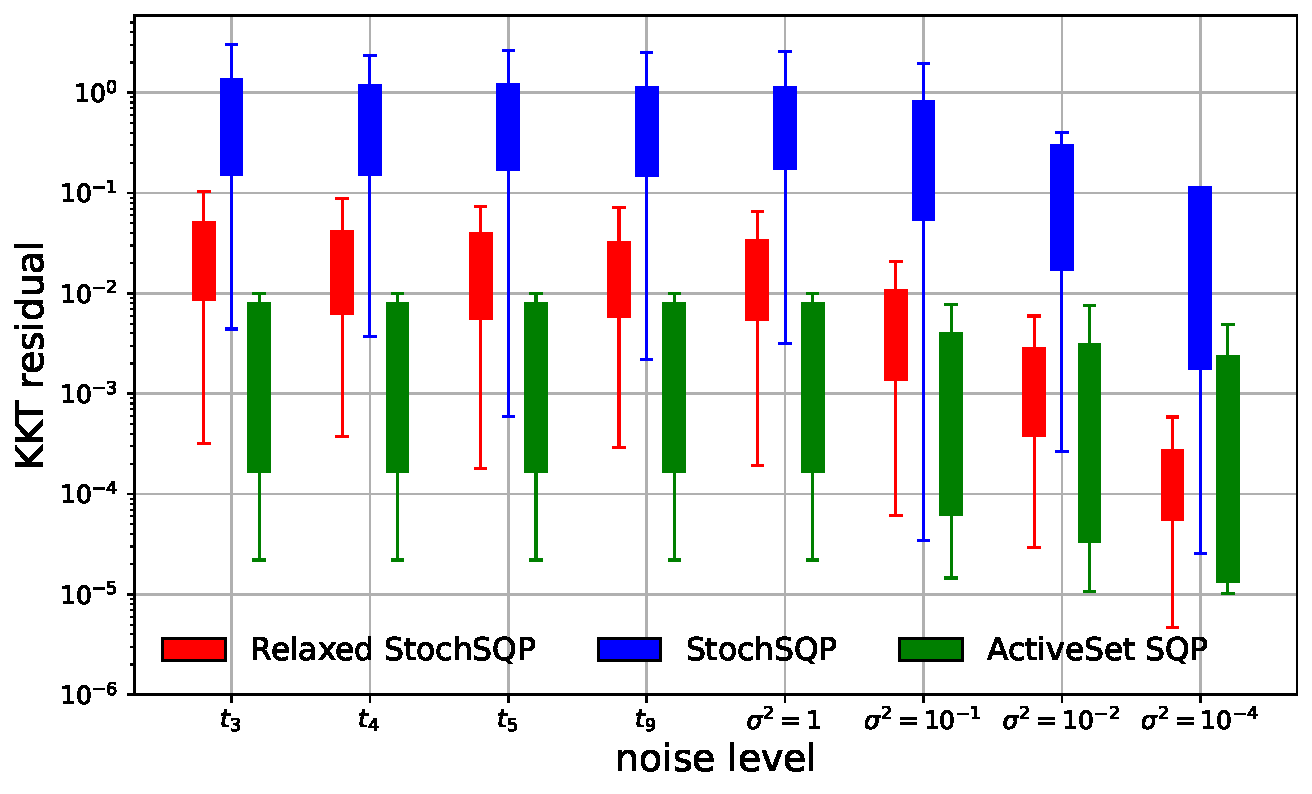
\includegraphics[width=0.45\textwidth]{Figures/box_plot_cutest_kkt.pdf}
    }\  \hspace{0em}
    \subfloat
    [Feasibility errors] 
    {
    \label{fig:cutest_kkt2}     
    %\resizebox{0.28\textwidth}{!}{\input{fig/syn_relu_g_depth.pgf}}
    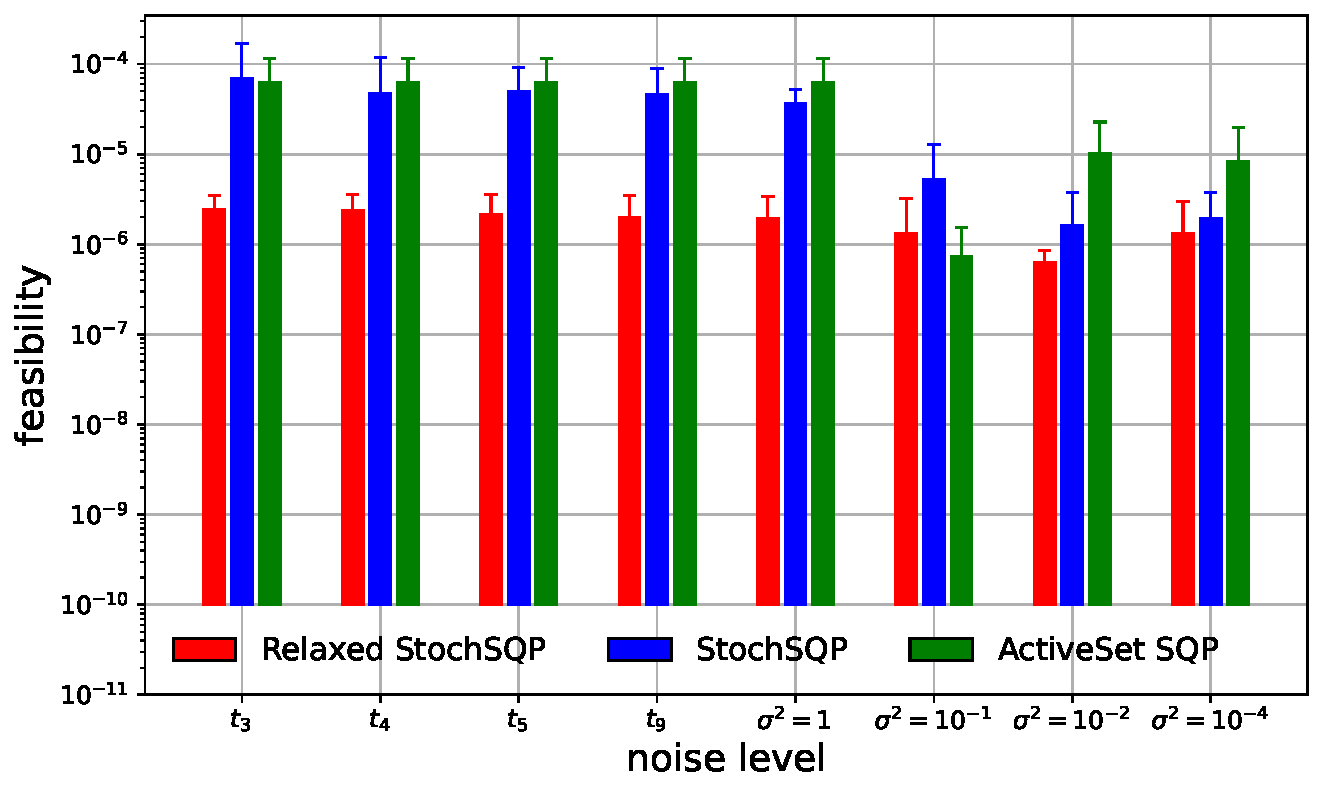
\includegraphics[width=0.45\textwidth]{Figures/box_plot_cutest_feas.pdf}
    }\
    }\\
    \caption{		
	 KKT residuals and feasibility errors of the Relaxed SQP, StochSQP, and ActiveSet SQP on CUTEst problems.}	
    \label{fig:cutest_kkt}
\end{figure}  

\begin{table}[h]
  \centering
  \caption{The coverage rate (Cov Rate) and length of confidence intervals (Avg Len) for some CUTEst (constrained) problems. The standard deviation of the interval length is also reported.}
  \label{tab:cutest_covrate}
  \begin{tabular}{ccccccc}
    \hline
    \multirow{2}{*}{\textbf{Problem}} & \multirow{2}{*}{\textbf{Noise Level}} & \multicolumn{2}{c}{\textbf{Gaussian}} & \multirow{2}{*}{\textbf{Freedom}}  & \multicolumn{2}{c}{\textbf{Student t}} \\
    & & \textbf{Cov Rate}(\%) & \textbf{Avg Len} &  & \textbf{Cov Rate}(\%) & \textbf{Avg Len}\\
    \hline
    \multirow{4}{*}{\textbf{HS41}} & 1E+0 & 97.0 & 2.50E-2 (7.73E-4) & 3 & 86.0 & 3.77E-2 (1.90E-3) \\
    & 1E-1 & 97.5 & 7.59E-3 (7.03E-5) & 4 & 93.0 & 3.06E-2 (1.28E-3) \\
    & 1E-2 & 97.0 & 2.40E-3 (8.69E-6) & 5 & 94.0 & 2.79E-2 (9.25E-4)\\
    & 1E-4 & 97.5 & 2.40E-4 (5.95E-7)& 9 & 97.0 & 2.45E-2 (7.10E-4)\\
    \hline
    \multirow{3}{*}{\textbf{HS65}} & 1E+0 & 94.5 & 1.87E-3 (6.82E-6) & 3 & 96.5 & 3.18E-3 (1.66E-4)\\
    & 1E-1 & 94.5 & 5.92E-4 (1.59E-6) & 4 & 95.0 & 2.59E-3 (1.72E-5)\\
    & 1E-2 & 95.0 & 1.87E-4 (4.96E-7) & 5 & 95.0 & 2.37E-3 (1.11E-5)\\
    & 1E-4 & 94.5 & 1.87E-5 (4.97E-8) & 9 & 94.5 & 2.08E-3 (8.36E-6)\\
    \hline
    \multirow{3}{*}{\textbf{HS68}} & 1E+0 & 97.0 & 2.31E-1 (4.85E-2) & 3 & 95.5 & 3.00E-1 (1.32E-1)\\
    & 1E-1 & 98.0 & 5.09E-2 (2.33E-3) & 4 & 94.5 & 2.08E-1 (6.09E-2) \\
    & 1E-2 & 98.5 & 1.58E-2 (2.23E-4) & 5 & 95.0 & 1.81E-1 (5.07E-2)\\
    & 1E-4 & 95.5 & 1.58E-3 (4.56E-6) & 9 & 94.5 & 1.48E-1 (3.52E-2) \\
    \hline
    \multirow{3}{*}{\textbf{HS71}} & 1E+0 & 97.0 & 1.95E-3 (1.44E-5) & 3 & 94.0 & 3.34E-3 (1.23E-4)\\
    & 1E-1 & 96.5 &  6.17E-4 (1.93E-6) & 4 & 96.0 &  2.74E-3 (6.79E-3)\\
    & 1E-2 & 96.5 & 1.95E-4 (5.20E-7) & 5 & 96.5 & 2.49E-3 (2.51E-5)\\
    & 1E-4 & 98.5 & 1.95E-5 (5.08E-8) & 9 & 95.0 & 2.19E-3 (2.12E-5) \\
    \hline
    \multirow{3}{*}{\textbf{HS81}} & 1E+0 & 94.5 & 3.49E-2 (3.17E-3)  & 3 & 91.0 &  5.04E-2 (7.56E-3)\\
    & 1E-1 & 97.0 & 1.13E-2 (4.77E-5) & 4 & 94.0 & 4.21E-2 (3.51E-3)\\
    & 1E-2 & 98.0 &  3.58E-3 (9.63E-6) & 5 &  94.5 & 3.88E-2 (2.42E-3)\\
    & 1E-4 & 98.0 & 3.59E-4 (9.22E-7) & 9 &  95.0 & 3.43E-2 (2.10E-3) \\
    \hline
  \end{tabular}
\end{table}



\subsection{Constrained regression problems}
We implement our algorithm on constrained regression problems, including both the linear and the logistic regression, as described in section \ref{sec_constrained_regression}. The response $b_k$ is generated based on observations $\bm{a}_k \sim \mathcal{N}\left(\bm{\mu}_{a}, \bm{\Sigma}_{a} \right)$, where the mean vector is set as $\bm{\mu}_a = (1, \cdots, 1, -1, \cdots, -1)$. We explore three different choices of the covariance matrix as in \cite{chen2020statistical}: (i) Identity matrix, i.e., $\bm{\Sigma}_1 = \bm{I}_d$; (ii) Toeplitz matrix, i.e., $(\bm{\Sigma}_{a})_{i,j} = r^{|i-j|}$ for some $r > 0$; (iii) Equicorrelation matrix, i.e., $(\bm{\Sigma}_{a})_{i,j} = r$ for all $i \neq j$ and $(\bm{\Sigma}_{a})_{i,i} = 1$, for some $r > 0$. The true parameter vector of both two regression models is configured as $\bm{x}^{*} = \left( \frac{3}{2d}, \cdots, \frac{3}{2d}, \frac{1}{2d}, \cdots, \frac{1}{2d}\right)^{\top}$. We consider the non-negativity constraints, denoted by $\Omega := \left\{\bm{x}: \bm{1}^{\top} \bm{x} = 1, \bm{x} \geq \bm{0}\right\}$. In the linear regression problem, the noise $\varepsilon_k$ is sampled from $\varepsilon_k \sim \mathcal{N}(0,1)$. We aim to estimate $\hat{\bm{e}}^{\top} \bm{x}^{*}$, where $\hat{\bm{e}} = \left(1,\cdots, 1, -1, \cdots, -1 \right)^{\top}$, by constructing $95\%$ confidence intervals. We report the results in Tables \ref{tab:linear_regression} and \ref{tab:logistic_regression}, highlighting different settings for the Toeplitz matrix and Equicorrelation matrix with $r = 0.4, 0.5, 0.6$ and $r=0.1, 0.2, 0.3$, respectively. In each experiment, we run $200$ times with varying random seeds to calculate the coverage rate (Cov Rate) and the average length (Avg Len) of the confidence interval.
Our results affirm that the constructed $95\%$ confidence intervals closely achieve a $95\%$ coverage rate, therefore, empirically validating our theoretical conclusions on asymptotic normality.
Moreover, we also observe that the average length of confidence intervals are in order of $10^{-2}$, matching the experimental results reported by Chen et al. \cite{chen2020statistical} and Na et al. \cite{na2022asymptotic}. The low standard deviation of these intervals' length relative to their average length suggests robustness across different random seeds. 


\begin{table}[h]
  \centering
  \caption{The coverage rate (Cov Rate) and length of confidence intervals (Avg Len) for constrained linear regression problems. The standard deviation of the interval length is also reported.}
  \label{tab:linear_regression}
  \resizebox{\textwidth}{!}{
  \begin{tabular}{ccccccc}
    \hline
    \textbf{Cov Matrix} & \textbf{Dimension} & \textbf{Cov Rate}(\%) & \textbf{Avg Len} & \textbf{Dimension}  & \textbf{Cov Rate}(\%) & \textbf{Avg Len} \\
    \hline
    \multirow{2}{*}{\textbf{Identity}} & 5 & 93.5 & 3.73E-2 (1.74E-4) &  20 & 92.5 & 4.00E-2 (1.33E-4) \\
    & 10 & 96.5 & 3.91E-2 (1.47E-4) & 30 & 92.5 & 4.03E-2 (1.53E-4)\\
    \hline
    \multirow{2}{*}{\textbf{Toeplitz (0.4)}} & 5 & 94.0 & 3.71E-2 (1.68E-4) & 20 & 96.0 & 3.93E-2 (1.38E-4) \\
     & 10 & 94.5 & 3.82E-2 (1.62E-4) & 30 & 93.0 & 3.98E-2 (1.52E-4) \\
    \hline
    \multirow{2}{*}{\textbf{Toeplitz (0.5)}} & 5 & 94.0 & 3.74E-2 (1.67E-4) & 20 & 96.0 & 3.91E-2 (1.38E-4) \\
    & 10 & 95.5 & 3.82E-2 (1.60E-4)& 30 & 93.0 & 3.95E-2 (1.61E-4) \\
    \hline
    \multirow{2}{*}{\textbf{Toeplitz (0.6)}} & 5 & 94.5 & 3.78E-2 (1.70E-4) &  20 & 96.5 & 3.90E-2 (1.36E-4) \\
      & 10 & 94.5 & 3.83E-2 (1.68E-4) & 30 & 93.5 & 3.94E-2 (1.60E-4) \\
    \hline
    \multirow{2}{*}{\textbf{EquiCorr (0.1)}} & 5 & 93.5 & 3.76E-2 (1.58E-4) &  20 & 94.0 & 4.01E-2 (1.35E-4)\\
     &  10 & 93.0 & 3.92E-2 (1.40E-4) & 30 & 92.5 & 4.05E-2 (1.56E-4) \\
    \hline
    \multirow{2}{*}{\textbf{EquiCorr (0.2)}} & 5 & 92.5 & 3.79E-2 (1.59E-4) &  20 & 93.5 & 4.02E-2 (1.26E-4) \\
     & 10 & 95.0 & 3.94E-2 (1.50E-4)  & 30 & 96.0 & 4.05E-2 (1.44E-4)\\
    \hline
    \multirow{2}{*}{\textbf{EquiCorr (0.3)}} & 5 & 92.5 & 3.83E-2 (1.65E-4) &  20 & 93.0 & 4.03E-2 (1.31E-4) \\
     & 10 & 95.0 & 3.96E-2 (1.46E-4) & 30 & 93.5 & 4.05E-2 (1.49E-4) \\
    \hline
  \end{tabular}
  }
\end{table}



\begin{table}[h]
  \centering
  \caption{The coverage rate (Cov Rate) and length of confidence intervals (Avg Len) for constrained logistic regression problems. The standard deviation of the interval length is also reported.}
  \label{tab:logistic_regression}
\resizebox{\textwidth}{!}{
  \begin{tabular}{ccccccc}
    \hline
    \textbf{Cov Matrix} & \textbf{Dimension} & \textbf{Cov Rate}(\%) & \textbf{Avg Len} & \textbf{Dimension}  & \textbf{Cov Rate}(\%) & \textbf{Avg Len} \\
    \hline
    \multirow{2}{*}{\textbf{Identity}} & 5 & 96.5 & 4.46E-2 (7.97E-5) & 20 & 94.5 & 5.87E-2 (7.13E-5) \\
    & 10 & 94.5 & 5.87E-2 (7.13E-5) & 30 & 93.0 & 7.34E-2 (7.90E-5) \\
    \hline
    \multirow{2}{*}{\textbf{Toeplitz (0.4)}} & 5 & 94.5 & 4.46E-2 (9.06E-5) & 20 & 92.5 & 6.86E-2 (1.01E-4) \\
     & 10 & 95.5 & 5.83E-2 (8.59E-5) & 30 & 93.5 & 7.30E-2 (1.13E-4) \\
    \hline
    \multirow{2}{*}{\textbf{Toeplitz (0.5)}} & 5 & 95.0 & 4.46E-2 (8.91E-5) & 20 & 94.0 & 6.84E-2 (1.08E-4) \\
      & 10 & 94.5 & 5.83E-2 (8.77E-5) & 30 & 93.0 & 7.28E-2 (1.24E-4) \\
    \hline
    \multirow{2}{*}{\textbf{Toeplitz (0.6)}} & 5 & 94.5 & 4.47E-2 (9.63E-5) & 20 & 92.5 & 6.82E-2 (1.19E-4) \\
      & 10 & 94.0 & 5.83E-2 (8.77E-5) & 30 & 94.5 & 7.26E-2 (1.32E-4)\\
    \hline
    \multirow{2}{*}{\textbf{EquiCorr (0.1)}} & 5 & 95.0 & 4.47E-2 (9.22E-5) & 20 & 93.0 & 6.69E-2 (9.40E-5) \\
     & 10 & 94.0 & 5.89E-2 (7.81E-5) & 30 & 93.5 & 7.40E-2 (9.27E-5) \\
    \hline
    \multirow{2}{*}{\textbf{EquiCorr (0.2)}} & 5 & 96.0 & 4.47E-2 (8.86E-4) & 20 & 95.0 & 7.00E-2 (1.05E-4) \\
     & 10 & 95.0 & 5.92E-2 (7.32E-5) & 30 & 92.5 & 7.46E-2 (1.02E-4) \\
    \hline
    \multirow{2}{*}{\textbf{EquiCorr (0.3)}} & 5 & 95.0 & 4.48E-2 (8.59E-5) & 20 & 93.5 & 7.05E-2 (1.09E-4)  \\
     & 10 & 96.0 & 5.95E-2 (7.94E-4) & 30 & 94.5 & 7.52E-2 (1.09E-4) \\
    \hline
  \end{tabular}
  }
\end{table}



\subsection{Portfolio optimization problems}
We investigate portfolio optimization problems using $30$ portfolios selected from the Fama-French 100 Portfolios DataSet, subject to the well-known gross-exposure constraint \cite{fan2012vast}:
$\Omega := \left\{\bm{w}: \bm{1}^{\top} \bm{w} = 1, \left\| \bm{w} \right\|_1 \leq c\right\}$,
where we set $c =3$ and $\bm{w}$ denotes the weights for corresponding stocks. We consider four prevalent portfolio optimization models:
\begin{itemize}
        \item Global minimum variance (GMV)
        \begin{equation*}
            \min_{\bm{w} \in \Omega_c} \bm{w}^{\top} \bm{\Sigma} \bm{w},
        \end{equation*}
        where $\bm{\Sigma}$ is the covariance matrix of target stocks.

        \item Mean-variance (MV)
        \begin{equation*}
            \min_{\bm{w} \in \Omega_c}  -\bm{w}^{\top}\bm{\mu} + \bm{w}^{\top} \bm{\Sigma} \bm{w},
        \end{equation*}
        where $\bm{\mu}$ and $\bm{\Sigma}$ are the mean and the covariance matrix of target stocks.

        \item Exponential utility (EXP)
        \begin{equation*}
            \min_{\bm{w} \in \Omega_c} \mathbb{E} \left[ \exp \left(-\eta \left(\bm{w}^{\top} \bm{a} \right)\right) \right],
        \end{equation*}
        where $\bm{a}$ is the observed price changes and $\eta>0$ is a scaling parameter set to be $\eta= 0.1$ in our experiment.

        \item Logarithmic utility (LOG) $$\min_{\bm{w} \in \Omega_c}  -\mathbb{E} \left[ \log \left( \bm{w}^{\top} \bm{a} + \eta \right)  \right],$$
        where $\bm{a}$ is the observed price changes and $\eta>0$ serves as the regularization parameter to ensure the feasibility of the logarithm.
    \end{itemize}



\begin{table}[h]
  \centering
  \caption{Fama-French 100 Portfolios DataSet, 2021-2023}
\label{tab:portfolio}
\resizebox{0.9\textwidth}{!}{
  \begin{tabular}{ccccc}
    \hline
    \textbf{Model} & \textbf{Return} (\%) & \textbf{Max Drawdown} & \textbf{Sharp Ratio} & \textbf{Sortino Ratio} \\
    \hline
    \textbf{EW} & 15.10 & 0.22 & 0.73 & 1.15 \\
    \textbf{GMV} (ours) & 34.94 & 0.27 & 2.81 & 4.28 \\
    \textbf{GMV} (det) & 33.43 & 0.27 & 2.71 & 4.14 \\
    \textbf{MV} (ours) & 42.21 & 0.28 & 3.36 & 5.09 \\
    \textbf{MV} (det) & 40.31 & 0.28 & 3.29 & 5.02 \\
    \textbf{EXP} (ours) & 52.50 & 0.32 & 2.60 & 3.98 \\
    \textbf{EXP} (det) & 51.85 & 0.31 & 2.55 & 3.86 \\
    \textbf{LOG} (ours) & 54.86 & 0.33 & 2.45 & 3.59 \\
    \textbf{LOG} (det) & 55.08 & 0.32 & 2.46 & 3.57\\
    \hline
    \end{tabular}
  }
\end{table}



The exact mean, covariance, and expectations are inaccessible in practice. Instead, we estimate the stochastic gradient and Hessian of the expected objective using available observations and apply our algorithm to solve the problems. For the portfolio strategy $\bm{w}$, we use historical data from the past year as training samples. 
We assess the performance of our portfolio strategies using four key metrics, calculated over the data from years 2021-2023: the accumulative return, maximum drawdown, sharp ratio, and Sortino ratio. The accumulative return captures the overall gain or loss of the portfolio strategy. The other three are related to the risk of the strategy. The maximum drawdown measures the maximum observed loss from a peak to a trough. The sharp ratio compares the portfolio's return to its risk, taking into account the standard deviation of the portfolio returns. The Sortino ratio is a variation of the sharp ratio, considering the standard deviation of negative portfolio returns. The results are summarized in Table \ref{tab:portfolio}. Interestingly, we observe that the model of logarithmic utility achieves the best accumulative return, consistent with the results reported by \cite{du2023high}. In terms of risk control, however, the mean-variance model is more favorable. We also perform a comparison between our algorithm and the deterministic approach denoted as det. We found that the performance metrics across the two methods are quite similar, suggesting that our algorithm approaches deterministic algorithms because of the use of the averaging gradient and Hessian.



We visualize the weights of two stocks as an example, evaluated by the exponential and the logarithmic utility models, in Figure \ref{fig:portfolio}. The blue line traces the trajectory of the weight corresponding to the stock over time. This is accompanied by a blue band, which represents the estimated standard deviation of the weight, as evaluated by the developed asymptotic normality. The yellow line is the accumulative return of the stock. 
We observe a significant correlation between the weight adjustments and the stock's return trajectory.
Notably, abrupt changes in the stock's return are promptly followed by widened blue bands, indicating a surge in the estimated variance of the weight.
This behavior matches well with intuition and underscores the hypothesis that the variance of the weight may serve as an indicator of the stock's inherent risk.




\begin{figure}[ht]
  \centering
  \subfloat[Stock 1, EXP] {
     \label{exp1}
    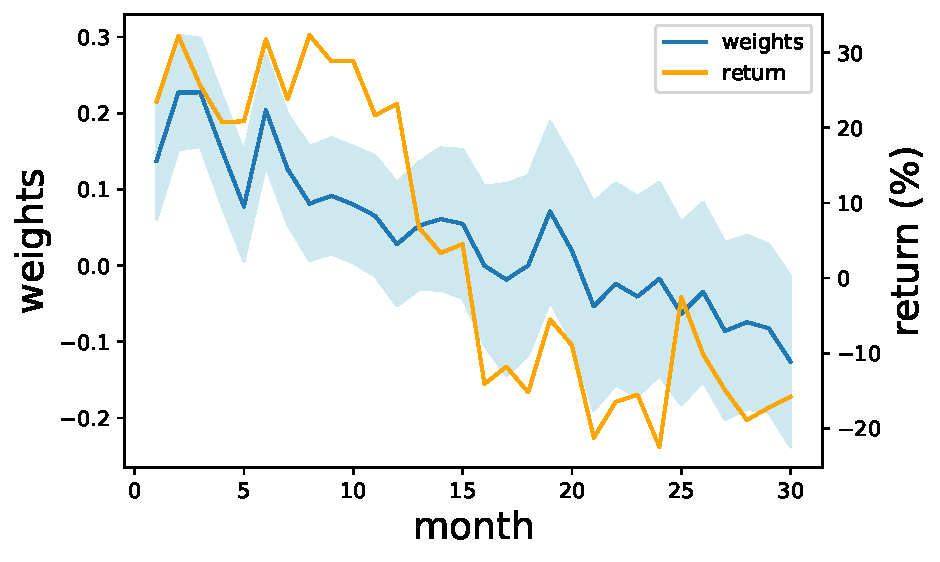
\includegraphics[scale=0.4]{Figures/EXP_1.pdf}
    }\
    \subfloat[Stock 2, EXP]{
    \label{exp2}
    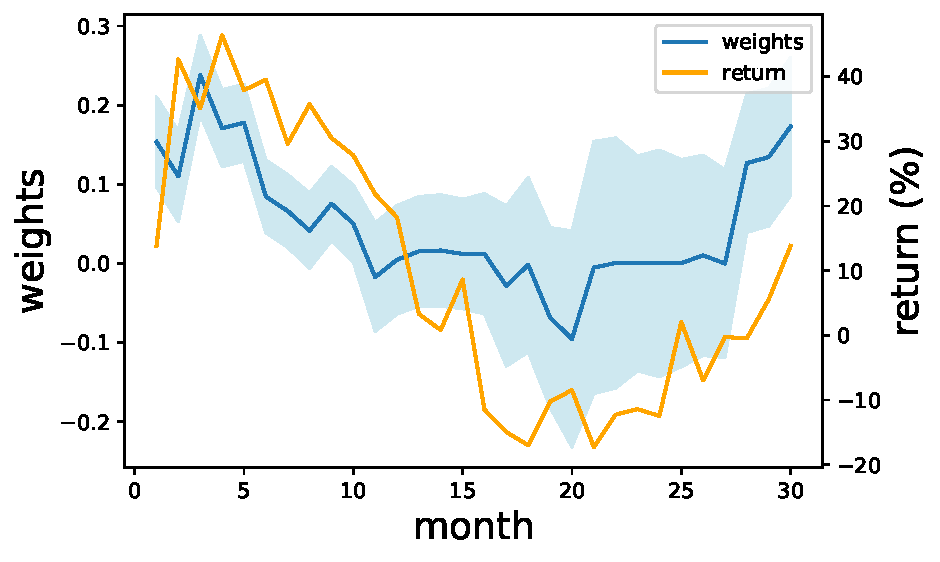
\includegraphics[scale=0.4]{Figures/EXP_2.pdf}
    }\\
  \subfloat[Stock 1, LOG] {
     \label{log1}
    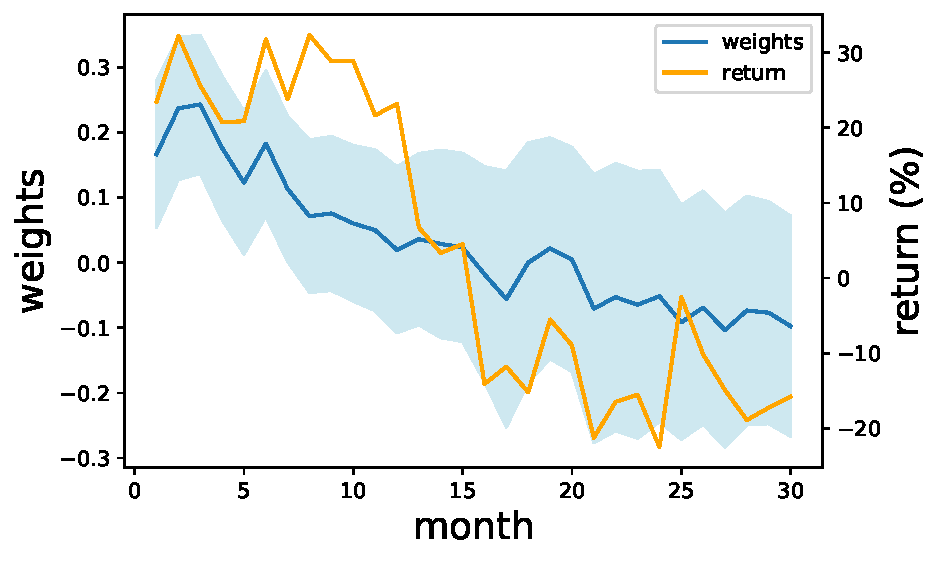
\includegraphics[scale=0.4]{Figures/LOG_1.pdf}
    }\
    \subfloat[Stock 2, LOG]{
    \label{log2}
    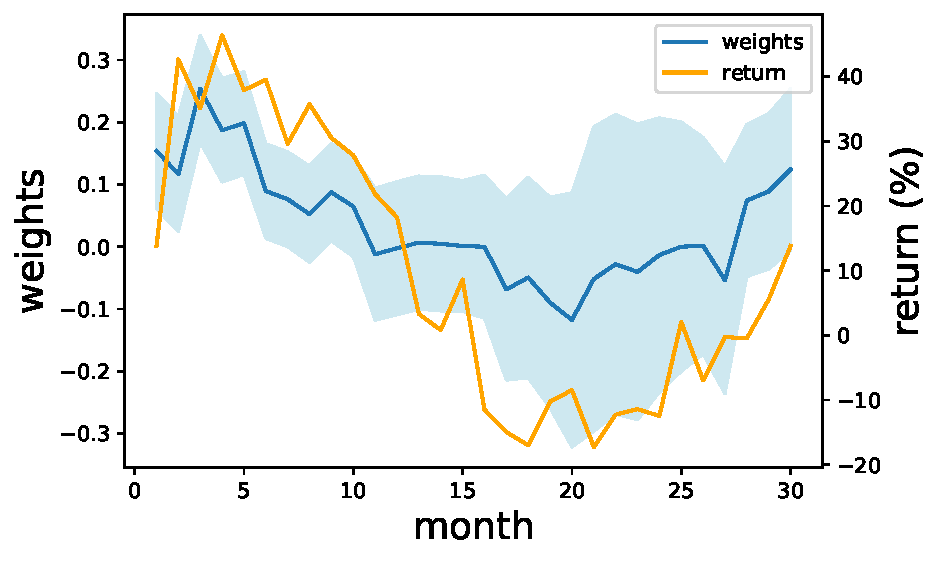
\includegraphics[scale=0.4]{Figures/LOG_2.pdf}
    }\
    \caption{		
	 Weights and returns.}	
    \label{fig:portfolio}
\end{figure}




\subsection{Poisson regression: Chicago air pollution and death rate data}
\label{sec:poisson_regression}
In this section, we study the relationship between different attributes related to air pollution (e.g., PM10, PM25, O3, SO2) and time, with the death rate, by using Poisson regression. 
Let $\bm{a} \in \mathbb{R}^{d}$ represent the vector of air pollution and time attributes, and let $b \in \mathbb{N}$ denote the death rate.
We model the conditional distribution of death $b$ given $\bm{a}$ as a Poisson distribution: $b|\bm{a}  \sim \text{Pois}(\lambda(\bm{a} ))$, where $\log \lambda(\bm{a}) = \bm{a}^{\top} \bm{x}^{*}$ and $\bm{x}^{*}$ is the true, but unknown, parameter vector for the Poisson linear model.
The unconstrained Poisson regression problem is formulated as follows 
    \begin{equation}
    \label{poisson_unconstrained}
            \min_{\bm{x}} \hspace{1em} \mathbb{E} \left[f(\bm{x};\zeta) \right] := \mathbb{E}_{(b,\bm{a})} \left[ b \cdot \bm{a}^{\top} \bm{x} - \exp \left(\bm{a}^{\top} \bm{x} \right) \right].
    \end{equation}
However, based on prior knowledge that air pollution attributes are likely to contribute to an increase in the death rate, we impose non-negativity constraints on the corresponding weights $\bm{x}$.
The constrained Poisson regression model is
\begin{equation}
 \label{poisson_constrained}
        \begin{split}
            \min_{\bm{x}} &  \hspace{1em} \mathbb{E} \left[f(\bm{x};\zeta) \right] := \mathbb{E}_{(b,\bm{a})} \left[ b \cdot \bm{a}^{\top} \bm{x} - \exp \left(\bm{a}^{\top} \bm{x} \right) \right], \\
            \text{s.t.} & \hspace{1em} \bm{x}_{\mathcal{B}} \geq \bm{0},
        \end{split}
    \end{equation}
    where $\mathcal{B}$ is the set of indices of weights corresponding to pollution attributes. 
    Some discussions on the Poisson regression model are included in section \ref{sec_constrained_regression}.


\begin{table}[h]
  \centering
  \caption{Summary of Poisson regression (Model 1) on Chicago air pollution and death rate data}
\label{tab:chicago1}
\resizebox{0.9\textwidth}{!}{
  \begin{tabular}{ccccc}
  \hline
     \textbf{Variables}  & \textbf{Model} & \textbf{Coefficient} ($10^{-2}$) & \textbf{95 \% CI} ($10^{-2}$) & \textbf{p-Value} \\
    \hline
    \multirow{2}{*}{\textbf{PM10}} & \textbf{Model 1} & 0.42 & [-0.57, 1.42] & 0.396 \\
    & \textbf{Ours} & 0.13 & [-0.56,0.79] & 0.371 \\
    \hline
    \multirow{2}{*}{\textbf{PM25}} &  \textbf{Model 1} & 0.72 &  [-0.08, 1.52] & 0.103 \\
    & \textbf{Ours} & 0.65 & [0.02, 1.28] & 0.023 \\
    \hline
    \multirow{2}{*}{\textbf{O3}} & \textbf{Model 1} & -2.97 & [-3.70, -2.24] & 0.000 \\
    & \textbf{Ours}  & 0.00 & active  & \\
    \hline
    \multirow{2}{*}{\textbf{SO2}} & \textbf{Model 1} & 1.38 & [0.58, 2.20] & 0.001 \\
    & \textbf{Ours} & 2.08 & [1.43, 2.73] & 0.000 \\
    \hline
    \multirow{2}{*}{\textbf{Time}} & \textbf{Model 1} & 0.95 & [0.17, 1.74] & 0.008 \\
    & \textbf{Ours} & 1.13 & [0.64, 1.63] & 0.000 \\
    \hline
     \multirow{2}{*}{\textbf{Interc}} & \textbf{Model 1} & 4.6968 & [4.690, 4.704] & 0.000 \\
      & \textbf{Ours} & 4.6974 & [4.692, 4.703] & 0.000\\
      \hline
    \end{tabular}
    }
    \end{table}


\begin{table}[h]
  \centering
  \caption{Summary of Poisson regression (Model 2) on Chicago air pollution and death rate data}
\label{tab:chicago2}
\resizebox{0.9\textwidth}{!}{
  \begin{tabular}{ccccc}
  \hline
     \textbf{Variables}  & \textbf{Model} & \textbf{Coefficient} ($10^{-2}$) & \textbf{95 \% CI} ($10^{-2}$) & \textbf{p-Value} \\
    \hline
    \multirow{2}{*}{\textbf{PM10}} & \textbf{Model 2} &  -0.86 &  [-1.82, 0.10] & 0.062 \\
    & \textbf{Ours} & 0.11 & [-0.52, 0.74] & 0.362 \\
    \hline
    \multirow{2}{*}{\textbf{PM25}} & \textbf{Model 2} & 1.37 & [0.51, 2.23] & 0.001 \\
    & \textbf{Ours} & 0.65 & [0.01, 1.28] & 0.022 \\
    \hline
    \multirow{2}{*}{\textbf{SO2}} & \textbf{Model 2} & 2.06 & [1.28, 2.84] & 0.000 \\
    & \textbf{Ours} & 2.08 & [1.42, 2.73] & 0.000 \\
    \hline 
    \multirow{2}{*}{\textbf{Time}} & \textbf{Model 2} & 1.21 & [0.53, 1.89] & 0.001 \\
    & \textbf{Ours} & 1.13 & [0.64, 1.63] & 0.000 \\
    \hline
     \multirow{2}{*}{\textbf{Interc}} & \textbf{Model 1} & 4.6972 & [4.690, 4.704] & 0.000 \\
      & \textbf{Ours} & 4.6973 & [4.692, 4.703] & 0.000\\
      \hline
    \end{tabular}
    }
    \end{table}


We first consider the unconstrained Poisson regression model (\ref{poisson_unconstrained}), including all five attributes, denoted as Model 1. The estimated model coefficients and their confidence intervals and p-values are provided by the `statsmodels' package in Python \cite{seabold2010statsmodels}. Surprisingly, we observe that the coefficient for O3 is significantly negative, which contradicts our prior understanding of the likely impact of air pollution on death rates. To address this issue, we turn to the constrained Poisson model (\ref{poisson_constrained}), solved by our algorithm. We also estimate the confidence intervals and p-values using the derived asymptotic normality. We list the results in Table \ref{tab:chicago1}. Remarkably, under the non-negativity constraints, the weight of O3 is recognized to be active with the constraints, i.e., it is equal to zero. The estimated model coefficients from the constrained Poisson model are more consistent with our prior beliefs. Next, we consider a reduced model that excludes the O3 attribute, denoted as Model 2. We find that in this model, the weight for PM10 becomes negative, once again contradicting our prior beliefs.
Similarly, employing the constrained Poisson model and solving it via our algorithm, the weight for PM10 becomes positive, although the significance level revealed by the p-value is not particularly strong. The results are reported in Table \ref{tab:chicago2}. 
These findings highlight the importance of incorporating domain-specific constraints in statistical models. They also emphasize the effectiveness of our algorithm in addressing such constrained optimization problems.


\section{Conclusion}
In this work, we proposed a fully stochastic Newton's method for solving constrained optimization problems, called Relaxed StochSQP. We include the averaging technique for both the gradient and Hessian, reducing the impact of stochastic noise and improving the algorithm's performance compared to existing fully stochastic algorithms. We then established the almost sure global convergence in terms of the first-order optimality (KKT) conditions. Furthermore, under certain mild conditions, we developed the asymptotic normality for the proposed algorithm with averaged gradients. It is a particularly surprising and novel result since the gradients in our algorithm are highly correlated. In contrast, previous works primarily rely on the independence of gradients. We also provided a practical plug-in estimator for the covariance matrix. With our results, we are capable of applying Relaxed SQP to perform online inference for constrained optimization problems. 



While our algorithm has demonstrated promising results, there is still potential for further investigation and improvement. Specifically, the current implementation and analysis require the exact solution of quadratic subproblems, which could be computationally expensive. A possible extension of this work would be to explore the use of inexact solutions for the quadratic subproblems. A recent work by Na and Mahoney \cite{na2022asymptotic} employed sketching techniques to inexactly solve linear systems for equality-constrained subproblems. The asymptotic normality behavior still holds for the algorithm with sketching. It remains an open question whether the global almost sure convergence and the local asymptotic normality properties of our algorithm are preserved when fast and inexact solvers are adopted. 
Investigating these areas would help in developing a more efficient and versatile algorithm, with broader applicability in constrained optimization scenarios.


%%%%%%%%%%%%%%%%%%%%%%%%%%%%%%%%%%%%%%%%%%%%%%
%% Single Appendix:                         %%
%%%%%%%%%%%%%%%%%%%%%%%%%%%%%%%%%%%%%%%%%%%%%%
% \begin{appendix}
% \section*{???}%% if no title is needed, leave empty \section*{}.
% \end{appendix}
%%%%%%%%%%%%%%%%%%%%%%%%%%%%%%%%%%%%%%%%%%%%%%
%% Multiple Appendixes:                     %%
%%%%%%%%%%%%%%%%%%%%%%%%%%%%%%%%%%%%%%%%%%%%%%

\begin{appendix}
\newpage
\section{Connections of the Relaxation and EGMFCQ}
\label{sec:appendix1}
\subsection{Proof for Proposition \ref{prop_thetak_to_0}}
\label{sec:appendix1.1}
We first prove the first part of the proposition that the relaxation parameter is non-zero if EGMFCQ holds at the iterate. Define $\mathcal{I}_k := \mathcal{I}(\bm{x}_k):= \{ i \in [d]: (\bm{x}_k)_i = (\bm{\ell})_i \}$ and  $\mathcal{J}_k := \mathcal{J}(\bm{x}_k):= \{ i \in [d]: (\bm{x}_k)_i = (\bm{u})_i \}$, then $\mathcal{I}_k \cap \mathcal{J}_k = \emptyset$ and we denote $\mathcal{A}_k := \mathcal{A}(\bm{x}_k) := \mathcal{I}(\bm{x}_k) \cup \mathcal{J}(\bm{x}_k)$ as the active set of $\bm{x}_k$. Suppose that $\bm{z}_k$ is the vector satisfying (\ref{MFCQ_z}) at $\bm{x}_k$ and we simply let 
$$\varepsilon := \min\left\{\left|(\bm{x}_k - \bm{\ell})_{i}\right|, \left|(\bm{u} -\bm{x}_k)_{i}\right| , \left|(\bm{u} - \bm{\ell})_{j}\right| : i \in \mathcal{A}_k^{-}, j \in \mathcal{A}_k\right\}>0,$$
and
\begin{equation*}
    \Bar{\bm{z}}_k = \frac{\varepsilon}{\|\bm{z}_k\|_2} \bm{z}_k.
\end{equation*}
Then, it is not difficult to verify that 
\begin{equation*}
    \bm{\ell} \leq \bm{x}_k + \Bar{\bm{z}}_k \leq \bm{u},
\end{equation*}
and
\begin{equation}
\label{construct_theta_k}
    \frac{\varepsilon}{\|\bm{z}_k\|_2} \bm{c}(\bm{x}_k) + \nabla \bm{c}(\bm{x}_k) \Bar{\bm{z}}_k = \bm{0},
\end{equation}
which imply that $\Bar{\bm{z}}_k \in \widetilde{\Omega}_k$ with $\theta_k = \frac{\varepsilon}{\|\bm{z}_k\|_2}$. The following lemma shows that if $\widetilde{\Omega}_k$ with $\Bar{\theta} \in (0,1]$ is feasible and $0<\Bar{\Bar{\theta}} \leq \Bar{\theta}$, then $\widetilde{\Omega}_k$ with $\Bar{\Bar{\theta}}$ is also feasible. It further indicates that Assumption \ref{assump1} on the lower-boundedness of the relaxation parameter makes sense. 


\begin{lemma}
\label{prop_reason}
    If $\{\bm{p}: \Bar{\theta} \bm{c}_k +  \bm{J}_k^{\top} \bm{p} = \bm{0}\} \cap \{\bm{p}: \bm{\ell} \leq \bm{x}_k + \bm{p} \leq \bm{u}\} \neq \emptyset$ and $0<\Bar{\Bar{\theta}} \leq \Bar{\theta}$, then $\{\bm{p}: \Bar{\Bar{\theta}} \bm{c}_k +  \bm{J}_k^{\top} \bm{p} = \bm{0}\} \cap \{\bm{p}: \bm{\ell} \leq \bm{x}_k + \bm{p} \leq \bm{u}\} \neq \emptyset$. Therefore, Assumption \ref{assump1} makes sense. 
\end{lemma}


\begin{proof}
    Suppose that $\Bar{\bm{p}} \in \{\bm{p}: \Bar{\theta} \bm{c}_k +  \bm{J}_k^{\top} \bm{p} = \bm{0}\} \cap \{\bm{p}: \bm{\ell} \leq \bm{x}_k + \bm{p} \leq \bm{u}\}$, then $\Bar{\theta} \bm{c}_k +  \bm{J}_k^{\top} \Bar{\bm{p}}  = \bm{0}$ and thus, $\Bar{\Bar{\theta}} \bm{c}_k +  \bm{J}_k^{\top} \left(\Bar{\Bar{\theta}} /\Bar{\theta} \cdot \Bar{\bm{p}}\right)  = \bm{0}$. Let $\Bar{\Bar{\bm{p}}} = \Bar{\Bar{\theta}} /\Bar{\theta} \cdot \Bar{\bm{p}}$, then $\Bar{\Bar{\theta}} \bm{c}_k +  \bm{J}_k^{\top} \Bar{\Bar{\bm{p}}}  = \bm{0}$ and $\bm{\ell} \leq \bm{x}_k + \Bar{\Bar{\bm{p}}} \leq \bm{u}$, which complete the proof.
\end{proof}


\begin{lemma}
[Theorem 3 in \cite{robinson1976stability}]
\label{prop_MFCQ_neighborhood}
    If $\Bar{\bm{x}}$ satisfies EGMFCQ, then there exists a neighborhood $\mathcal{B}(\Bar{\bm{x}};\Bar{r}):= \{\bm{x}: \|\bm{x}- \Bar{\bm{x}}\|_2 \leq \Bar{r}\}$ with some sufficiently small radius $\Bar{r}>0$, such that all points in the neighborhood satisfy EGMFCQ. 
\end{lemma}


\begin{lemma}
\label{prop_continuity_z}
    Suppose that EGMFCQ holds at $\Bar{\bm{x}}$, then EGMFCQ also holds at $\Bar{\bm{x}}_{k}$ when $\Bar{\bm{x}}_{k}$ is sufficiently close to $\Bar{\bm{x}}$, for any sequence $\Bar{\bm{x}}_{k} \to \Bar{\bm{x}}$, by Lemma \ref{prop_MFCQ_neighborhood}. Let $\Bar{\bm{z}}$ be the vectors satisfying (\ref{MFCQ_z}) at $\Bar{\bm{x}}$. Then we can always find a sequence of vectors $\{\Bar{\bm{z}}_{k}\}$ with $\Bar{\bm{z}}_{k}$ satisfying (\ref{MFCQ_z}) at $\Bar{\bm{x}}_{k}$ such that
    $\left\| \Bar{\bm{z}}_{k} - \Bar{\bm{z}} \right\|_2 \to 0$ as $\left\| \Bar{\bm{x}}_{k} - \Bar{\bm{x}} \right\|_2 \to 0$. 
\end{lemma}


\begin{proof}
    Since the vector $\Bar{\bm{z}}$ satisfies (\ref{MFCQ_z}) at $\Bar{\bm{x}}$, i.e., $\bm{c}(\Bar{\bm{x}}) + \nabla \bm{c}(\Bar{\bm{x}})^{\top} \Bar{\bm{z}} = \bm{0}$, by the smoothness of $\bm{c}(\bm{x})$ and the linear independence of columns of $\nabla \bm{c}(\Bar{\bm{x}})$, we can find $\Bar{\bm{z}}_{k}$ such that $\bm{c}(\Bar{\bm{x}}_{k}) + \nabla \bm{c}(\Bar{\bm{x}}_{k})^{\top} \Bar{\bm{z}}_{k} = \bm{0}$ and  $\left\| \Bar{\bm{z}}_{k} - \Bar{\bm{z}}  \right\|_2 \to 0$ as $\left\| \Bar{\bm{x}}_{k}  - \Bar{\bm{x}}  \right\|_2 \to 0$. Let $\varepsilon := \min \{|(\Bar{\bm{z}})_i|: (\Bar{\bm{x}})_{i} = (\bm{\ell})_i~\text{or}~(\Bar{\bm{x}})_{i} = (\bm{u})_i\}$. Due to the fact that $\mathcal{A}(\Bar{\bm{x}}_{k}) \subseteq \mathcal{A}(\Bar{\bm{x}})$, we have $(\Bar{\bm{z}}_{k})_i >0,~\text{if}~(\Bar{\bm{x}}_{k})_{i} = (\bm{\ell})_i$ and $(\Bar{\bm{z}}_{k})_i < 0,~\text{if}~(\Bar{\bm{x}}_{k})_{i} = (\bm{u})_i$, when $\left\| \Bar{\bm{z}}_{k} - \Bar{\bm{z}} \right\|_2 \leq \varepsilon$. 
    
\end{proof}


\begin{lemma}
    Let $\theta_k$ be selected in $(0,1]$ such that the relaxed feasible region $\widetilde{\Omega}_k$ is nonempty with $\theta_k$ but is empty with $\min\{1.1\theta_k,1\}$, and we can always achieve it based on Lemma \ref{prop_reason}. If $\mathop{\lim \inf}_{k \to \infty} \theta_k = 0$, then there exists an accumulation point $\bm{x}^{*}$ of $\{\bm{x}_k\}$ where EGMFCQ does not hold at $\bm{x}^{*}$.
\end{lemma}


\begin{proof}
    Without the loss of generality, we assume that $\lim_{k \to \infty} \theta_k = 0$ and $\lim_{k \to \infty} \bm{x}_k = \bm{x}^{*}$. Let $l_k := \inf \{\|\bm{z}_k\|_2: \bm{z}_k~ \text{satisfies (\ref{MFCQ_z}) at}~ \bm{x}_k\}$. The construction of $\theta_k = \frac{\varepsilon}{\|\bm{z}_k\|_2}$ in (\ref{construct_theta_k}) shows that $\mathop{\lim \sup}_{k \to \infty} l_k = \infty$. Suppose that EGMFCQ holds at $\bm{x}^{*}$ and let $l^{*} = \|\bm{z}^{*}\|_2 < \infty$ for some $\bm{z}^{*}$ satisfying (\ref{MFCQ_z}) at $\bm{x}^{*}$. It is a contradiction to Lemma \ref{prop_continuity_z} as $\infty = \mathop{\lim \sup}_{k \to \infty} l_k \leq l^{*} < \infty$. Therefore, EGMFCQ does not hold at $\bm{x}^{*}$.
\end{proof}


EGMFCQ and its multiple variants are common in constrained optimization algorithms, i.e., \cite{burke1989robust, xu2015smoothing}. According to the above proposition, EGMFCQ makes the relaxed SQP subproblem feasible. Instead of assuming the EGMFCQ at all iterates $\{\bm{x}_k\}$, which is difficult to verify in real applications, a weaker and more explicit assumption (Assumption \ref{assump1}) is made. Proposition \ref{prop_reason} shows the reasonability of Assumption \ref{assump1}. To verify Assumption \ref{assump1}, as shown in the deterministic SQP (Algorithm \ref{alg_det_relaxed_sqp}), we first validate and adopt a feasible $\widetilde{\Omega}_k$ with proper relaxation parameters $\theta_k$. If $\widetilde{\Omega}_k$ is not feasible for small $\theta_k$ below the predefined tolerance, we have reasons to doubt that $\bm{x}_k$ is close to a point where EGMFCQ does not hold, by Lemma \ref{prop_thetak_to_0}. For completeness, we put the definition of LICQ here.

\begin{definition}
    [Linear independence constraint qualification (LICQ)]
    \label{definition_LICQ}
    The linear independence constraint qualification (LICQ) is satisfied at a point $\Tilde{\bm{x}}$, if columns of $[\nabla \bm{c}(\Tilde{\bm{x}}), \bm{I}_{\mathcal{A}(\Tilde{\bm{x}})}]$ are linearly independent, where $\mathcal{A}(\Tilde{\bm{x}}):=\{i: (\Tilde{\bm{x}})_i = (\bm{\ell})_i~\text{or}~(\Tilde{\bm{x}})_i = (\bm{u})_i\}$ is the active set of inequality constraints at $\Tilde{\bm{x}}$.
\end{definition}


\subsection{EGMFCQ and Boundedness of Lagrangian Multipliers}
\label{sec:appendix1.2}
 The following Lemma \ref{lemma_mfcq} shows that if the sequence $\{\bm{x}_k\}$ generated by the algorithm is convergent to a feasible point $\bm{x}^{*}$ satisfying EGMFCQ (Definition \ref{def_MFCQ}), then the corresponding Lagrangian multipliers of the SQP subproblem are bounded. 


 \begin{lemma}
\label{lemma_mfcq}
    If EGMFCQ is satisfied at $\Bar{\bm{x}}$ which is feasible for both the equality and inequality constraints (i.e., $\bm{c}(\Bar{\bm{x}}) = \bm{0}$ and $\bm{\ell} \leq \Bar{\bm{x}} \leq \bm{u}$), then there exists a neighborhood $\mathcal{B}(\Bar{\bm{x}}; r_0):= \{\bm{x}: \|\bm{x} - \Bar{\bm{x}}\|_2 \leq r_0\}$ with some  $r_0>0$, such that the Lagrangian multipliers of the SQP subproblems are bounded for all points in $\mathcal{N}(\Bar{\bm{x}}; r_0)$, under Assumptions \ref{assump1} and \ref{assump2}.  
\end{lemma}

\begin{proof}
    We prove it by contradiction. Suppose that there exist sequences $\{(\Bar{\bm{x}}_k, \Bar{\bm{B}}_k, \Bar{\bm{\lambda}}_{k}^{\text{sub}}, \Bar{\bm{\mu}}_{1,k}^{\text{sub}}, \Bar{\bm{\mu}}_{2,k}^{\text{sub}})\}$ with Assumptions \ref{assump1} and \ref{assump2}, such that 
    $\Bar{\bm{x}}_k \to \Bar{\bm{x}}$, $\left\| (\Bar{\bm{\lambda}}_{k}^{\text{sub}}, \Bar{\bm{\mu}}_{1,k}^{\text{sub}}, \Bar{\bm{\mu}}_{2,k}^{\text{sub}})\right\|_2 \to \infty$ and $\kappa_1 \mathbf{I} \preceq \Bar{\bm{B}}_k \preceq \kappa_2 \mathbf{I}$, where $\Bar{\bm{p}}_k$ and $(\Bar{\bm{\lambda}}_{k}^{\text{sub}}, \Bar{\bm{\mu}}_{1,k}^{\text{sub}}, \Bar{\bm{\mu}}_{2,k}^{\text{sub}})$ are the solution and the Lagrangian multipliers of the SQP subproblem at $\Bar{\bm{x}}_k$ with corresponding relaxing parameters $\Bar{\theta}_k$ satisfying
    \begin{equation}
    \label{KKT_subproblem}
        \begin{split}
            & \nabla f (\Bar{\bm{x}}_k) + \Bar{\bm{B}}_k \Bar{\bm{p}}_k+ \nabla \bm{c}(\Bar{\bm{x}}_k) \Bar{\bm{\lambda}}_{k}^{\text{sub}} - \Bar{\bm{\mu}}_{1,k}^{\text{sub}} + \Bar{\bm{\mu}}_{2,k}^{\text{sub}} = \bm{0},\\
            & \Bar{\theta}_k \bm{c}(\Bar{\bm{x}}_k) + \nabla \bm{c}(\Bar{\bm{x}}_k)^{\top} \Bar{\bm{p}}_k = \bm{0},\quad \bm{\ell} \leq \Bar{\bm{x}}_k + \Bar{\bm{p}}_k \leq \bm{u},\\
            & \Bar{\bm{\mu}}_{1,k}^{\text{sub} \top} (\Bar{\bm{x}}_k + \Bar{\bm{p}}_k - \bm{\ell}) = 0,\\
            & \Bar{\bm{\mu}}_{2,k}^{\text{sub}\top}(\Bar{\bm{x}}_k + \Bar{\bm{p}}_k - \bm{u}) = 0,\\
            & \Bar{\bm{\mu}}_{1,k}^{\text{sub}} \geq \bm{0}, \quad \Bar{\bm{\mu}}_{2,k}^{\text{sub}} \geq \bm{0}.
        \end{split}
    \end{equation}
    Note that the sequence $\{(\Bar{\bm{\lambda}}_{k}^{\text{sub}}, \Bar{\bm{\mu}}_{1,k}^{\text{sub}}, \Bar{\bm{\mu}}_{2,k}^{\text{sub}}) / \left\| (\Bar{\bm{\lambda}}_{k}^{\text{sub}}, \Bar{\bm{\mu}}_{1,k}^{\text{sub}}, \Bar{\bm{\mu}}_{2,k}^{\text{sub}})^{\top}\right\|_2\}$ is bounded. Without the loss of generality, we assume that $(\Bar{\bm{\lambda}}_{k}^{\text{sub}}, \Bar{\bm{\mu}}_{1,k}^{\text{sub}}, \Bar{\bm{\mu}}_{2,k}^{\text{sub}}) / \left\| (\Bar{\bm{\lambda}}_{k}^{\text{sub}}, \Bar{\bm{\mu}}_{1,k}^{\text{sub}}, \Bar{\bm{\mu}}_{2,k}^{\text{sub}})^{\top}\right\|_2 \to (\Bar{\bm{\lambda}}, \Bar{\bm{\mu}}_{1}, \Bar{\bm{\mu}}_{2})$, $\Bar{\bm{p}}_k \to \Bar{\bm{p}}$ and $\Bar{\theta}_k = \Bar{\theta}$ (due to line 4 in Algorithm \ref{alg_det_relaxed_sqp}). Then dividing both two sides of the first equality in  (\ref{KKT_subproblem}) by $\left\| (\Bar{\bm{\lambda}}_{k}, \Bar{\bm{\mu}}_{1,k}, \Bar{\bm{\mu}}_{2,k})^{\top}\right\|_2$ and taking the limit of $k \to \infty$, we have 
    \begin{equation}
    \label{eq17}
        \nabla \bm{c}(\Bar{\bm{x}}) \Bar{\bm{\lambda}} - \Bar{\bm{\mu}}_{1} + \Bar{\bm{\mu}}_{2} = \bm{0}.
    \end{equation}
    Moreover, the second equality in (\ref{KKT_subproblem}) implies that
    \begin{equation*}
        \Bar{\theta} \Bar{\bm{\lambda}}^{\top} \bm{c}(\Bar{\bm{x}}) =  - \Bar{\bm{\lambda}}^{\top} \nabla \bm{c}(\Bar{\bm{x}})^{\top} \Bar{\bm{p}}.
    \end{equation*}
     The third and the fourth equality in (\ref{KKT_subproblem}) further shows that
     \begin{equation*}
         \Bar{\bm{\mu}}_{1}^{\top} (\Bar{\bm{x}} - \bm{\ell}) = -\Bar{\bm{\mu}}_{1}^{\top} \Bar{\bm{p}} \quad \text{and} \quad \Bar{\bm{\mu}}_{2}^{\top} (\Bar{\bm{x}} - \bm{u}) = -\Bar{\bm{\mu}}_{2}^{\top} \Bar{\bm{p}}.
     \end{equation*}
     Combing with the above four equalities, we have
     \begin{equation}
     \label{eq18}
          \Bar{\theta} \Bar{\bm{\lambda}}^{\top} \bm{c}(\Bar{\bm{x}}) + \Bar{\bm{\mu}}_{1}^{\top} (\bm{\ell} - \Bar{\bm{x}}) + \Bar{\bm{\mu}}_{2}^{\top} (\Bar{\bm{x}} - \bm{u}) = 0.
     \end{equation}
     Note that $\Bar{\bm{\mu}}_{1} \geq \bm{0}$ and $\Bar{\bm{\mu}}_{2} \geq \bm{0}$, we can deduce from (\ref{eq18}) and $\bm{c}(\Bar{\bm{x}}) = \bm{0}$ that $(\Bar{\bm{\mu}}_{1}) > 0$ only if $(\Bar{\bm{x}})_{i} = (\bm{\ell})_i$ and $(\Bar{\bm{\mu}}_{2}) > 0$ only if $(\Bar{\bm{x}})_{i} = (\bm{u})_i$. The EGMFCQ condition at $\Bar{\bm{x}}$ (Definition \ref{def_MFCQ}) implies that there exists $\bm{p} \in \mathbb{R}^{d}$ such that $\bm{c}(\Bar{\bm{x}}) + \nabla \bm{c}(\Bar{\bm{x}})^{\top} \bm{p} = \bm{0}$, $(\bm{p})_{i} > 0$ if $(\Bar{\bm{x}})_{i} = (\bm{\ell})_i$, and $(\bm{p})_{i} < 0$ if $(\Bar{\bm{x}})_{i} = (\bm{u})_i$. Then $- \bm{p}^{\top} \Bar{\bm{\mu}}_{1} + \bm{p}^{\top} \Bar{\bm{\mu}}_{2} < 0$ if $\Bar{\bm{x}}$ is on the boundary of the box constraints. 
     Multiplying both two sides of (\ref{eq17}) by $-\Bar{\theta}\bm{p}$, we have $0 = -\Bar{\theta} \bm{p}^{\top}(\nabla \bm{c}(\Bar{\bm{x}}) \Bar{\bm{\lambda}} - \Bar{\bm{\mu}}_{1} + \Bar{\bm{\mu}}_{2}) = \Bar{\theta}\bm{c}(\Bar{\bm{x}})^{\top} \Bar{\bm{\lambda}} + \Bar{\theta} \bm{p}^{\top} \Bar{\bm{\mu}}_{1} - \Bar{\theta} \bm{p}^{\top} \Bar{\bm{\mu}}_{2}$. It is a contradiction to (\ref{eq18}). On the other hand, if $\Bar{\bm{x}}$ is in the interior of the box constraints, $\Bar{\bm{\mu}}_{1} = \Bar{\bm{\mu}}_{2} = \bm{0}$. Together with (\ref{eq17}), the linear independence of the columns of $\nabla \bm{c}(\Bar{\bm{x}})$ shows $\Bar{\bm{\lambda}} = \bm{0}$, which is a contradiction to the fact that $\|(\Bar{\bm{\lambda}}, \Bar{\bm{\mu}}_{1}, \Bar{\bm{\mu}}_{2})^{\top}\|_2 = 1$.
\end{proof}


\begin{corollary}
    If all accumulation points of the sequence $\{\bm{x}_k\}$ are feasible and satisfy EGMFCQ, then the Lagrangian multipliers of the corresponding SQP subproblems are bounded. 
\end{corollary}


\begin{proof}
    We first show that the Lagrangian multipliers of the corresponding SQP subproblems are bounded at all accumulation points of $\{\bm{x}_k\}$, denoted as $\mathcal{X}$. Note that the set $\mathcal{X}$ is closed, any accumulation point of $\mathcal{X}$ is also an accumulation point of $\{\bm{x}_k\}$. 

    Secondly, by Lemma \ref{lemma_mfcq}, for a sufficiently large number $M_{\text{Lag}}>0$ and any point $\bm{x}^{*}_{i} \in \mathcal{X}$, there exists $r_{i}>0$ such that the Lagrangian multipliers of the corresponding SQP subproblems are bounded at $\bm{x}$ for any $\bm{x} \in \cup_{i=1}^{\infty}\mathcal{B}(\bm{x}_{i}^{*};r_i)$. There must be a finite subset of $\{\bm{x}_k\}$, that is outside $\cup_{i=1}^{\infty}\mathcal{B}(\bm{x}_{i}^{*};r_i)$ (otherwise, we can still find an accumulation point). We complete the proof. 
\end{proof}


\subsection{Proof for Theorem \ref{theorem_det_sqp}} 
\label{sec:appendix1.3}
The proof directly comes from the following lemmas. The first lemma here shows that the directional derivative of the merit function is controlled by the improvement $\Delta q(\bm{x},\bm{p},\nabla f(\bm{x}),\bm{B},\rho)$.

\begin{lemma}
 \label{lemma1}
 Under Assumption \ref{assump2}, given $(\bm{x},\rho,\theta,\bm{B},\bm{p}) \in \mathbb{R}^{n} \times \mathbb{R}_{>0} \times (0,1] \times \mathbb{S}_{+}^{n} \times \mathbb{R}^{n}$ with $\theta \bm{c}(\bm{x}) + \nabla \bm{c}(\bm{x})^{\top} \bm{p} = \bm{0}$, then the directional derivative of $\phi(\bm{x},\rho)$ along $\bm{p}$ satisfies
 \begin{equation}
\begin{split}
        \phi^{\prime}(\bm{x},\rho;\bm{p}) & = \nabla f(\bm{x})^{\top} \bm{p} - \rho \theta \|\bm{c}(\bm{x})\|_2 \\
        & \leq \nabla f(\bm{x})^{\top} \bm{p} + \frac{1}{2} \bm{p}^{\top}\bm{B}\bm{p} - \rho \theta \|\bm{c}(\bm{x})\|_2\\
        & = -\Delta q(\bm{x},\bm{p},\nabla f(\bm{x}),\bm{B},\rho).
\end{split}
 \end{equation}
 \end{lemma}

 \begin{proof}
     We prove it by the definition of the directional derivative. Suppose that $\|\nabla^2 f(\bm{x})\|_2 \leq M$ for some $M>0$. First, 
     % without the loss of generality, we assume $\alpha \leq 1$, then  
     \begin{equation}
     \label{eq1}
         \begin{split}
             & \phi(\bm{x}+\alpha \bm{p},\rho) - \phi(\bm{x},\rho) \\
             = & f(\bm{x}+ \alpha \bm{p}) + \rho \|\bm{c}(\bm{x}+\alpha \bm{p})\|_2 - f(\bm{x}) -  \rho \|\bm{c}(\bm{x})\|_2 \\
             \leq & \alpha \nabla f(\bm{x})^{\top} \bm{p} + \frac{\kappa_{\nabla f}}{2} \alpha^2 \|\bm{p}\|_2^2 + \rho \|\bm{c}(\bm{x}+\alpha \bm{p})\|_2 - \rho \|\bm{c}(\bm{x})\|_2\\
             = &  \alpha \nabla f(\bm{x})^{\top} \bm{p} + \frac{\kappa_{\nabla f}}{2} \alpha^2 \|\bm{p}\|_2^2 + \rho \left( \left| 1- \alpha \theta \right| - 1 \right) \|\bm{c}(\bm{x})\|_2 + \frac{\kappa_{\nabla c}}{2}\alpha^2 \|\bm{p}\|_2^2\\
             = & \alpha \left(\nabla f(\bm{x})^{\top} \bm{p} - \rho \theta \|\bm{c}(\bm{x})\|_2 \right) + \frac{\kappa_{\nabla f}+\kappa_{\nabla c}}{2} \alpha^2 \|\bm{p}\|_2^2.
         \end{split}
     \end{equation}
     On the other side, similarly, we have $\phi(\bm{x}+\alpha \bm{p},\rho) - \phi(\bm{x},\rho) \geq \alpha \left(\nabla f(\bm{x})^{\top} \bm{p} - \rho \theta \|\bm{c}(\bm{x})\|_2 \right) - \frac{\kappa_{\nabla f}+\kappa_{\nabla c}}{2} \alpha^2 \|\bm{p}\|_2^2$. Taking limits for $\alpha \to 0$ and the definition, we have $\phi^{\prime}(\bm{x},\rho;\bm{p})  = \nabla f(\bm{x})^{\top} \bm{p} - \rho \theta \|\bm{c}(\bm{x})\|_2 \leq -\Delta q(\bm{x},\bm{p},\nabla f(\bm{x}),\bm{B},\rho)$.
 \end{proof}


We incorporate a backtracking line search in the algorithm while \cite{berahas2021sequential} adopted Lipschitz constant estimation for step size selection. We prove that under mild smoothness conditions, the line search condition will be met after a finite number of search steps. Specifically, the backtracking search loop is guaranteed to terminate within a bounded number of iterations.
 \begin{lemma}
 \label{lemma2}
     The strategies (\ref{det_rho_trial}) and (\ref{det_rho}) for $\rho_k$ guarantee that $\Delta q(\bm{x}_k,\bm{p}_k,\bm{B}_k;\rho_k) \geq \frac{1}{2} \bm{p}_k^{\top} \bm{B}_k \bm{p}_k + \sigma \rho_k \theta_k \|\bm{c}(\bm{x}_k)\|_2$ for some $\sigma \in (0,1)$. Therefore, combining it with Lemma \ref{lemma1}, we have that the backtracking line search condition $\phi(\bm{x}_k+\alpha_k\bm{p}_k,\rho_k) \leq \phi(\bm{x}_k,\rho_k) - \beta \alpha_k \Delta q(\bm{x}_k,\bm{p}_k,\nabla f(\bm{x}_k),\bm{B}_k;\rho_k)$ always holds for $\alpha_k \leq \frac{(1-\beta)\kappa_1}{\kappa_{\nabla f}+\kappa_{\nabla c}}$.
 \end{lemma}

 \begin{proof}
     Equation (\ref{eq1}) in Lemma \ref{lemma1} shows that $\phi(\bm{x}_k+\alpha_k \bm{p}_k,\rho_k) - \phi(\bm{x}_k,\rho_k) \leq \alpha_k \left(\nabla f(\bm{x}_k)^{\top} \bm{p}_k - \rho_k \theta_k \|\bm{c}(\bm{x}_k)\|_2 \right) + \frac{\kappa_{\nabla f}+\kappa_{\nabla c}}{2} \alpha_k^2 \|\bm{p}_k\|_2^2$. Here, we let $\alpha_k$ to be small enough such that  
     \begin{equation*}
         \begin{split}
             &\alpha_k \left(\nabla f(\bm{x}_k)^{\top} \bm{p}_k - \rho_k \theta_k \|\bm{c}(\bm{x}_k)\|_2 \right) + \frac{\kappa_{\nabla f}+\kappa_{\nabla c}}{2} \alpha_k^2 \|\bm{p}_k\|_2^2\\
             \leq &  -\alpha_k \Delta q(\bm{x}_k,\bm{p}_k,\nabla f(\bm{x}_k),\bm{B}_k;\rho_k) + \frac{\kappa_{\nabla f}+\kappa_{\nabla c}}{2} \alpha_k^2 \|\bm{p}_k\|_2^2\\
             \leq & -\beta \alpha_k \Delta q(\bm{x}_k,\bm{p}_k,\nabla f(\bm{x}_k),\bm{B}_k;\rho_k),
         \end{split}
     \end{equation*}
     i.e., $\frac{\kappa_{\nabla f}+\kappa_{\nabla c}}{2} \alpha_k \|\bm{p}_k\|_2^2 \leq (1-\beta)\Delta q(\bm{x}_k,\bm{p}_k,\nabla f(\bm{x}_k),\bm{B}_k;\rho_k)$. Here, we let $\frac{\kappa_{\nabla f}+\kappa_{\nabla c}}{2} \alpha_k \|\bm{p}_k\|_2^2 \leq \frac{(1-\beta) \kappa_1}{2} \|\bm{p}_k\|_2^2 \leq \frac{1-\beta}{2}\bm{p}_k^{\top} \bm{B}_k \bm{p}_k$, i.e., $\alpha_k \leq \frac{(1-\beta)\kappa_1}{\kappa_{\nabla f}+\kappa_{\nabla c}}$. In conclusion, the backtracking line search condition holds when  $\alpha_k \leq \frac{(1-\beta)\kappa_1}{\kappa_{\nabla f}+\kappa_{\nabla c}}$.
 \end{proof}


The next lemma demonstrates that if the Lagrange multipliers are bounded, then the penalty parameter will stabilize. This result is crucial for the global convergence of the algorithm, as convergence is only assured subsequent to the penalty parameter's stabilization. Specifically, once the penalty parameter stabilizes, the merit function's convergence naturally leads to the convergence of the iterates.
\begin{lemma}
  \label{lemma3}
     Under Assumption \ref{assump1}, $\theta_k \geq \Tilde{\tau} \Tilde{\theta}$ holds for all $k=0,1, \cdots$. If we further assume that Assumption \ref{assump2} holds, then the sequence $\{\rho_k\}$ is monotonically increasing and there exists a large enough $\widetilde{K} \in \mathbb{Z}$, such that $\rho_k = \Tilde{\rho} > 0$ for all $k 
     \geq \widetilde{K}$, where $\Tilde{\rho} \leq \frac{(1+\epsilon)M_{\text{Lag}}}{(1-\sigma)\Tilde{\tau} \Tilde{\theta}}$.   
 \end{lemma}

 \begin{proof}
     Under Assumption \ref{assump1}, it is obvious that $\theta_k \geq \Tilde{\tau} \Tilde{\theta}$ holds in our algorithm, for all $k=0,1, \cdots$. If there does not exist $\Tilde{\rho}>0$ and $\widetilde{K} \in \mathbb{Z}$ such that $\rho_k = \Tilde{\rho} > 0$ for $k \geq \widetilde{K}$, according to (\ref{det_rho}), then there is an infinite sequence $\{k_j\} \subseteq \mathbb{Z}_{+}$ where $\rho_{k_j}^{\text{trial}}  > \rho_{k_j-1}$ and $\rho_{k_j} = (1+\epsilon) \rho_{k_j}^{\text{trial}}$. It further implies that $-\nabla f(\bm{x}_k)^{\top} \bm{p}_k - \bm{p}_k^{\top} \bm{B}_k \bm{p}_k < 0$ and $\rho_{k_j}^{\text{trial}} = \frac{\nabla f(\bm{x}_k)^{\top} \bm{p}_k + \bm{p}_k^{\top} \bm{B}_k \bm{p}_k}{(1-\sigma)\theta_k \|\bm{c}(\bm{x}_k)\|_2}$, by (\ref{det_rho_trial}). The KKT conditions for the relaxed SQP subproblem (\ref{relaxed_sqp_subproblem}) show that
     there exist some $(\bm{\lambda}_k^{\text{sub}}, \bm{\mu}_{1,k}^{\text{sub}},\bm{\mu}_{2,k}^{\text{sub}})$ satisfying
     \begin{equation}
     \label{eq6}
         \begin{split}
             & \nabla f(\bm{x}_k) + \bm{B}_k \bm{p}_k + \nabla \bm{c}(\bm{x}_k) \bm{\lambda}_k^{\text{sub}} - \bm{\mu}_{1,k}^{\text{sub}} + \bm{\mu}_{2,k}^{\text{sub}} = \bm{0},\\
             & \theta_k \bm{c}(\bm{x}_{k})+ \nabla \bm{c}(\bm{x}_{k})^{\top}\bm{p}_k = \bm{0},\\
             & \bm{\ell} \leq \bm{x}_k + \bm{p}_k \leq \bm{u},\\
             & \bm{\mu}_{1,k}^{\text{sub} \top}(\bm{x}_k + \bm{p}_k - \bm{\ell}) = 0,\\
             & \bm{\mu}_{2,k}^{\text{sub} \top}(\bm{x}_k + \bm{p}_k - \bm{u}) = 0,\\
             & \bm{\mu}_{1,k}^{\text{sub}} \geq \bm{0}~\text{and}~ \bm{\mu}_{2,k}^{\text{sub}} \geq \bm{0}. 
         \end{split}
     \end{equation}
     Multiplying both two sides of the first equality by $\bm{p}_k$, we have
     \begin{equation*}
     \begin{split}
        \nabla f(\bm{x}_k)^{\top}\bm{p}_k + \bm{p}_k^{\top} \bm{B}_k \bm{p}_k & = -\bm{p}_k^{\top}\nabla \bm{c}(\bm{x}_k) \bm{\lambda}_k^{\text{sub}} + \bm{p}_k^{\top}\bm{\mu}_{1,k}^{\text{sub}} - \bm{p}_k^{\top}\bm{\mu}_{2,k}^{\text{sub}}\\
        & = \theta_k \bm{\lambda}_k^{\text{sub} \top} \bm{c}(\bm{x}_{k}) - \bm{\mu}_{1,k}^{\text{sub} \top}(\bm{x}_k  - \bm{\ell}) + \bm{\mu}_{2,k}^{\text{sub} \top}(\bm{x}_k  - \bm{u})\\
        & \leq \theta_k \bm{\lambda}_k^{\text{sub} \top} \bm{c}(\bm{x}_{k}) \leq \|\bm{\lambda}_k^{\text{sub}}\|_{2} \|\bm{c}(\bm{x}_{k})\|_2 \leq M_{\text{Lag}}\|\bm{c}(\bm{x}_{k})\|_2,
     \end{split}
     \end{equation*}
     where the first inequality comes from $\bm{\mu}_{1,k}^{\text{sub}} \geq \bm{0}$, $\bm{\mu}_{2,k}^{\text{sub}} \geq \bm{0}$, and $\bm{\ell} \leq \bm{x}_k \leq \bm{u}$. Then, 
     \begin{equation}
     \label{eq2}
         \rho_{k_j-1} < \rho_{k_j}^{\text{trial}} = \frac{\nabla f(\bm{x}_{k_j})^{\top} \bm{p}_{k_j} + \bm{p}_{k_j}^{\top} \bm{B}_{k_j} \bm{p}_{k_j}}{(1-\sigma)\theta_{k_j} \|\bm{c}(\bm{x}_{k_j})\|_2} \leq \frac{M_{\text{Lag}}}{(1-\sigma)\theta_{k_j}} \leq \frac{M_{\text{Lag}}}{(1-\sigma)\Tilde{\tau} \Tilde{\theta}}.
     \end{equation}
     However, $\rho_{k_j} = (1+\epsilon) \rho_{k_j}^{\text{trial}} > (1+\epsilon) \rho_{k_j-1}$ implies that $\rho_{k_j-1} \to \infty$ as $k_j \to \infty$. It is a contradiction. Therefore, there exist $\Tilde{\rho}>0$ and a large enough $\widetilde{K} \in \mathbb{Z}$, such that $\rho_k = \Tilde{\rho} > 0$ for all $k 
     \geq \widetilde{K}$. Here, we can also conclude from (\ref{eq2}) that  $\Tilde{\rho} \leq \frac{(1+\epsilon)M_{\text{Lag}}}{(1-\sigma)\Tilde{\tau} \Tilde{\theta}}$.  
 \end{proof}



\begin{proposition}
\label{prop_bound_penalty}
     If we suppose that all accumulation points of the generated sequence $\{\bm{x}_{k}\}$ satisfies EGMFCQ, then $\lim_{k} \rho_k < \infty$. 
 \end{proposition}

 \begin{proof}
     Suppose that $\lim_{k \to \infty} \rho_{k} = \infty$, then we can find a subsequence $\{k_j\} \subseteq \mathbb{Z}_{+}$ such that $\rho_{k_j} > \rho_{k_j - 1}$ and $\rho_k = \rho_{k-1}$ for $k \notin \{k_j\}$. By the fact that 
     \begin{equation*}
         \rho_{k_j}^{\text{trial}} = \frac{\nabla f(\bm{x}_{k_j})^{\top} \bm{p}_{k_j} + \bm{p}_{k_j}^{\top} \bm{B}_{k_j} \bm{p}_{k_j}}{(1-\sigma)\theta_{k_j} \|\bm{c}(\bm{x}_{k_j})\|_2} \leq \frac{M_{\nabla f} M_{\bm{\ell},\bm{u}} + \kappa_2 M_{\bm{\ell},\bm{u}}^2 }{(1-\sigma) \Tilde{\tau} \Tilde{\theta} \|\bm{c}(\bm{x}_{k_j})\|_2},
     \end{equation*}
     we have $\lim_{j \to \infty} \left\| \bm{c}(\bm{x}_{k_j}) \right\|_2 = 0$. By Lemmas \ref{lemma_mfcq} and \ref{lemma3}, it is a contradiction. 
 \end{proof}


Proposition \ref{prop_bound_penalty} shows the boundedness of the penalty parameters from the constraint qualification perspective. More specifically, if EGMFCQ holds for all accumulation points of the sequence $\{\bm{x}_{k}\}$, then the penalty parameter is guaranteed to be bounded. Given that we update the penalty parameter by multiplying it by a factor greater than one, it follows that the penalty parameter will eventually stabilize.

 \begin{lemma}
 \label{lemma4}
     Under Assumptions \ref{assump1} and \ref{assump2}, there exist sufficiently large $\widetilde{K} \in \mathbb{Z}_{+}$ and $\Tilde{\rho}>0$, such that $\rho_k = \Tilde{\rho}$ for all $k \geq \widetilde{K}$ and 
     \begin{equation}
     \label{eq3}
         \phi(\bm{x}_{k},\Tilde{\rho}) - \phi(\bm{x}_{k+1},\Tilde{\rho}) \geq \frac{\beta (1-\beta) \tau\kappa_1 \Tilde{\rho} \Tilde{\tau} \Tilde{\theta} \sigma}{\kappa_{\nabla f}+\kappa_{\nabla c}} \|\bm{c}(\bm{x}_k)\|_2 + \frac{\beta (1-\beta)\kappa_1^2}{2(\kappa_{\nabla f}+\kappa_{\nabla c})} \|\bm{p}_k\|_2^2.
     \end{equation}
 \end{lemma}

 \begin{proof}
     By Lemma \ref{lemma3}, the penalty parameter $\rho_k$ becomes stable when $k \geq \widetilde{K}$ for some sufficiently large $\widetilde{K} \in \mathbb{Z}_{+}$, i.e., $\rho_k = \Tilde{\rho}$ for $k \geq \widetilde{K}$. Next, we only consider the iterates when $\rho_k$ becomes stable. The backtracking line search guarantees that
     \begin{equation*}
        \phi(\bm{x}_{k},\Tilde{\rho}) - \phi(\bm{x}_{k+1},\Tilde{\rho}) \geq  \beta \alpha_k \Delta q(\bm{x}_k,\bm{p}_k, \nabla f(\bm{x}_k),\bm{B}_k,\Tilde{\rho}) \geq \beta \alpha_k \cdot \left(\frac{1}{2} \bm{p}_k^{\top} \bm{B}_k \bm{p}_k + \sigma \Tilde{\rho} \theta_k \|\bm{c}(\bm{x}_k)\|_2\right).
     \end{equation*}
     By Lemma \ref{lemma2}, we have $\alpha_k \geq \frac{\tau (1-\beta)\kappa_1}{\kappa_{\nabla f}+\kappa_{\nabla c}}$ by the backtracking line search. Furthermore, by the positive-definiteness of $\bm{B}_k$ (i.e., $\bm{B}_k \succeq \kappa_1 \mathbf{I}$) and the lower-boundedness of $\theta_k$ (i.e., $\theta_k \geq \Tilde{\tau}\Tilde{\theta}$), together with the stabilization of $\rho_k$ (i.e., $\rho_k = \Tilde{\rho}$) and the lower-boundedness of $\alpha_k$ (i.e., $\alpha_k \geq \frac{\tau (1-\beta)\kappa_1}{\kappa_{\nabla f}+\kappa_{\nabla c}}$), we complete the proof for (\ref{eq3}). 
 \end{proof}


\textbf{Proof for Theorem \ref{theorem_det_sqp}.}
     It is a direct result of Lemma \ref{lemma4}. Here, we only consider the case where the penalty parameter $\rho_k$ becomes stable. By the boundedness of the feasible region (i.e., $\bm{\ell} \leq \bm{x} \leq \bm{u}$) and smoothness of the objective and the constraints, we have that $\phi(\bm{x},\Tilde{\rho})$ is (lower and upper) bounded. Then (\ref{eq3}) implies that
     \begin{equation*}
          \frac{\beta (1-\beta) \tau\kappa_1 \Tilde{\rho} \Tilde{\tau} \Tilde{\theta} \sigma}{\kappa_{\nabla f}+\kappa_{\nabla c}} \sum_{k=\widetilde{K}}^{\infty} \|\bm{c}(\bm{x}_k)\|_2 + \frac{\beta (1-\beta)\kappa_1^2}{2(\kappa_{\nabla f}+\kappa_{\nabla c})} \sum_{k=\widetilde{K}}^{\infty} \|\bm{p}_k\|_2^2 < \infty,
     \end{equation*}
     which completes the proof for (\ref{eq4}). Conditions in (\ref{eq6}) show that $\| \nabla f(\bm{x}_k) +  \nabla \bm{c}(\bm{x}_k) \bm{\lambda}_k^{\text{sub}} - \bm{\mu}_{1,k}^{\text{sub}} + \bm{\mu}_{2,k}^{\text{sub}} \|_2 = \|\bm{B}_k\bm{p}_k\|_2 \leq \kappa_2 \|\bm{p}_k\|_2$, $\|\bm{\mu}_{1,k}^{\text{sub}} \odot (\bm{x}-\bm{\ell})\|_2 \leq \bm{\mu}_{1,k}^{\text{sub} \top}(\bm{x}-\bm{\ell}) \leq M_{\text{Lag}}\|\bm{p}_k\|_2$ and $\|\bm{\mu}_{2,k}^{\text{sub}} \odot (\bm{x}-\bm{u})\|_2 \leq \bm{\mu}_{1,k}^{\text{sub} \top}(\bm{u}-\bm{x}) \leq M_{\text{Lag}}\|\bm{p}_k\|_2$, then (\ref{eq5}) is straightforward.

\subsection{Proof for Lemma \ref{theorem_local_relaxation_parameter}}

Denote $\mathcal{A}^{*} = \mathcal{A}(\bm{x}^{*}):= \{i: (\bm{x}^{*})_i = (\bm{\ell})_i~\text{or}~(\bm{x}^{*})_i = (\bm{\ell})_i\}$ the active set of inequality constraints at $\bm{x}^{*}$. Denote $\varepsilon = \min \{ (\bm{x}^{*}-\bm{\ell})_i, (\bm{u} - \bm{x}^{*})_i, i \in \mathcal{A}^{*-}\} > 0$. First, let $\bm{x}_k$ be sufficiently close to $\bm{x}^{*}$ such that $\|\bm{x}_k - \bm{x}^{*}\|_{\infty} \leq \frac{1}{4} \varepsilon$, then $\min \{ (\bm{x}_{k}-\bm{\ell})_i, (\bm{u} - \bm{x}_{k})_i, i \in \mathcal{A}^{*-}\} \geq \frac{3}{4}\varepsilon$. Since EGMFCQ holds at $\bm{x}^{*}$, there exists a vector $\bm{z}^{*} \in \mathbb{R}^{d}$ satisfying (\ref{MFCQ_z}) at $\bm{x}^{*}$. The fact that $\bm{c}(\bm{x}^{*}) = \bm{0}$ further implies that we can scaling the vector $\bm{z}^{*}$ by some constants such that 
    \begin{equation*}
        \begin{split}
            & \bm{c}(\bm{x}^{*}) + \nabla \bm{c}(\bm{x}^{*})^{\top} \bm{z}^{*} = \bm{0},\\
            & (\bm{z}^{*})_i >0,~\text{if}~(\bm{x}^{*})_{i} = (\bm{\ell})_i,\\
            & (\bm{z}^{*})_i < 0,~\text{if}~(\bm{x}^{*})_{i} = (\bm{u})_i,\\
            & \|\bm{z}^{*}\|_{\infty} \leq \varepsilon/2.
        \end{split}
    \end{equation*}
    By the smoothness of $\bm{c}(\bm{x})$ and the linear independence of columns of $\nabla \bm{c}(\bm{x}^{*})$, we can find $\bm{z}_k$ such that $\bm{c}(\bm{x}_k) + \nabla \bm{c}(\bm{x}_k)^{\top} \bm{z}_k = \bm{0}$ and $\|\bm{z}_k - \bm{z}^{*}\|_{\infty} \leq \frac{1}{2} \min\{|(\bm{z}^{*})_{i}|:(\bm{x}^{*})_{i} = (\bm{\ell})_i ~\text{or}~ (\bm{x}^{*})_{i} = (\bm{u})_i \} \leq \frac{1}{4} \varepsilon$ as $\left\| \bm{x}_k - \bm{x}^{*} \right\|_2 \to 0$. Then $\|\bm{z}_k \|_{\infty} \leq \|\bm{z}_k - \bm{z}^{*}\|_{\infty} + \|\bm{z}^{*}\|_{\infty} \leq \frac{3}{4} \varepsilon$; $(\bm{z}_{k})_i >0,~\text{if}~(\bm{x}^{*})_{i} = (\bm{\ell})_i$ and $(\bm{z}_{k})_i < 0,~\text{if}~(\bm{x}^{*})_{i} = (\bm{u})_i$. Together with the fact that $\min \{ (\bm{x}_{k}-\bm{\ell})_i, (\bm{u} - \bm{x}_{k})_i, i \in \mathcal{A}^{*-}\} \geq \frac{3}{4}\varepsilon$, we show $\bm{\ell} \leq \bm{x}_k + \bm{z}_k  \leq \bm{u}$. Therefore, $\theta_k = 1$ is always accepted if $\bm{x}_k$ is sufficiently close to $\bm{x}^{*}$.


\newpage
\section{Proof for Theorem \ref{theorem_lim_inf} and \ref{theorem_lim}}

\subsection{Some Technical Lemmas for Theorem \ref{theorem_lim_inf}}
We first show that the adaptivity parameter will stabilize after sufficient iterations.
\begin{lemma}
\label{lemma18}
    Under Assumption \ref{assump3}, there exist a constant $\Bar{\xi} > 0$ such that $\xi_k = \Bar{\xi}$ for all sufficiently large $k$.
\end{lemma}

\begin{proof}
    Observe that the sequence $\{\xi_k\}$ is monotonically decreasing and $\xi_{k} < \xi_{k-1}$ holds if and only if $\xi_{k}^{\text{trial}} < \xi_{k-1}$ and $\xi_k \leq (1-\epsilon_{\xi}) \xi_{k-1}$. Suppose $\lim_{k \to \infty} \xi_k = 0$, then it follows that $\mathop{\lim \inf}_{k \to \infty} \xi_k^{\text{trial}} = 0$. However, the selection of $\rho_k$ guarantees that $\Delta q(\bm{x}_k,\Bar{\bm{p}}_k,  \Bar{\bm{g}}_{k},\bm{B}_k,\rho_k) \geq \frac{1}{2} \Bar{\bm{p}}_k^{\top} \bm{B}_k \Bar{\bm{p}}_k \geq \frac{\kappa_1}{2} \|\Bar{\bm{p}}_k\|_2^2$, implying that $\xi_k^{\text{trial}} \geq \frac{\kappa_1}{2}$. It is a contradiction. Therefore, we conclude that $\lim_{k \to \infty} \xi_k > 0$. 
\end{proof}

The following lemma is essential in our subsequent analysis and is extended from Lemma A.3 in \cite{na2022asymptotic}. The results investigate the competition and reveal the asymptotic behavior between the two sequences $\{\alpha_{k}\}$ and $\{\beta_{k}\}$. Importantly, we observe that when $\{\alpha_{k}\}$ decays faster than $\{\beta_{k}\}$, the asymptotic behavior of terms described in the lemma is dominated by the sequence $\{\alpha_{k}\}$, resulting in the asymptotic normality of the generated iterates with averaged gradient as studied in section \ref{sec:asymptotic}. 
\begin{lemma}
    [Lemma A.3 in \cite{na2022asymptotic}]
    \label{lemma_tool}
    For two sequences $\{\alpha_{k}\}$ and $\{\beta_{k}\}$ satisfying $\alpha_k = \iota_1 (k+1)^{-b_1}$ and $\beta_k = \iota_2 (k+1)^{-b_2}$ with $\iota_1, \iota_2 >0$ and $b_1, b_2 > 0$, the followings hold 
    \begin{enumerate}
        \item Define $\chi = 0$ if $0 < b_2 < 1$ and $\chi = -\frac{b_1}{\iota_2}$ if $b_2 = 1$, then
         \begin{equation*}
            \lim_{k \to \infty} \frac{1}{\alpha_k} \sum_{i=0}^{k} \prod_{j=i+1}^{k} \prod_{t = 1}^{l} \left( 1 - a_{t} \beta_{j} \right) \beta_{i} \alpha_{i} =  \frac{1}{\sum_{t=1}^{l} a_t + \chi},
        \end{equation*}
        where we require that $\sum_{t=1}^{l} a_t + \chi> 0$. Moreover,
        \begin{equation*}
            \lim_{k \to \infty} \left\{\frac{1}{\alpha_k} \sum_{i=0}^{k} \prod_{j=i+1}^{k} \prod_{t = 1}^{l} \left( 1 - a_{t} \beta_{j} \right) \beta_{i} \alpha_{i} e_{i} + b \prod_{j=0}^{k} \prod_{t = 1}^{l} \left( 1 - a_{t} \beta_{j} \right) \right\} = 0,
        \end{equation*}
        for any $b \in \mathbb{R}$ and $e_{i} \to 0$.

        \item If $0 < b_2 < b_1 \leq 1$, then 
        \begin{equation*}
            \lim_{k \to \infty} \frac{1}{\alpha_k}  \sum_{i=0}^{k} \prod_{j=i+1}^{k} \left( 1 - \alpha_j \right) \left( 1 - \beta_j \right) \alpha_i \beta_i = 1.
        \end{equation*}
        
    \end{enumerate}
\end{lemma}


\begin{lemma}
\label{lemma20}
    For two given sequence $\{\alpha_k\}$ and $\{\beta_k\}$ satisfying $\lim_{k \to \infty} \alpha_k = 0$, $\lim_{k \to \infty} \beta_k = 0$, and $\lim_{k \to \infty} \alpha_{k}/\beta_k = 0$, then
    \begin{equation}
        \lim_{k \to \infty} \mathbb{E} \left[ \left\| \Bar{\bm{g}}_k - \nabla f(\bm{x}_k)\right\|_2^2 \right] = 0. 
    \end{equation}
    % which implies that $\Bar{\bm{g}}_k - \nabla f(\bm{x}_k) \to 0$ as $k \to \infty$, almost surely.
    Then, there exists a number $M_{\sigma}>0$ such that 
    \begin{equation*}
        \mathbb{E} \left[ \left\| \Bar{\bm{g}}_k - \nabla f(\bm{x}_k)\right\|_2^2 \right] \leq M_{\sigma}^2,
    \end{equation*}
    under Assumption \ref{assump3}.
\end{lemma}


\begin{proof}
By the update scheme of $\Bar{\bm{g}}_{k}$, we have
    \begin{equation*}
        \begin{split}
            \Bar{\bm{g}}_{k} - \nabla f(\bm{x}_k) & = \beta_k \left( \bm{g}_k - \nabla f(\bm{x}_k) \right) + (1-\beta_k) \left( \Bar{\bm{g}}_{k-1} - \nabla f(\bm{x}_{k-1}) \right) \\
            & \hspace{1em} + (1-\beta_k) \left( \nabla f(\bm{x}_{k-1}) - \nabla f(\bm{x}_k) \right)\\
            & = \beta_k \left( \bm{g}_k - \nabla f(\bm{x}_k) \right) + (1-\beta_k)  \left\{ \beta_{k-1} \left( \bm{g}_{k-1} - \nabla f(\bm{x}_{k-1}) \right)  + (1-\beta_{k-1}) \left( \Bar{\bm{g}}_{k-2} - \nabla f(\bm{x}_{k-2}) \right) \right.\\
            & \hspace{1em} + \left. (1-\beta_{k-1}) \left( \nabla f(\bm{x}_{k-2}) - \nabla f(\bm{x}_{k-1}) \right) \right\} + (1-\beta_k) \left( \nabla f(\bm{x}_{k-1}) - \nabla f(\bm{x}_k) \right) \\
            & = \cdots\\
            & = \sum_{i=0}^{k} \left( \prod_{j=i+1}^{k} (1-\beta_j) \right) \beta_i \left( \bm{g}_{i} - \nabla f(\bm{x}_{i}) \right) \\
            & \hspace{1em} + \sum_{i=1}^{k} \left( \prod_{j=i}^{k} (1-\beta_j) \right) \left( \nabla f(\bm{x}_{i-1}) - \nabla f(\bm{x}_{i}) \right) \\
            & := \mathcal{W}_1 + \mathcal{W}_2.
        \end{split}
    \end{equation*}
    Here, both $\mathcal{W}_1$ and $\mathcal{W}_2$ are random variables. Then, $\mathcal{W}_1 - \mathcal{W}_2 \leq \Bar{\bm{g}}_{k} - \nabla f(\bm{x}_k) \leq \mathcal{W}_1 + \mathcal{W}_2$. By Lemma A.3 in [references] and the fact that 
    \begin{equation*}
        \left\|\mathcal{W}_2\right\|_2 \leq \sum_{i=1}^{k} \left( \prod_{j=i}^{k} (1-\beta_j) \right) \alpha_{i-1} M_{\bm{\ell},\bm{u}},
    \end{equation*}
    we have $\mathcal{W}_2 \to 0$ as $k \to \infty$ since $\lim_{k \to \infty} \alpha_{i-1}/\beta_i = 0$. It follows that $\lim_{k \to \infty} \mathbb{E} \left[ \Bar{\bm{g}}_{k} - \nabla f(\bm{x}_k) \right] = \lim_{k \to \infty} \mathbb{E} \left[ \mathcal{W}_1 \right] = 0$. Since
    \begin{equation*}
        \begin{split}
            & \mathbb{E}\left[ \left\|\mathcal{W}_1\right\|_2^2 \right] \\
            = & \sum_{i=0}^{k} \left( \prod_{j=i+1}^{k} (1-\beta_j) \right)^2 \beta_i^2 \mathbb{E}\left[ \left\| \bm{g}_{i} - \nabla f(\bm{x}_{i}) \right\|_2^2 \right] \\
        \leq & \sigma_{g}^2 \sum_{i=0}^{k} \left( \prod_{j=i+1}^{k} (1-\beta_j ) \right)^2 \beta_i^2 \to 0 ~\text{as}~ k \to \infty,
        \end{split}
    \end{equation*}
    where the last convergence result comes from Lemma A.3 in [references]. Therefore,   $\lim_{k \to \infty}\mathbb{E} \left[\left\| \Bar{\bm{g}}_{k} - \nabla f(\bm{x}_k) \right\|_2^2 \right] \leq 2\lim_{k \to \infty}\mathbb{E} \left[ \left\|\mathcal{W}_1\right\|_2^2 \right] + 2 \lim_{k \to \infty} \left\|\mathcal{W}_2\right\|_2^2 = 0$, which completes the first part of the proof. The second result is straightforward since a convergent sequence must be bounded.
\end{proof}


The above lemma establishes the convergence of the averaged gradient to the exact gradient in expectation, by utilizing the asymptotic behavior of two sequences in Lemma \ref{lemma_tool}. The lemma not only assures us of the asymptotic validity of using $\Bar{\bm{g}}_k$ as a surrogate for $\nabla f(\bm{x}_k)$, but also offers a bound for their difference, lending confidence in the effectiveness of the algorithm. Following this, the next lemma studies the perturbation robustness property of the quadratic SQP subproblems and implies that the solutions are Lipschitz continuous with respect to the gradients. Consequently, the fact that the averaged gradient is asymptotically convergent to the exact gradient implies that the proposed algorithm is arbitrarily close to the deterministic algorithm after sufficiently many iterations. This constitutes one of the most significant advantages of our algorithm, employing averaged gradients, over other fully stochastic algorithms \cite{berahas2021sequential, curtis2023sequential}.


\begin{lemma}
\label{lemma19}
    Suppose Assumptions \ref{assump1} , \ref{assump2} and \ref{assump3} hold, then  
    \begin{equation}
        \left\| \Bar{\bm{p}}_k - \bm{p}_k \right\|_2 \leq \kappa_1^{-1} \left\| \Bar{\bm{g}}_{k} - \nabla f(\bm{x}_k)  \right\|_2,
    \end{equation}
    and
    \begin{equation*}
        \mathbb{E}_k \left\| \Bar{\bm{p}}_k - \bm{p}_k \right\|_2 \leq \kappa_1^{-1} \mathbb{E}_k \left\|\Bar{\bm{g}}_{k} - \nabla f(\bm{x}_k)  \right\|_2.
    \end{equation*}
\end{lemma}

\begin{proof}
    The relaxed SQP subproblem at $\bm{x}_k$ with the averaged gradient $\Bar{\bm{g}}_{k}$ can be written as 
    \begin{equation*}
        \min_{\bm{p} \in \widetilde{\Omega}_k} \frac{1}{2}\left\| \bm{p} + \bm{B}_k^{-1} \Bar{\bm{g}}_{k} \right\|_{\bm{B}_k}^2,
    \end{equation*}
    which is a convex-constrained quadratic problem. The variational inequalities [references] imply that 
    \begin{equation*}
        \left \langle \bm{p}_k - \Bar{\bm{p}}_k, - \bm{B}_k^{-1} \Bar{\bm{g}}_{k} - \Bar{\bm{p}}_k \right \rangle_{\bm{B}_k} \leq 0.
    \end{equation*}
    Since $\bm{p}_k$ is the solution of the relaxed SQP subproblem at $\bm{x}_k$ with exact gradient $\nabla f(\bm{x}_k)$, we similarly have 
    \begin{equation*}
        \left \langle  \Bar{\bm{p}}_k - \bm{p}_k, - \bm{B}_k^{-1} \nabla f(\bm{x}_k) - \bm{p}_k \right \rangle_{\bm{B}_k} \leq 0.
    \end{equation*}
    Summing up the above two inequalities, we have 
    \begin{equation}
    \begin{split}
        0 & \geq \left \langle \bm{p}_k - \Bar{\bm{p}}_k, - \bm{B}_k^{-1} \Bar{\bm{g}}_{k} - \Bar{\bm{p}}_k + \bm{B}_k^{-1} \nabla f(\bm{x}_k) + \bm{p}_k\right \rangle_{\bm{B}_k} \\
        & = \left \|  \bm{p}_k - \Bar{\bm{p}}_k \right \|_{\bm{B}_k}^2 + \left \langle  \Bar{\bm{p}}_k - \bm{p}_k, \Bar{\bm{g}}_{k} - \nabla f(\bm{x}_k)  \right \rangle\\
        & \geq \left \|  \bm{p}_k - \Bar{\bm{p}}_k \right \|_{\bm{B}_k}^2 - \left\|  \bm{p}_k - \Bar{\bm{p}}_k\right\|_2 \cdot \left\| \Bar{\bm{g}}_{k} - \nabla f(\bm{x}_k) \right\|_2.
    \end{split}
    \end{equation}
    Note that $\left \|  \bm{p}_k - \Bar{\bm{p}}_k \right \|_{\bm{B}_k}^2 \geq \kappa_1 \left \|  \bm{p}_k - \Bar{\bm{p}}_k \right \|_2^2$, combining with Assumption \ref{assump3}, we complete the proof. 
\end{proof}


\begin{lemma}
\label{lemma21}
    Suppose that Assumptions \ref{assump2} and \ref{assump3} hold, then
    \begin{equation}
        \mathbb{E}_k  \left[ \left|\left( \nabla f(\bm{x}_k) - \Bar{\bm{g}}_{k}\right)^{\top} \Bar{\bm{p}}_k \right|\right] \leq M_{\sigma} M_{\bm{\ell},\bm{u}},
    \end{equation}
    \begin{equation}
        \mathbb{E}_k \left[ \left|\nabla f(\bm{x}_k)^{\top} \bm{p}_k -  \Bar{\bm{g}}_k^{\top} \Bar{\bm{p}}_k \right| \right] \leq M_{\sigma} M_{\bm{\ell},\bm{u}} + 2 \left(M_{\nabla f} + M_{\sigma} \right)  M_{\bm{\ell},\bm{u}},
    \end{equation}
    and
    \begin{equation}
        \mathbb{E}_k\left[ \left|\bm{p}_k^{\top} \bm{B}_k \bm{p}_k -  \Bar{\bm{p}}_k^{\top} \bm{B}_k \Bar{\bm{p}}_k \right| \right] \leq 2\kappa_1^{-1} \kappa_2 M_{\bm{\ell},\bm{u}} M_{\sigma}.
    \end{equation}
\end{lemma}

\begin{proof}
   The first relation is straightforward since $\mathbb{E}_k \left[ \left\| \Bar{\bm{g}}_k - \nabla f(\bm{x}_k)\right\|_2 \right] \leq M_{\sigma}$ and $\|\Bar{\bm{p}}_k\|_2 \leq M_{\bm{\ell},\bm{u}}$. By triangle inequalities, we have
    \begin{equation*}
        \begin{split}
            & \mathbb{E}_k \left[ \left|\nabla f(\bm{x}_k)^{\top} \bm{p}_k -  \Bar{\bm{g}}_k^{\top} \Bar{\bm{p}}_k \right| \right] \\
            = &\mathbb{E}_k \left[ \left| \left( \nabla f(\bm{x}_k) - \Bar{\bm{g}}_k \right)^{\top}\bm{p}_k + \Bar{\bm{g}}_k^{\top} \left(\bm{p}_k - \Bar{\bm{p}}_k \right) \right|\right] \\
            \leq & M_{\sigma} M_{\bm{\ell},\bm{u}} + 2 \left(M_{\nabla f} + M_{\sigma} \right) M_{\bm{\ell},\bm{u}},
        \end{split}
    \end{equation*}
    and
    \begin{equation*}
        \begin{split}
            & \mathbb{E}_k\left[ \left| \bm{p}_k^{\top} \bm{B}_k \bm{p}_k -  \Bar{\bm{p}}_k^{\top} \bm{B}_k \Bar{\bm{p}}_k \right| \right] \\
            = & \mathbb{E}_k\left[ \left|\left(\bm{p}_k - \Bar{\bm{p}}_k\right)^{\top} \bm{B}_k \left(\bm{p}_k + \Bar{\bm{p}}_k \right) \right| \right]\\
            \leq & 2\kappa_2 M_{\bm{\ell},\bm{u}} \mathbb{E}_k\left[ \left\| \bm{p}_k - \Bar{\bm{p}}_k \right\| \right] \leq 2\kappa_1^{-1} \kappa_2 M_{\bm{\ell},\bm{u}} M_{\sigma}.
        \end{split}
    \end{equation*}
\end{proof}


\begin{lemma}
\label{lemma22}
    Suppose that Assumptions \ref{assump1} , \ref{assump2} and \ref{assump3} hold, then
    \begin{equation}
    \begin{split}
        & \mathbb{E}_k \left[ \left|\Delta q(\bm{x}_k,\bm{p}_k,\nabla f(\bm{x}_k),\bm{B}_k;\rho_k) - \Delta q(\bm{x}_k,\Bar{\bm{p}}_k,\Bar{\bm{g}}_{k},\bm{B}_k;\rho_k) \right| \right] \\
        \leq & M_{\sigma} M_{\bm{\ell},\bm{u}} + 2 \left(M_{\nabla f} + M_{\sigma} \right)  M_{\bm{\ell},\bm{u}} + \kappa_1^{-1} \kappa_2 M_{\bm{\ell},\bm{u}} M_{\sigma}.
    \end{split}
    \end{equation}
\end{lemma}

\begin{proof}
    Note that $\Delta q(\bm{x}_k,\bm{p}_k,\nabla f(\bm{x}_k),\bm{B}_k;\rho_k) =  -\nabla f(\bm{x}_k)^{\top} \bm{p}_k - \frac{1}{2} \bm{p}_k^{\top} \bm{B}_k \bm{p}_k + \rho_k \theta_k \|\bm{c}(\bm{x}_k)\|_2$, where the last term $\rho_k \theta_k \|\bm{c}(\bm{x}_k)\|_2$ is independent of $\nabla f(\bm{x}_k)$ and $\bm{p}_k $. Using results in Lemma \ref{lemma21}, we have
    \begin{equation*}
        \begin{split}
            & \mathbb{E}_k \left[ \left| \Delta q(\bm{x}_k,\bm{p}_k,\nabla f(\bm{x}_k),\bm{B}_k;\rho_k) - \Delta q(\bm{x}_k,\Bar{\bm{p}}_k,\Bar{\bm{g}}_{k},\bm{B}_k;\rho_k) \right| \right] \\
            = & \mathbb{E}_k \left[ \left|-\nabla f(\bm{x}_k)^{\top} \bm{p}_k +  \Bar{\bm{g}}_{k}^{\top} \Bar{\bm{p}}_k - \frac{1}{2}\bm{p}_k^{\top} \bm{B}_k \bm{p}_k + \frac{1}{2} \Bar{\bm{p}}_k^{\top} \bm{B}_k \Bar{\bm{p}}_k \right|\right] \\
            \leq & \mathbb{E}_k \left[ \left|-\nabla f(\bm{x}_k)^{\top} \bm{p}_k +  \Bar{\bm{g}}_{k}^{\top} \Bar{\bm{p}}_k  \right| \right] + \frac{1}{2} \mathbb{E}_k \left[ \left| \bm{p}_k^{\top} \bm{B}_k \bm{p}_k -  \Bar{\bm{p}}_k^{\top} \bm{B}_k \Bar{\bm{p}}_k  \right| \right] \\
            \leq & M_{\sigma} M_{\bm{\ell},\bm{u}} + 2 \left(M_{\nabla f} + M_{\sigma} \right)  M_{\bm{\ell},\bm{u}} + \kappa_1^{-1} \kappa_2 M_{\bm{\ell},\bm{u}} M_{\sigma}.
        \end{split}
    \end{equation*}
\end{proof}



\begin{lemma}
\label{lemma23}
    In line 10 of Algorithm \ref{alg_stoch_relaxed_sqp_averaging_grad}, the step size $\alpha_k$ is selected from the interval $[\alpha_k^{\text{min}},\alpha_k^{\text{max}}]:=\left[ \frac{ \xi_{k}\gamma_k}{\kappa_{\nabla f} + \rho_k \kappa_{\nabla c}} , \frac{ \xi_{k}\gamma_k}{\kappa_{\nabla f} + \rho_k \kappa_{\nabla c}} + \varrho \gamma_k^2 \right]$, then 
    \begin{equation}
    \begin{split}
        \mathbb{E}_k \left[ \alpha_k \nabla f(\bm{x}_k)^{\top} \left( \Bar{\bm{p}}_k - \bm{p}_k \right) \right] & \leq \varrho \gamma_k^2 M_{\nabla f} \kappa_1^{-1} M_{\sigma}  + \alpha_k^{\text{min}}  \mathbb{E}_k \left[ \nabla f(\bm{x}_k)^{\top} \left( \Bar{\bm{p}}_k - \bm{p}_k \right)\right],
    \end{split}
    \end{equation}
    under Assumptions \ref{assump2} and \ref{assump3}.
\end{lemma}




\begin{proof}
Denote the event $\mathcal{C}_k = \{\nabla f(\bm{x}_k)^{\top} \left( \Bar{\bm{p}}_k - \bm{p}_k \right) \geq 0\}$, then
    \begin{equation*}
        \begin{split}
             & \mathbb{E}_k \left[ \alpha_k \nabla f(\bm{x}_k)^{\top} \left( \Bar{\bm{p}}_k - \bm{p}_k \right) \right] \\
             = & \mathbb{E}_k \left[ \alpha_k \nabla f(\bm{x}_k)^{\top} \left( \Bar{\bm{p}}_k - \bm{p}_k \right) | \mathcal{C}_{k} \right] + \mathbb{E}_k \left[ \alpha_k \nabla f(\bm{x}_k)^{\top} \left( \Bar{\bm{p}}_k - \bm{p}_k \right) | \mathcal{C}_{k}^{c} \right] \\
             \leq & \alpha_k^{\text{max}}  \mathbb{E}_k \left[  \nabla f(\bm{x}_k)^{\top} \left( \Bar{\bm{p}}_k - \bm{p}_k \right) | \mathcal{C}_{k} \right] +  \alpha_k^{\text{min}}  \mathbb{E}_k \left[  \nabla f(\bm{x}_k)^{\top} \left( \Bar{\bm{p}}_k - \bm{p}_k \right) | \mathcal{C}_{k}^{c} \right] \\
             = & \alpha_k^{\text{min}}  \mathbb{E}_k \left[  \nabla f(\bm{x}_k)^{\top} \left( \Bar{\bm{p}}_k - \bm{p}_k \right)\right] + \left( \alpha_k^{\text{max}}  - \alpha_k^{\text{min}}  \right) \mathbb{E}_k \left[  \nabla f(\bm{x}_k)^{\top} \left( \Bar{\bm{p}}_k - \bm{p}_k \right) | \mathcal{C}_{k} \right] \\
             \leq & \alpha_k^{\text{min}}  \mathbb{E}_k \left[  \nabla f(\bm{x}_k)^{\top} \left( \Bar{\bm{p}}_k - \bm{p}_k \right)\right] + \varrho \gamma_k^2 M_{\nabla f} \kappa_1^{-1} M_{\sigma}.
        \end{split}
    \end{equation*}
\end{proof}



\begin{lemma}
\label{lemma24}
    Under Assumptions \ref{assump1}, \ref{assump2} and \ref{assump3}, if $\sum_{k=0}^{\infty} \gamma_k = \infty$, $\sum_{k=0}^{\infty} \gamma_k^2 < \infty$ and $\sum_{k=\Bar{K}}^{\infty} \alpha_k^{\text{min}} \mathbb{E} \left[\left\|\Bar{\bm{p}}_k - \bm{p}_k \right\|_2\right] < \infty$, then 
        \begin{equation}
        \label{eq25}
        \sum_{k=\Bar{K}}^{\infty}  \alpha_k^{\text{min}} \Delta q(\bm{x}_k,\bm{p}_k,\nabla f(\bm{x}_k),\bm{B}_k;\Bar{\rho}) < \infty,~\text{almost surely}.
    \end{equation}
    It further implies that 
    \begin{equation}
    \label{eq26}
        \mathop{\lim \inf}_{k \to \infty} \Delta q(\bm{x}_k,\bm{p}_k,\nabla f(\bm{x}_k),\bm{B}_k;\Bar{\rho}) = 0,~\text{almost surely}.
    \end{equation}
\end{lemma}


\begin{proof}
    We only consider the case when $\rho_k$ and $\xi_k$ becomes stable, i.e., $\rho_k = \Bar{\rho}$ and $\xi_k = \Bar{\xi}$ for all $k \geq \Bar{K}$. It follows from Assumptions \ref{assump1}, \ref{assump2} and \ref{assump3} that
    \begin{equation}
    \label{eq23}
        \begin{split}
            & \mathbb{E}_k \left[ \phi(\bm{x}_{k+1},\Bar{\rho}) - \phi(\bm{x}_{k},\Bar{\rho}) \right]\\
            = & \mathbb{E}_k \left[ f(\bm{x}_k+\alpha_k \Bar{\bm{p}}_k) - f(\bm{x}_k) + \Bar{\rho}\left(\left\| \bm{c}(\bm{x}_k + \alpha_k \Bar{\bm{p}}_k)\right\|_2 - \left\|\bm{c}(\bm{x}_k) \right\|_2 \right) \right]\\
            \leq & \mathbb{E}_k \left[ \alpha_k \nabla f(\bm{x}_k)^{\top} \Bar{\bm{p}}_{k} + \frac{\kappa_{\nabla f}}{2} \alpha_k^2 \|\Bar{\bm{p}}_k\|_2^2 + \Bar{\rho} \left(\left\| \bm{c}(\bm{x}_k) + \alpha_k \nabla \bm{c}(\bm{x}_k)^{\top} \Bar{\bm{p}}_k)\right\|_2 - \left\|\bm{c}(\bm{x}_k) \right\|_2 + \frac{\kappa_{\nabla c}}{2} \alpha_k^2 \|\Bar{\bm{p}}_k\|_2^2 \right) \right]\\
            = & \mathbb{E}_k \left[ \alpha_k \nabla f(\bm{x}_k)^{\top} \Bar{\bm{p}}_{k} - \alpha_k \Bar{\rho} \theta_k \left\| \bm{c}(\bm{x}_k) \right\|_2 + \frac{\kappa_{\nabla f} + \Bar{\rho} \kappa_{\nabla c}}{2} \alpha_k^2 \|\Bar{\bm{p}}_k\|_2^2  \right]\\
            = & \mathbb{E}_k \left[ \alpha_k \nabla f(\bm{x}_k)^{\top} \bm{p}_{k} + \alpha_k \nabla f(\bm{x}_k)^{\top} \left(\Bar{\bm{p}}_k - \bm{p}_k \right) - \alpha_k \Bar{\rho} \theta_k \left\| \bm{c}(\bm{x}_k) \right\|_2 + \frac{\kappa_{\nabla f} + \Bar{\rho} \kappa_{\nabla c}}{2} \alpha_k^2 \|\Bar{\bm{p}}_k\|_2^2 \right]\\
            = & \mathbb{E}_k \left[-\alpha_k \Delta q(\bm{x}_k,\bm{p}_k,\nabla f(\bm{x}_k),\bm{B}_k,\Bar{\rho}) -\frac{\alpha_k}{2}\bm{p}_k^{\top} \bm{B}_k \bm{p}_k + \alpha_k \nabla f(\bm{x}_k)^{\top} \left(\Bar{\bm{p}}_k - \bm{p}_k \right) + \frac{\kappa_{\nabla f} + \Bar{\rho} \kappa_{\nabla c}}{2} \alpha_k^2 \|\Bar{\bm{p}}_k\|_2^2  \right]\\
            \leq & \mathbb{E}_k \left[ - \alpha_k \Delta q(\bm{x}_k,\bm{p}_k,\nabla f(\bm{x}_k),\bm{B}_k,\Bar{\rho})  -\frac{\alpha_k}{2}\bm{p}_k^{\top} \bm{B}_k \bm{p}_k + \alpha_k \nabla f(\bm{x}_k)^{\top} \left(\Bar{\bm{p}}_k - \bm{p}_k \right) \right. \\
            & \hspace{1em} \left.+ \frac{1}{2} \alpha_k \gamma_k \Delta q(\bm{x}_k,\Bar{\bm{p}}_k,\nabla \Bar{f}(\bm{x}_k),\bm{B}_k,\Bar{\rho})  \right], \\
            = & \mathbb{E}_k \left[ \left( - \alpha_k + \frac{1}{2} \alpha_k \gamma_k \right) \Delta q(\bm{x}_k,\bm{p}_k,\nabla f(\bm{x}_k),\bm{B}_k,\Bar{\rho})  + \alpha_k \nabla f(\bm{x}_k)^{\top} \left(\Bar{\bm{p}}_k - \bm{p}_k \right) \right.\\
            & \hspace{1em} \left.+ \frac{1}{2} \alpha_k \gamma_k \left( \Delta q(\bm{x}_k,\Bar{\bm{p}}_k,\nabla \Bar{f}(\bm{x}_k),\bm{B}_k,\Bar{\rho}) - \Delta q(\bm{x}_k,\bm{p}_k,\nabla f(\bm{x}_k),\bm{B}_k,\Bar{\rho}) \right)  \right], \\
        \end{split}
    \end{equation}
    where the last inequality comes from the selection of $\xi_k$ and $\alpha_k$ in lines 10 and 11, respectively. Without the loss of generality, we assume that $\gamma_k \leq 1$ and continue from (\ref{eq23}), 
    \begin{equation*}
        \begin{split}
            & \mathbb{E}_k \left[ \phi(\bm{x}_{k+1},\Bar{\rho}) - \phi(\bm{x}_{k},\Bar{\rho}) \right] \\
            \leq & \mathbb{E}_k \left[ - \frac{1}{2} \alpha_k^{\text{min}}   \Delta q(\bm{x}_k,\bm{p}_k,\nabla f(\bm{x}_k),\bm{B}_k,\Bar{\rho}) \right] + M_{\nabla f} \alpha_k^{\text{min}} \mathbb{E}_k \left[ \left\|\Bar{\bm{p}}_k - \bm{p}_k \right\|_2 \right] + \varrho \gamma_k^2 M_{\nabla f} \kappa_1^{-1} M_{\sigma}  \\
            & + \frac{1}{2} \alpha_k^{\text{max}} \gamma_k \left( M_{\sigma} M_{\bm{\ell},\bm{u}} + 2 \left(M_{\nabla f} + M_{\sigma} \right) M_{\bm{\ell},\bm{u}} + \kappa_1^{-1} \kappa_2 M_{\bm{\ell},\bm{u}} M_{\sigma} \right),
        \end{split}
    \end{equation*}
    where the inequality is due to Lemmas \ref{lemma22} and \ref{lemma23}. It further implies that 
    \begin{equation}
    \label{eq24}
      \begin{split}
            & \mathbb{E}_k \left[ \phi(\bm{x}_{k+1},\Bar{\rho}) - \min_{\bm{\ell} \leq \bm{x} \leq \bm{u}}\phi(\bm{x},\Bar{\rho}) | \mathcal{F}_{k-1} \right]\\
            \leq & \phi(\bm{x}_{k},\Bar{\rho}) - \min_{\bm{\ell} \leq \bm{x} \leq \bm{u}}\phi(\bm{x},\Bar{\rho}) -\frac{1}{2} \sum_{k=\Bar{K}}^{\Bar{K} + K} \alpha_k^{\text{min}} \mathbb{E}_k \left[ \Delta q(\bm{x}_k,\bm{p}_k,\nabla f(\bm{x}_k),\bm{B}_k,\Bar{\rho}) | \mathcal{F}_{k-1} \right] \\
            &  + M_{\nabla f} \sum_{k=\Bar{K}}^{\Bar{K} + K} \alpha_k^{\text{min}} \mathbb{E}_k \left[ \left\|\Bar{\bm{p}}_k - \bm{p}_k \right\|_2 | \mathcal{F}_{k-1} \right] + \varrho M_{\nabla f} \kappa_1^{-1} M_{\sigma} \sum_{k=\Bar{K}}^{\Bar{K} + K} \gamma_k^2 \\
            &  + \frac{1}{2} \left( M_{\sigma} M_{\bm{\ell},\bm{u}} + 2 \left(M_{\nabla f} + M_{\sigma} \right)  M_{\bm{\ell},\bm{u}} + \kappa_1^{-1} \kappa_2 M_{\bm{\ell},\bm{u}} M_{\sigma} \right) \sum_{k=\Bar{K}}^{\Bar{K} + K}  \alpha_k^{\text{max}} \gamma_k.
      \end{split}
    \end{equation} 
    Since $\sum_{k=0}^{\infty} \gamma_k^2 < \infty$, $\alpha_k^{\text{min}} = \mathcal{O}\left( \gamma_k \right)$ and  $\alpha_k^{\text{max}} = \mathcal{O}\left( \gamma_k + \gamma_k^2 \right)$, we have $\sum_{k=0}^{\infty} \alpha_k^{\text{max}} \gamma_k < \infty$. Note that $\mathbb{E} \left[\sum_{k=\Bar{K}}^{\infty} \alpha_k^{\text{min}} \mathbb{E}_k \left[\left\|\Bar{\bm{p}}_k - \bm{p}_k \right\|_2| \mathcal{F}_{k-1} \right]\right] = \sum_{k=\Bar{K}}^{\infty} \alpha_k^{\text{min}} \mathbb{E} \left[\left\|\Bar{\bm{p}}_k - \bm{p}_k \right\|_2\right] < \infty$ shows that $\sum_{k=\Bar{K}}^{\infty} \alpha_k^{\text{min}} \mathbb{E}_k \left[\left\|\Bar{\bm{p}}_k - \bm{p}_k \right\|_2| \mathcal{F}_{k-1} \right] < \infty$ almost surely. We conclude from (\ref{eq24}), the step size $\alpha_k^{\text{min}} = \mathcal{O}\left( \gamma_k \right)$, the assumption $\sum_{k=\Bar{K}}^{\infty} \alpha_k^{\text{min}} \mathbb{E}_k \left[\left\|\Bar{\bm{p}}_k - \bm{p}_k \right\|_2| \mathcal{F}_{k-1} \right] < \infty$ and Robbins-Siegmund theorem \cite{robbins1971convergence} that (\ref{eq25}) holds. Moreover, since $\sum_{k=0}^{\infty} \gamma_k = \infty$, together with (\ref{eq25}), we obtain (\ref{eq26}).
\end{proof}


\subsection{Proof for Theorem \ref{theorem_lim_inf}}

    Note that although $\{\gamma_k\}$ is the pre-defined sequence in the algorithm, the only difference between $\alpha_k$ and $\gamma_k$ is a constant. Therefore, $\alpha_k^{\text{min}} = \iota_1 (k+1)^{-1}$ implies that $\gamma_k = \iota_3 (k+1)^{-1}$ for some $\iota_3>0$. For simplicity, we directly discuss the behavior of the sequence related to $\alpha_k^{\text{min}}$ rather than $\gamma_k$. We need the techniques and notations in the proof of Lemma \ref{lemma20}, where all conditions are satisfied and $\mathbb{E} \left[\left\| \Bar{\bm{g}}_{k} - \nabla f(\bm{x}_k) \right\|_2^2 \right] \leq 2\mathbb{E} \left[ \left\|\mathcal{W}_1\right\|_2^2 \right] + 2 \mathbb{E} \left[\left\|\mathcal{W}_2\right\|_2^2 \right]$.  In details,
    \begin{equation*}
        \begin{split}
            & \mathbb{E}\left[ \left\|\mathcal{W}_1\right\|_2^2 \right] \\
            = & \sum_{i=0}^{k} \left( \prod_{j=i+1}^{k} (1-\beta_k) \right)^2 \beta_i^2 \mathbb{E}\left[ \left\| \bm{g}_{i} - \nabla f(\bm{x}_{i}) \right\|_2^2 \right] \\
        \leq & \sigma_{g}^2 \sum_{i=0}^{k} \left( \prod_{j=i+1}^{k} (1-\beta_k) \right)^2 \beta_i^2 = \mathcal{O}\left(\beta_k \right),
        \end{split}
    \end{equation*}
    by utilizing Lemma \ref{lemma_tool}.
    Similarly, for $\left\|\mathcal{W}_2\right\|_2$, we have
    \begin{equation*}
        \begin{split}
            & \left\|\mathcal{W}_2\right\|_2 \\
            \leq & M_{\bm{\ell},\bm{u}}  \sum_{i=1}^{k} \left( \prod_{j=i}^{k} (1-\beta_j) \right) \alpha_{i-1}^{\text{min}} = \mathcal{O}\left(\alpha_k^{\text{min}} / \beta_k \right).
        \end{split}
    \end{equation*}
    Therefore, we conclude that $\mathbb{E} \left[\left\| \Bar{\bm{g}}_{k} - \nabla f(\bm{x}_k) \right\|_2 \right] \leq  \mathcal{O}\left(\beta_k + \alpha_k^{\text{min}} / \beta_k \right)$. Since $\alpha_k^{\text{min}} = \iota_1 (k+1)^{-b_1}$, it is not difficult to verify that $\sum_{k=\Bar{K}}^{\infty} \alpha_k^{\text{min}} \mathbb{E} \left[\left\|\Bar{\bm{p}}_k - \bm{p}_k \right\|_2 \right] < \infty$, if $b_1 + \frac{b_2}{2} >1$ and $2b_1 - b_2 >1$. We equivalently require that $b_1 \in (\frac{3}{4},1]$ and $b_2 \in \left( 2-2b_1,2b_1-1\right)$.



    \subsection{Proof for Theorem \ref{theorem_lim}}
We first show that the problem (\ref{est_opt_lagrangian}) is convex and then the corresponding solution $(\bm{\lambda}_{k}^{*}, \bm{\mu}_{1,k}^{*}, \bm{\mu}_{2,k}^{*})$ is well-defined. The stability of quadratic problems in Lemma \ref{lemma13} is an generalization of Lemma \ref{lemma19}.
    \begin{lemma}
    The problem (\ref{est_opt_lagrangian}) is convex, i.e., the Hessian matrix $\nabla^2 F(\bm{\lambda}, \bm{\mu}_{1}, \bm{\mu}_2; \bm{x})$ is positive semi-definite for any $\bm{x}$, $\bm{\lambda}$, $\bm{\mu}_{1}$ and $\bm{\mu}_2$. 
\end{lemma}


\begin{proof}
    The direct computation of the Hessian matrix for $F(\bm{\lambda}, \bm{\mu}_{1}, \bm{\mu}_2; \bm{x})$ is
    \begin{equation}
        \nabla^2 F(\bm{\lambda}, \bm{\mu}_{1}, \bm{\mu}_2; \bm{x}) = \left( \begin{array}{ccc}
            2 \nabla \bm{c}(\bm{x})^{\top} \nabla \bm{c}(\bm{x})  & -2 \nabla \bm{c}(\bm{x}) & 2 \nabla \bm{c}(\bm{x}) \\
            -2 \nabla \bm{c}(\bm{x})^{\top} & 2 \bm{I} + 2 \text{diag}\left( \left( \bm{x} - \bm{\ell} \right)^2 \right) & -2 \bm{I} \\
            2 \nabla \bm{c}(\bm{x})^{\top} & -2 \bm{I} & 2 \bm{I} + 2 \text{diag}\left( \left( \bm{x} - \bm{u} \right)^2 \right) 
        \end{array} \right).
    \end{equation}
    For any vector $\bm{w} = (\bm{w}_1, \bm{w}_2, \bm{w}_3) \in \mathbb{R}^{r} \times \mathbb{R}^{d} \times \mathbb{R}^{d}$,
    \begin{equation*}
        \bm{w}^{\top} \nabla^2 F(\bm{\lambda}, \bm{\mu}_{1}, \bm{\mu}_2; \bm{x}) \bm{w} = \left\| \nabla \bm{c}(\bm{x}) \bm{w}_1 - \bm{w}_2 + \bm{w}_3 \right\|_2^2 + \left\| \left( \bm{x} - \bm{\ell} \right) \odot \bm{w}_2 \right\|_2^2 + \left\| \left( \bm{x} - \bm{u} \right) \odot \bm{w}_3 \right\|_2^2 \geq 0.
    \end{equation*}
    Therefore, the problem (\ref{est_opt_lagrangian}) is convex.
\end{proof}


\begin{lemma}
[Stability of Quadratic Programs, Theorem 2.1 in \cite{daniel1973stability}]
\label{lemma13}
    For two constrained strongly convex quadratic problems 
    \begin{equation*}
        \bm{y}^{*} \in \min_{\bm{y} \in \Lambda} \bm{g}^{\top} \bm{y} + \frac{1}{2} \bm{y}^{\top} \bm{Q} \bm{y},
    \end{equation*}
    and
    \begin{equation*}
        \bm{y}^{**} \in \min_{\bm{y} \in \Lambda} \bm{g}^{\prime \top} \bm{y} + \frac{1}{2} \bm{y}^{\top} \bm{Q}^{\prime} \bm{y},
    \end{equation*}
    where the feasible region $\Lambda$ is convex. Suppose that $\max \{\left\| \bm{y}^{*} \right\|_2, \left\| \bm{y}^{**} \right\|_2 \} \leq M_{y}$ for some $M_{y}>0$. If $\epsilon = \max\{\left\| \bm{g} - \bm{g}^{\prime} \right\|_2, \left\|  \bm{Q} - \bm{Q}^{\prime} \right\|_2 \}$ and both two matrices $\bm{Q}, \bm{Q}^{\prime}$ are positive definite with $\upsilon_1 \bm{I} \preceq \bm{Q}, \bm{Q}^{\prime} \preceq \upsilon_2 \bm{I}$, for some $0<\upsilon_1 \leq \upsilon_2 $. Then, the following holds
    \begin{equation*}
        \left\|\bm{y}^{*} - \bm{y}^{**}  \right\|_2 \leq \epsilon \upsilon_1^{-1} \left( 1 + M_{y} \right). 
    \end{equation*}
\end{lemma}

\begin{lemma}
\label{lemma_lim_kkt}
Under assumptions in Theorem \ref{theorem_lim}, we have 
    \begin{equation*}
        \lim_{k \to \infty} F(\bm{\lambda}_{k}^{*}, \bm{\mu}_{1,k}^{*}, \bm{\mu}_{2,k}^{*}; \bm{x}_k) = 0,~\text{almost surely}.
    \end{equation*}
\end{lemma}


\begin{proof}
    Denote $(\bm{\lambda}_{k}^{\text{sub}}, \bm{\mu}_{1,k}^{\text{sub}}, \bm{\mu}_{2,k}^{\text{sub}})$ as Lagrangian multipliers of the relaxed SQP subproblem at $\bm{x}_k$ with full gradient $\nabla f(\bm{x}_k)$. It follows that
    \begin{equation*}
        \begin{split}
            F(\bm{\lambda}_{k}^{*}, \bm{\mu}_{1,k}^{*}, \bm{\mu}_{2,k}^{*}; \bm{x}_k) & \leq F(\bm{\lambda}_{k}^{\text{sub}}, \bm{\mu}_{1,k}^{\text{sub}}, \bm{\mu}_{2,k}^{\text{sub}}; \bm{x}_k) \leq \left\| \bm{B}_k \bm{p}_k \right\|_2^2 + \left\| \bm{\mu}_{1,k}^{\text{sub}} \odot \bm{p}_k \right\|_2^2 + \left\| \bm{\mu}_{2,k}^{\text{sub}} \odot \bm{p}_k \right\|_2^2 \\
            & \leq (\kappa_2 + 2 M_{\text{Lag}}) \left\| \bm{p}_k \right\|_2^2,
        \end{split}
    \end{equation*}
    then 
    \begin{equation*}
        \mathop{\lim \inf}_{k \to \infty}  F(\bm{\lambda}_{k}^{*}, \bm{\mu}_{1,k}^{*}, \bm{\mu}_{2,k}^{*}; \bm{x}_k)  = 0,
    \end{equation*}
    by $\mathop{\lim \inf}_{k \to \infty} \left\| \bm{p}_k \right\|_2 = 0$. Suppose that $\mathop{\lim \sup}_{k \to \infty}  F(\bm{\lambda}_{k}^{*}, \bm{\mu}_{1,k}^{*}, \bm{\mu}_{2,k}^{*}; \bm{x}_k)  > 0$, we can find a sufficiently small number $\varepsilon >0$ and two infinite sequences $\{m_i\}$ and $\{n_i\}$ with $\Bar{K} \leq m_i < n_i$, such that
    \begin{equation*}
        F(\bm{\lambda}_{m_i}^{*}, \bm{\mu}_{1,m_i}^{*}, \bm{\mu}_{2,m_i}^{*}; \bm{x}_{m_i}) > 2 \varepsilon, \quad \left\| \bm{p}_{n_i} \right\|_2 \leq \sqrt{\frac{\varepsilon}{\kappa_2 + M_{\text{Lag}} }},
    \end{equation*}
    and
    \begin{equation*}
        \left\| \bm{p}_{k} \right\|_2 \geq \sqrt{\frac{\varepsilon}{\kappa_2 + M_{\text{Lag}} }},~\text{for}~m_i \leq k < n_i.
    \end{equation*}
    Note that we can always achieve it due to the following derivation
    \begin{equation}
        \begin{split}
            F(\bm{\lambda}_{k}^{*}, \bm{\mu}_{1,k}^{*}, \bm{\mu}_{2,k}^{*}; \bm{x}_{k}) & = \min_{\bm{\lambda}, \bm{\mu}_{1} \geq \bm{0}, \bm{\mu}_{2} \geq \bm{0}} F(\bm{\lambda}, \bm{\mu}_{1}, \bm{\mu}_2; \bm{x}_k) \\
            & \leq \min_{\bm{\lambda}, \bm{\mu}_{1} \geq \bm{0}, \bm{\mu}_{2} \geq \bm{0}} \left\{F(\bm{\lambda}, \bm{\mu}_{1}, \bm{\mu}_2; \bm{x}_k) + \frac{\varepsilon}{6 M_{\text{Lag}}^2 } \left\|(\bm{\lambda}, \bm{\mu}_{1}, \bm{\mu}_2) \right\|_2^2 \right\} \\
            & \leq F(\bm{\lambda}_{k}^{\text{sub}}, \bm{\mu}_{1,k}^{\text{sub}}, \bm{\mu}_{2,k}^{\text{sub}}; \bm{x}_k) + \frac{\varepsilon}{6 M_{\text{Lag}}^2 } \left\|(\bm{\lambda}_{k}^{\text{sub}}, \bm{\mu}_{1,k}^{\text{sub}}, \bm{\mu}_{2,k}^{\text{sub}}) \right\|_2^2 \\
            & \leq \left\| \bm{B}_k \bm{p}_k \right\|_2^2 + \left\| \bm{\mu}_{1,k}^{\text{sub}} \odot \bm{p}_k \right\|_2^2 + \left\| \bm{\mu}_{2,k}^{\text{sub}} \odot \bm{p}_k \right\|_2^2 + \frac{\varepsilon}{2}\\
            & \leq (\kappa_2 + 2 M_{\text{Lag}}) \left\| \bm{p}_k \right\|_2^2 + \frac{\varepsilon}{2}.
        \end{split}
    \end{equation}
    Here, $F(\bm{\lambda}_{m_i}^{*}, \bm{\mu}_{1,m_i}^{*}, \bm{\mu}_{2,m_i}^{*}; \bm{x}_{m_i}) > 2 \varepsilon$ automatically implies that $\left\| \bm{p}_{m_i} \right\|_2 \geq \sqrt{\frac{3\varepsilon}{2(\kappa_2 + M_{\text{Lag}}) }}$. Since $\mathop{\lim \inf}_{k \to \infty} \left\| \bm{p}_k \right\|_2 = 0$, there must exists $n_i > m_i$ such that $\left\| \bm{p}_{n_i} \right\|_2 \leq \sqrt{\frac{\varepsilon}{\kappa_2 + M_{\text{Lag}} }}$.
    Let
    \begin{equation*}
        \widetilde{F}(\bm{\lambda}, \bm{\mu}_{1}, \bm{\mu}_2; \bm{x}) = F(\bm{\lambda}, \bm{\mu}_{1}, \bm{\mu}_2; \bm{x}_k) + \frac{\varepsilon}{6 M_{\text{Lag}}^2 } \left\|(\bm{\lambda}, \bm{\mu}_{1}, \bm{\mu}_2) \right\|_2^2.
    \end{equation*}
    It also implies that $\widetilde{F}(\bm{\lambda}_{m_i}^{**}, \bm{\mu}_{1,m_i}^{**}, \bm{\mu}_{2,m_i}^{**}; \bm{x}_{m_i}) \geq 2 \varepsilon$ and $ \widetilde{F}(\bm{\lambda}_{n_i}^{**}, \bm{\mu}_{1,n_i}^{**}, \bm{\mu}_{2,n_i}^{**}; \bm{x}_{n_i}) \leq (\kappa_2 + 2 M_{\text{Lag}}) \left\| \bm{p}_{n_i} \right\|_2^2 + \frac{\varepsilon}{2} \leq \frac{3}{2} \varepsilon$, where $(\bm{\lambda}_{m_i}^{**}, \bm{\mu}_{1,m_i}^{**}, \bm{\mu}_{2,m_i}^{**}) \in \min_{\bm{\lambda}, \bm{\mu}_{1} \geq \bm{0}, \bm{\mu}_{2} \geq \bm{0}} \widetilde{F}(\bm{\lambda}, \bm{\mu}_{1}, \bm{\mu}_2; \bm{x}_{m_i})$ and $(\bm{\lambda}_{n_i}^{**}, \bm{\mu}_{1,n_i}^{**}, \bm{\mu}_{2,n_i}^{**}) \in \min_{\bm{\lambda}, \bm{\mu}_{1} \geq \bm{0}, \bm{\mu}_{2} \geq \bm{0}} \widetilde{F}(\bm{\lambda}, \bm{\mu}_{1}, \bm{\mu}_2; \bm{x}_{n_i})$. Note that the function $\widetilde{F}(\bm{\lambda}, \bm{\mu}_{1}, \bm{\mu}_2; \bm{x})$ is strictly positive-definite with
    \begin{equation*}
        \frac{\varepsilon}{6 M_{\text{Lag}}^2 } \leq \left\| \nabla^2 \widetilde{F}(\bm{\lambda}, \bm{\mu}_{1}, \bm{\mu}_2; \bm{x}) \right\|_2 \leq 2\left( M_{\nabla c}^{2} + 4 M_{\nabla c}^{2} + 2 M_{\bm{\ell},\bm{u}}^{2} + 4\right).
    \end{equation*}
    For simplicity, we denote $\bm{w}_k = (\bm{\lambda}_{k}^{**}, \bm{\mu}_{1,k}^{**}, \bm{\mu}_{2,k}^{**})$, then 
    \begin{equation*}
        \frac{\varepsilon}{6 M_{\text{Lag}}^2 } \left\|\bm{w}_k \right\|_2^2 \leq \min_{\bm{\lambda}, \bm{\mu}_{1} \geq \bm{0}, \bm{\mu}_{2} \geq \bm{0}}  \widetilde{F}(\bm{\lambda}, \bm{\mu}_{1}, \bm{\mu}_2; \bm{x}) \leq (\kappa_2 + 2 M_{\text{Lag}}) \left\| \bm{p}_k \right\|_2^2 + \frac{\varepsilon}{2},
    \end{equation*}
    and thus 
    \begin{equation}
    \label{eq22}
        \left\|\bm{w}_k \right\|_2 \leq \sqrt{\frac{6 M_{\text{Lag}}^2 \left( \kappa_2 + 2 M_{\text{Lag}} \right) M_{\bm{\ell},\bm{u}}^{2} }{\varepsilon}} + 3 M_{\text{Lag}},
    \end{equation}
    for all $k \in \mathbb{N}$. 


    We first write $\widetilde{F}(\bm{\lambda}, \bm{\mu}_{1}, \bm{\mu}_2; \bm{x}_k)$ into the general quadratic form that
    \begin{equation*}
        \widetilde{F}(\bm{\lambda}, \bm{\mu}_{1}, \bm{\mu}_2; \bm{x}_{k}) = \left\| \nabla f(\bm{x}_{k}) \right\|_2^2 +  \bm{q}_{k}^{\top} \bm{w} + \frac{1}{2} \bm{w}^{\top} \bm{Q}_{k} \bm{w},
    \end{equation*}
    where
    \begin{equation*}
        \bm{q}_{k} = \left( \begin{array}{c}
             2 \nabla \bm{c}(\bm{x}_{k})^{\top} \nabla f(\bm{x}_{k})   \\
             -2  \nabla f(\bm{x}_{k}) \\
             2 \nabla f(\bm{x}_{k}) 
        \end{array} \right)
    \end{equation*}
    and
    \begin{equation*}
        \bm{Q}_{k} = \left( \begin{array}{ccc}
            2 \nabla \bm{c}(\bm{x}_{k})^{\top} \nabla \bm{c}(\bm{x}_{k})  & -2 \nabla \bm{c}(\bm{x}_{k}) & 2 \nabla \bm{c}(\bm{x}_{k}) \\
            -2 \nabla \bm{c}(\bm{x}_{k})^{\top} & 2 \bm{I} + 2 \text{diag}\left( \left( \bm{x}_{k} - \bm{\ell} \right)^2 \right) & -2 \bm{I} \\
            2 \nabla \bm{c}(\bm{x}_{k})^{\top} & -2 \bm{I} & 2 \bm{I} + 2 \text{diag}\left( \left( \bm{x}_{k} - \bm{u} \right)^2 \right) 
        \end{array} \right) + \frac{\varepsilon}{6 M_{\text{Lag}}^2 } \bm{I}.
    \end{equation*}
    The smoothness of the objective $f(\bm{x})$ and the constraints $\bm{c}(\bm{x})$ show that
    \begin{equation}
    \label{eq20}
        \begin{split}
            \left\| \bm{q}_{k+1} - \bm{q}_{k} \right\|_2 & \leq 2 \left( \kappa_{\nabla c} M_{\nabla f} + M_{\nabla c} \kappa_{\nabla f} + 2 \kappa_{\nabla f} \right) \left\| \bm{x}_{k+1} - \bm{x}_{k} \right\|_2 \\
            & \leq  2 \left( \kappa_{\nabla c} M_{\nabla f} + M_{\nabla c} \kappa_{\nabla f} + 2 \kappa_{\nabla f} \right) M_{\bm{\ell},\bm{u}} \alpha_k,
        \end{split}
    \end{equation}
    and
    \begin{equation}
    \label{eq21}
        \begin{split}
            \left\| \bm{Q}_{k+1} - \bm{Q}_{k} \right\|_2 & \leq 4 \left( M_{\nabla c} \kappa_{\nabla c} + 2 \kappa_{\nabla c} + 2 M_{\bm{\ell},\bm{u}} \right) \left\| \bm{x}_{k+1} - \bm{x}_{k} \right\|_2\\
            & \leq 4 \left( M_{\nabla c} \kappa_{\nabla c} + 2 \kappa_{\nabla c} + 2 M_{\bm{\ell},\bm{u}} \right) M_{\bm{\ell},\bm{u}} \alpha_k.
        \end{split}
    \end{equation}
    Then 
    \begin{equation*}
        \begin{split}
            & \left|  \widetilde{F}(\bm{\lambda}_{k+1}^{**}, \bm{\mu}_{1,k+1}^{**}, \bm{\mu}_{2,k+1}^{**}; \bm{x}_{k+1}) -  \widetilde{F}(\bm{\lambda}_{k}^{**}, \bm{\mu}_{1,k}^{**}, \bm{\mu}_{2,k}^{**}; \bm{x}_{k}) \right| \\
            \leq & \left| \bm{q}_{k+1}^{\top} \bm{w}_{k+1} + \frac{1}{2} \bm{w}^{\top}_{k+1} \bm{Q}_{k+1} \bm{w}_{k+1} - \bm{q}_{k}^{\top} \bm{w}_{k} - \frac{1}{2} \bm{w}^{\top}_{k} \bm{Q}_{k} \bm{w}_{k} \right| + \left| \left\| \nabla f(\bm{x}_{k+1}) \right\|_2^2 - \left\| \nabla f(\bm{x}_{k}) \right\|_2^2 \right|\\
            \leq & \left| \bm{q}_{k+1}^{\top} \bm{w}_{k+1} + \frac{1}{2} \bm{w}^{\top}_{k+1} \bm{Q}_{k+1} \bm{w}_{k+1} - \bm{q}_{k}^{\top} \bm{w}_{k+1} - \frac{1}{2} \bm{w}^{\top}_{k+1} \bm{Q}_{k} \bm{w}_{k+1} \right|\\
            & - \left| \bm{q}_{k}^{\top} \bm{w}_{k+1} + \frac{1}{2} \bm{w}^{\top}_{k+1} \bm{Q}_{k} \bm{w}_{k+1} - \bm{q}_{k}^{\top} \bm{w}_{k} - \frac{1}{2} \bm{w}^{\top}_{k} \bm{Q}_{k} \bm{w}_{k} \right| + \left| \left\| \nabla f(\bm{x}_{k+1}) \right\|_2^2 - \left\| \nabla f(\bm{x}_{k}) \right\|_2^2 \right|\\
            \leq & \left\|\bm{w}_{k+1} \right\|_2 \left\| \bm{q}_{k+1} - \bm{q}_{k} \right\|_2  + \frac{1}{2} \left\| \bm{w}_{k+1} \right\|_2^2 \left\| \bm{Q}_{k+1} - \bm{Q}_{k} \right\|_2 \\
            & + \left\| \bm{q}_{k} \right\|_2 \left\| \bm{w}_{k+1} - \bm{w}_{k} \right\|_2 + \frac{1}{2} \left\| \bm{w}_{k+1} \right\|_2  \left\| \bm{Q}_{k} \right\|_2  \left\| \bm{w}_{k+1} - \bm{w}_{k} \right\|_2 \\
            & + \frac{1}{2} \left\| \bm{w}_{k} \right\|_2 \left\| \bm{Q}_{k} \right\|_2 \left\| \bm{w}_{k+1} - \bm{w}_{k} \right\|_2 +  \left\| \nabla f(\bm{x}_{k+1}) - \nabla f(\bm{x}_{k}) \right\|_2    \left( \left\| \nabla f(\bm{x}_{k+1}) \right\|_2  + \left\| \nabla f(\bm{x}_{k}) \right\|_2\right).
        \end{split}
    \end{equation*}
    Using Lemma \ref{lemma13}, equations (\ref{eq22}), (\ref{eq20}) and (\ref{eq21}), and $\bm{Q}_{k} \succeq \frac{\varepsilon}{ 6 M_{\text{Lag}}^2} \bm{I}$, we have $\left\| \bm{w}_{k+1} - \bm{w}_{k} \right\|_2 = \mathcal{O}\left( \frac{\alpha_k}{\varepsilon^{3/2}} \right)$, where we omit some universal and uncritical constants. Combining it with equations (\ref{eq22}), (\ref{eq20}) and (\ref{eq21}), we have 
    \begin{equation*}
        \left|  \widetilde{F}(\bm{\lambda}_{k+1}^{**}, \bm{\mu}_{1,k+1}^{**}, \bm{\mu}_{2,k+1}^{**}; \bm{x}_{k+1}) -  \widetilde{F}(\bm{\lambda}_{k}^{**}, \bm{\mu}_{1,k}^{**}, \bm{\mu}_{2,k}^{**}; \bm{x}_{k}) \right| \leq M_{F} \frac{\alpha_k}{\varepsilon^2},
    \end{equation*}
    for a universal constant $M_{F}$, which is independent of $\alpha_k$, $k$ and $\varepsilon$.
    
    
    Therefore, it follows from the above inequalities and our construction of the sequences $\{m_i\}$ and $\{n_i\}$ that
    \begin{equation}
        \begin{split}
            \frac{1}{2} \varepsilon & \leq \widetilde{F}(\bm{\lambda}_{m_i}^{*}, \bm{\mu}_{1,m_i}^{*}, \bm{\mu}_{2,m_i}^{*}; \bm{x}_{m_i}) - \widetilde{F}(\bm{\lambda}_{n_i}^{*}, \bm{\mu}_{1,n_i}^{*}, \bm{\mu}_{2,n_i}^{*}; \bm{x}_{n_i}) \\
            & \leq \sum_{k=m_i}^{n_i -1} \left |\widetilde{F}(\bm{\lambda}_{k}^{*}, \bm{\mu}_{1,k}^{*}, \bm{\mu}_{2,k}^{*}; \bm{x}_{k}) - \widetilde{F}(\bm{\lambda}_{k+1}^{*}, \bm{\mu}_{1,k}^{*}, \bm{\mu}_{2,k}^{*}; \bm{x}_{k}) \right| \\
            & \leq \sum_{k=m_i}^{n_i -1} M_{F}  \frac{\alpha_k}{ \varepsilon^2}.
        \end{split}
    \end{equation}
    Summing up both two side from $i=1$ to $\infty$, we have 
    \begin{equation*}
         \infty = \sum_{i=1}^{\infty} \frac{1}{2 M_{F}} \varepsilon^3 \leq  \sum_{i=1}^{\infty} \sum_{k=m_i}^{n_i -1} \alpha_k.
    \end{equation*}
    However, $\left\| \bm{p}_{k} \right\|_2 \geq \sqrt{\frac{\varepsilon}{\kappa_2 + M_{\text{Lag}} }}$ for $m_i \leq k \leq n_i-1$, which further implies that 
    \begin{equation*}
         \sum_{i=1}^{\infty} \sum_{k=m_i}^{n_i -1}  \alpha_k  \leq \frac{ \kappa_2 + M_{\text{Lag}} }{\varepsilon } \sum_{i=1}^{\infty} \sum_{k=m_i}^{n_i -1} \alpha_k  \left\| \bm{p}_{k} \right\|_2^2 \leq \frac{ \kappa_2 + M_{\text{Lag}} }{\varepsilon } \sum_{k=\Bar{K}}^{\infty} \alpha_k  \left\| \bm{p}_{k} \right\|_2^2 < \infty.
    \end{equation*}
    It is a contradiction. Therefore, we complete the proof that $\lim_{k \to \infty} F(\bm{\lambda}_{k}^{*}, \bm{\mu}_{1,k}^{*}, \bm{\mu}_{2,k}^{*}; \bm{x}_k) = 0$.
\end{proof}



\begin{lemma}
\label{lemma_lim_constraints}
Under assumptions in Theorem \ref{theorem_lim}, we have 
     \begin{equation*}
        \lim_{k \to \infty} \bm{c}(\bm{x}_k) = \bm{0},~\text{almost surely}.
    \end{equation*}
\end{lemma}


\begin{proof}
    The proof scheme is similar. For completeness, we provide the details here. Suppose that $\mathop{\lim \sup}_{k \to \infty} \left\| \bm{c}(\bm{x}_k) \right\|_2 = 0$ but $\mathop{\lim \inf}_{k \to \infty} \left\| \bm{c}(\bm{x}_k) \right\|_2 = 0$. Then we can find a sufficiently small number $\varepsilon > 0$ and two infinite sequences $\{m_i\}$ and $\{n_i\}$ with $\Bar{K} \leq m_i < n_i$, such that 
    \begin{equation*}
        \left\| \bm{c}(\bm{x}_{m_i}) \right\|_2 > 2 \varepsilon, \quad \left\| \bm{c}(\bm{x}_{n_i}) \right\|_2 < \varepsilon,
    \end{equation*}
    and
    \begin{equation*}
        \left\| \bm{c}(\bm{x}_k) \right\|_2 \geq \varepsilon,~\text{for}~m_i \leq k < n_i.
    \end{equation*}
    It follows from the definition of the sequence that 
    \begin{equation*}
        \begin{split}
            \varepsilon & \leq \left\| \bm{c}(\bm{x}_{m_i}) \right\|_2 - \left\| \bm{c}(\bm{x}_{n_i}) \right\|_2 \\
            & \leq \sum_{k=m_i}^{n_i-1} \left\| \bm{c}(\bm{x}_{k}) \right\|_2 - \left\| \bm{c}(\bm{x}_{k+1}) \right\|_2 \\
            & \leq \sum_{k=m_i}^{n_i-1}   \left\| \bm{c}(\bm{x}_{k}) - \bm{c}(\bm{x}_{k+1}) \right\|_2  \\
            & \leq \kappa_{c} M_{\bm{\ell},\bm{u}} \sum_{k=m_i}^{n_i-1} \alpha_{k}, \quad \text{for all}~i \in \mathbb{N}.
        \end{split}
    \end{equation*}
    Multiplying both two sides by $\varepsilon$ and by the fact that $\left\| \bm{c}(\bm{x}_k) \right\|_2 \geq \varepsilon,~\text{for}~m_i \leq k < n_i$, we have
    \begin{equation*}
        \varepsilon^2 \leq \kappa_{c} M_{\bm{\ell},\bm{u}} \sum_{k=m_i}^{n_i-1} \alpha_{k} \left\| \bm{c}(\bm{x}_k) \right\|_2 , \quad \text{for all}~i \in \mathbb{N},
    \end{equation*}
    which implies that $\infty \leq \sum_{i=1}^{\infty} \sum_{k=m_i}^{n_i-1} \alpha_{k} \left\| \bm{c}(\bm{x}_k) \right\|_2 \leq \sum_{k=\Bar{K}}^{\infty} \alpha_{k} \left\| \bm{c}(\bm{x}_k) \right\|_2 < \infty$. It is a contradiction.
\end{proof}

Combining with Lemmas \ref{lemma_lim_kkt} and \ref{lemma_lim_constraints}, we finish the proof for Theorem \ref{theorem_lim}.


\newpage
\section{Proof for Theorem \ref{theorem_asymptotic_almost_sure}}
\subsection{Proof for Lemma \ref{lemma_almost_eq}}
We proceed by prove each of the four conclusions in turn. 

\subsubsection{Proof for Conclusion 1} 
% By Theorem \ref{theorem_local_relaxing_parameter}, the unit relaxing parameter $\theta_{k} = 1$ is always accepted when $\bm{x}_{k}$ is sufficiently close to $\bm{x}^{*}$. 
Note that 
    \begin{equation*}
            \bm{p}_{k} \in \mathop{\arg \min}_{\bm{p} \in \Omega_{k}} \nabla f(\bm{x}_{k})^{\top} \bm{p} + \frac{1}{2} \bm{p}^{\top} \bm{B}_{k} \bm{p},
    \end{equation*}
    where $\Omega_k = \{\bm{p}: \bm{c}(\bm{x}_k)+\nabla \bm{c}(\bm{x}_k)^{\top}\bm{p} = \bm{0}\} \cap \{\bm{p}: \bm{\ell} \leq \bm{x}_k + \bm{p} \leq \bm{u}\} $, and let
    \begin{equation*}
        \bm{p}^{*} \in \mathop{\arg \min}_{\bm{p} \in \Omega^{*}} \nabla f(\bm{x}^{*})^{\top} \bm{p} + \frac{1}{2} \bm{p}^{\top} \bm{B}_{k} \bm{p},
    \end{equation*}
    and
    \begin{equation*}
        \bm{p}_{k}^{*} \in \mathop{\arg \min}_{\bm{p} \in \Omega^{*}} \nabla f(\bm{x}_{k})^{\top} \bm{p} + \frac{1}{2} \bm{p}^{\top} \bm{B}_{k} \bm{p},
    \end{equation*}
    where $\Omega^{*} = \{\bm{p}: \bm{c}(\bm{x}^{*})+\nabla \bm{c}(\bm{x}^{*})^{\top}\bm{p} = \bm{0}\} \cap \{\bm{p}: \bm{\ell} \leq \bm{x}^{*} + \bm{p} \leq \bm{u}\} $. Lemma \ref{lemma13} shows that $\left\| \bm{p}_{k}^{*} - \bm{p}^{*} \right\|_2 \leq C \left\| \bm{x}_{k} - \bm{x}^{*} \right\|_2$ for some $C > 0$, since both $\bm{p}_{k}^{*} $ and $\bm{p}^{*}$ are bounded by $M_{\bm{\ell}, \bm{u}}$. In the next part, for simplicity, we use the same notation $C$ to denote some universal constants. We slightly rewrite the formulation for $\bm{p}_{k}$ and $\bm{p}_{k}^{*} $ that
    \begin{equation*}
        \hat{\bm{p}}_{k} \in \mathop{\arg \min}_{\bm{p} \in \widehat{\Omega}_{k}} \frac{1}{2}\left\| \bm{p} \right\|_{\bm{B}_k}^2,
    \end{equation*}
    and
    \begin{equation*}
        \hat{\bm{p}}_{k}^{*} \in \mathop{\arg \min}_{\bm{p} \in \widehat{\Omega}^{*}} \frac{1}{2}\left\| \bm{p} \right\|_{\bm{B}_k}^2,
    \end{equation*}
    where $\widehat{\Omega}_{k} = \left\{\bm{p} + \bm{B}_{k}^{-1} \nabla f(\bm{x}_{k}): \bm{p} \in \Omega_{k} \right\}$ and  $\widehat{\Omega}^{*} = \left \{\bm{p} + \bm{B}_{k}^{-1} \nabla f(\bm{x}_{k}): \bm{p} \in \Omega^{*} \right\}$. Then $\left \| \bm{p}_{k} - \bm{p}_{k}^{*} \right\|_2 = \left \| \hat{\bm{p}}_{k} - \hat{\bm{p}}_{k}^{*} \right\|_2$. By Proposition 3.1 in \cite{daniel1973stability} and results in \cite{hoffman2003approximate}, there exists $\hat{\bm{p}}^{* \prime} \in \widehat{\Omega}^{*}$ and $\hat{\bm{p}}_{k}^{\prime} \in \widehat{\Omega}_{k}$, such that $\left\| \hat{\bm{p}}^{* \prime} - \hat{\bm{p}}_{k}  \right\|_{\bm{B}_k} \leq C \left\| \bm{x}_{k} - \bm{x}^{*} \right\|_2$ and $\left\| \hat{\bm{p}}_{k}^{\prime} - \hat{\bm{p}}_{k}^{*}  \right\|_{\bm{B}_k} \leq C \left\| \bm{x}_{k} - \bm{x}^{*} \right\|_2$ for some $C >0$, then 
    \begin{equation*}
        \left\|  \hat{\bm{p}}_{k}^{*} \right\|_{\bm{B}_{k}} \leq \left\| \hat{\bm{p}}^{* \prime} \right\|_{\bm{B}_k} \leq \left\| \hat{\bm{p}}_{k}  \right\|_{\bm{B}_k} + C  \left\| \bm{x}_{k} - \bm{x}^{*} \right\|_2,
    \end{equation*}
   and
    \begin{equation*}
        \left\|  \hat{\bm{p}}_{k}  \right\|_{\bm{B}_{k}} \leq \left\| \hat{\bm{p}}_{k}^{\prime} \right\|_{\bm{B}_k} \leq \left\| \hat{\bm{p}}_{k}^{*}  \right\|_{\bm{B}_k} + C  \left\| \bm{x}_{k} - \bm{x}^{*} \right\|_2.
    \end{equation*}
    Equipped with the above inequalities and the optimality condition that $\left\langle  \hat{\bm{p}}_{k}^{*}, \hat{\bm{p}}^{* \prime} -  \hat{\bm{p}}_{k}^{*} \right \rangle \geq 0$, we have 
    \begin{equation*}
        \begin{split}
            \left\| \hat{\bm{p}}^{* \prime} \right\|_{\bm{B}_{k}}^2 & =  \left\|  \hat{\bm{p}}_{k}^{*}  + \hat{\bm{p}}^{* \prime} - \hat{\bm{p}}_{k}^{*} \right\|_{\bm{B}_{k}}^2 \\
            & =  \left\|  \hat{\bm{p}}_{k}^{*}  \right\|_{\bm{B}_{k}}^2 + 2 \left\langle  \hat{\bm{p}}_{k}^{*}, \hat{\bm{p}}^{* \prime} -  \hat{\bm{p}}_{k}^{*} \right \rangle + \left\|   \hat{\bm{p}}^{* \prime} - \hat{\bm{p}}_{k}^{*} \right\|_{\bm{B}_{k}}^2 \\
            & \geq  \left\|  \hat{\bm{p}}_{k}^{*}  \right\|_{\bm{B}_{k}}^2 + \left\|   \hat{\bm{p}}^{* \prime} - \hat{\bm{p}}_{k}^{*} \right\|_{\bm{B}_{k}}^2. 
        \end{split}
    \end{equation*}
    Therefore, 
    \begin{equation*}
       \begin{split}
            \left\| \hat{\bm{p}}^{* \prime} - \hat{\bm{p}}_{k}^{*} \right\|_{\bm{B}_{k}}^2 & \leq \left\| \hat{\bm{p}}^{* \prime} \right\|_{\bm{B}_{k}}^2  - \left\|  \hat{\bm{p}}_{k}^{*}  \right\|_{\bm{B}_{k}}^2 \\
            & = \left\| \hat{\bm{p}}^{* \prime} - \hat{\bm{p}}_{k} + \hat{\bm{p}}_{k} \right\|_{\bm{B}_{k}}^2  - \left\|  \hat{\bm{p}}_{k}^{*}  \right\|_{\bm{B}_{k}}^2 \\
            & \leq \left\| \hat{\bm{p}}^{* \prime} - \hat{\bm{p}}_{k}  \right\|_{\bm{B}_{k}}^2 + 2 \left\| \hat{\bm{p}}^{* \prime} - \hat{\bm{p}}_{k}  \right\|_{\bm{B}_{k}} \left\| \hat{\bm{p}}_{k}  \right\|_{\bm{B}_{k}} + \left\| \hat{\bm{p}}_{k}  \right\|_{\bm{B}_{k}}^2 - \left\|  \hat{\bm{p}}_{k}^{*}  \right\|_{\bm{B}_{k}}^2 \\ 
            & \leq \left\| \hat{\bm{p}}^{* \prime} - \hat{\bm{p}}_{k}  \right\|_{\bm{B}_{k}}^2 + 2 \left\| \hat{\bm{p}}^{* \prime} - \hat{\bm{p}}_{k}  \right\|_{\bm{B}_{k}} \left\| \hat{\bm{p}}_{k}  \right\|_{\bm{B}_{k}} + \left|\left\| \hat{\bm{p}}_{k}  \right\|_{\bm{B}_{k}} - \left\|  \hat{\bm{p}}_{k}^{*}  \right\|_{\bm{B}_{k}} \right| \left( \left\| \hat{\bm{p}}_{k}  \right\|_{\bm{B}_{k}} + \left\|  \hat{\bm{p}}_{k}^{*}  \right\|_{\bm{B}_{k}} \right) \\
            & \leq C \left\| \bm{x}_{k} - \bm{x}^{*} \right\|_2,
       \end{split} 
    \end{equation*}
    for some $C > 0$. Thus
    \begin{equation}
        \begin{split}
            \left\| \hat{\bm{p}}_{k} - \hat{\bm{p}}_{k}^{*} \right\|_{\bm{B}_{k}}^2 & \leq \left\| \hat{\bm{p}}_{k} -\hat{\bm{p}}^{* \prime} + \hat{\bm{p}}^{* \prime} - \hat{\bm{p}}_{k}^{*} \right\|_{\bm{B}_{k}}^2 \\
            & \leq 2 \left\| \hat{\bm{p}}_{k} -\hat{\bm{p}}^{* \prime}  \right\|_{\bm{B}_{k}}^2 + 2 \left\| \hat{\bm{p}}^{* \prime} - \hat{\bm{p}}_{k}^{*} \right\|_{\bm{B}_{k}}^2 \\
            & \leq C \left\| \bm{x}_{k} - \bm{x}^{*} \right\|_2,
        \end{split}
    \end{equation}
    for some $C > 0$. The facts that $\left \| \bm{p}_{k} - \bm{p}_{k}^{*} \right\|_2 = \left \| \hat{\bm{p}}_{k} - \hat{\bm{p}}_{k}^{*} \right\|_2 \leq C \sqrt{\left\| \bm{x}_{k} - \bm{x}^{*} \right\|_2}$ and $\left\| \bm{p}_{k}^{*} - \bm{p}^{*} \right\|_2 \leq C \left\| \bm{x}_{k} - \bm{x}^{*} \right\|_2$ show that $\left \| \bm{p}_{k} - \bm{p}^{*} \right\|_2  \leq C \sqrt{\left\| \bm{x}_{k} - \bm{x}^{*} \right\|_2}$ for some $C > 0$. Note that $\bm{p}^{*} = \bm{0}$ for any positive-definite matrix $\bm{B}_{k}$ since $\bm{x}^{*}$ is a local solution of problem (\ref{original_problem0}). We complete the proof as $\bm{x}_{k} \to \bm{x}^{*}$ in Assumption \ref{assump5}. 

\subsubsection{Proof for Conclusion 2}
We revisit the definition of $\Bar{\bm{g}}_k$ and have that
     \begin{equation*}
        \begin{split}
            \Bar{\bm{g}}_{k} - \nabla f(\bm{x}_k) & = \beta_k \left( \bm{g}_k - \nabla f(\bm{x}_k) \right) + (1-\beta_k) \left( \Bar{\bm{g}}_{k-1} - \nabla f(\bm{x}_{k-1}) \right) \\
            & \hspace{1em} + (1-\beta_k) \left( \nabla f(\bm{x}_{k-1}) - \nabla f(\bm{x}_k) \right)\\
            & = \beta_k \left( \bm{g}_k - \nabla f(\bm{x}_k) \right) + (1-\beta_k)  \left\{ \beta_{k-1} \left( \bm{g}_{k-1} - \nabla f(\bm{x}_{k-1}) \right)  + (1-\beta_{k-1}) \left( \Bar{\bm{g}}_{k-2} - \nabla f(\bm{x}_{k-2}) \right) \right.\\
            & \hspace{1em} + \left. (1-\beta_{k-1}) \left( \nabla f(\bm{x}_{k-2}) - \nabla f(\bm{x}_{k-1}) \right) \right\} + (1-\beta_k) \left( \nabla f(\bm{x}_{k-1}) - \nabla f(\bm{x}_k) \right) \\
            & = \cdots\\
            & = \sum_{i=0}^{k} \left( \prod_{j=i+1}^{k} (1-\beta_j) \right) \beta_i \left( \bm{g}_{i} - \nabla f(\bm{x}_{i}) \right) \\
            & \hspace{1em} + \sum_{i=1}^{k} \left( \prod_{j=i}^{k} (1-\beta_j) \right) \left( \nabla f(\bm{x}_{i-1}) - \nabla f(\bm{x}_{i}) \right) \\
            & := \mathcal{W}_{1,k} + \mathcal{W}_{2,k}.
        \end{split}
    \end{equation*}
    Here, \begin{equation*}
        \left\|\mathcal{W}_{2,k}\right\|_2 \leq \sum_{i=1}^{k} \left( \prod_{j=i}^{k} (1-\beta_j) \right) \alpha_{i-1} M_{\bm{\ell},\bm{u}},
    \end{equation*}
    then $\mathcal{W}_2 \to 0$ as $k \to \infty$ since $\lim_{k \to \infty} \alpha_{i-1}/\beta_i = 0$. we apply Corollary 4.7 in \cite{hao2014convergence} with $\gamma = 2$, $p = 4-\varepsilon$ for any sufficiently small $\varepsilon > 0$, and $X_{k,h} = \left( \prod_{h^{\prime}=h+1}^{k} (1-\beta_{h^{\prime}}) \right) \beta_h \sqrt{n} / \sqrt{\beta_k} \left( \bm{g}_h - \nabla f(\bm{x}_{h}) \right)$, as well as the Borel-Cantelli Lemma that the martingale difference array satisfies
    \begin{equation*}
        \left\|\mathcal{W}_{1,k}\right\|_2 = o\left( \sqrt{\beta_k} \cdot k^{\varepsilon} \right),
    \end{equation*}
    for any sufficiently small $\varepsilon > 0$, almost surely.


    \subsubsection{Proof for Condition 3}
    We will show that there exists a sufficiently small $\varepsilon^{*}>0$ such that if $\left\| \Bar{\bm{g}}_{k} - \nabla f(\bm{x}_k) \right\|_2 \leq \varepsilon^{*}$, $\mathcal{I}(\bm{x}_k + \Bar{\bm{p}}_k) = \mathcal{I}(\bm{x}_k + \bm{p}_k)$ and $\mathcal{J}(\bm{x}_k + \Bar{\bm{p}}_k) = \mathcal{J}(\bm{x}_k + \bm{p}_k)$ hold. The almost sure convergence of $\Bar{\bm{g}}_{k} - \nabla f(\bm{x}_k)$ implies that $\left\| \Bar{\bm{g}}_{k} - \nabla f(\bm{x}_k) \right\|_2 \leq \varepsilon^{*}$ holds for some sufficiently large $k \geq K^{*}$.  
    Let $(\bm{\lambda}_k^{\text{sub}}, \bm{\mu}_{1,k}^{\text{sub}}, \bm{\mu}_{2,k}^{\text{sub}})$ and $(\Bar{\bm{\lambda}}_k^{\text{sub}}, \Bar{\bm{\mu}}_{1,k}^{\text{sub}}, \Bar{\bm{\mu}}_{2,k}^{\text{sub}})$ be the Lagrangian multipliers of the relaxed SQP subproblem with the full gradient $\nabla f(\bm{x}_k)$ and the stochastic averaged gradient  $\Bar{\bm{g}}_k$, respectively. Let $(\bm{\lambda}^{*}, \bm{\mu}^{*}_{1}, \bm{\mu}_{2}^{*})$ be the Lagrangian multiplier for the problem (\ref{original_problem0}) at $\bm{x}^{*}$ and denote $\epsilon = \min\{ \{(\bm{\mu}^{*}_{1})_{i}: i \in \mathcal{I}(\bm{x}^{*})\} \cup \{(\bm{\mu}^{*}_{2})_{i}: i \in \mathcal{J}(\bm{x}^{*})\} \} > 0$ due to the strictly complementary slackness condition. Since $\bm{p}_k$ is the optimal solution of the strongly convex quadratic SQP subproblem, the KKT condition shows that $\nabla f(\bm{x}_k) + \bm{B}_k \bm{p}_k + \nabla \bm{c}(\bm{x}_k) \bm{\lambda}_k^{\text{sub}} - \bm{\mu}_{1,k}^{\text{sub}} + \bm{\mu}_{2,k}^{\text{sub}} = \bm{0}$. Taking $k \to \infty$ ($\bm{x}_k \to \bm{x}^{*}$ and $\bm{p}_k \to \bm{0}$), it follows from the LICQ at $\bm{x}^{*}$ that $(\bm{\lambda}_k^{\text{sub}}, \bm{\mu}_{1,k}^{\text{sub}}, \bm{\mu}_{2,k}^{\text{sub}}) \to (\bm{\lambda}^{*}, \bm{\mu}^{*}_{1}, \bm{\mu}_{2}^{*})$. So there exists sufficiently large $K^{*}>0$ such that $(\bm{\mu}_{1,k}^{\text{sub}})_{i} > \frac{3}{4} \epsilon$ for all $i \in \mathcal{I}(\bm{x}^{*})$ and $(\bm{\mu}_{2,k}^{\text{sub}})_{i} > \frac{3}{4} \epsilon$ for all $i \in \mathcal{J}(\bm{x}^{*})$. Therefore, $\bm{x}_k + \bm{p}_k$ has the same active and inactive set as $\bm{x}^{*}$, i.e., $\mathcal{I}(\bm{x}_k + \bm{p}_k) = \mathcal{I}(\bm{x}^{*})$ and $\mathcal{J}(\bm{x}_k + \bm{p}_k) = \mathcal{J}(\bm{x}^{*})$. Denote $\epsilon^{\prime} = \max\{(\bm{x}^{*} - \bm{\ell})_{i}, (\bm{u} - \bm{x}^{*})_{i}: i \notin \mathcal{I}(\bm{x}^{*})~\text{and}~ i \notin \mathcal{J}(\bm{x}^{*})\}$. When $K^{*}$ is sufficiently large, we have $\max\{(\bm{x}_k + \bm{p}_k - \bm{\ell})_{i}, (\bm{u} - \bm{x}_k - \bm{p}_k)_{i}: i \notin \mathcal{I}(\bm{x}^{*})~\text{and}~ i \notin \mathcal{J}(\bm{x}^{*})\} \geq \frac{3}{4} \epsilon^{\prime}$. Lemma \ref{lemma13} shows that $\|\Bar{\bm{p}}_{k} - \bm{p}_k\|_2 \leq (1+M_{\bm{\ell},\bm{u}}) \kappa_1^{-1} \varepsilon^{*}$ under the assumption that $\|\Bar{\bm{g}}_k - \nabla f(\bm{x}_k)\|_2 \leq \varepsilon^{*}$ when $k \geq K^{*}$. If $\varepsilon^{*}$ is sufficiently small such that $(1+M_{\bm{\ell},\bm{u}}) \kappa_1^{-1} \varepsilon^{*} \leq \frac{1}{4} \epsilon^{\prime}$, then $\max\{(\bm{x}_k + \Bar{\bm{p}}_{k}  - \bm{\ell})_{i}, (\bm{u} - \bm{x}_k - \Bar{\bm{p}}_{k})_{i}: i \notin \mathcal{I}(\bm{x}^{*})~\text{and}~ i \notin \mathcal{J}(\bm{x}^{*})\} \geq \frac{1}{2} \epsilon^{\prime}$. 

   The LICQ condition implies that columns of $[\nabla \bm{c}(\bm{x}^{*}), [-\bm{I}]_{\mathcal{I}(\bm{x}^{*})}, [\bm{I}]_{\mathcal{J}(\bm{x}^{*})}]$ are linearly independent and $[\nabla \bm{c}(\bm{x}^{*}), [-\bm{I}]_{\mathcal{I}(\bm{x}^{*})}, [\bm{I}]_{\mathcal{J}(\bm{x}^{*})}]^{\top} [\nabla \bm{c}(\bm{x}^{*}), [-\bm{I}]_{\mathcal{I}(\bm{x}^{*})}, [\bm{I}]_{\mathcal{J}(\bm{x}^{*})}] \succeq \kappa_0 \bm{I}$ for some $\kappa_0 >0$. By the smoothness of $\bm{c}(\bm{x})$, there exists sufficiently large $K^{*}$ such that  $[\nabla \bm{c}(\bm{x}_{k}), [-\bm{I}]_{\mathcal{I}(\bm{x}^{*})}, [\bm{I}]_{\mathcal{J}(\bm{x}^{*})}]^{\top} [\nabla \bm{c}(\bm{x}_{k}), [-\bm{I}]_{\mathcal{I}(\bm{x}^{*})}, [\bm{I}]_{\mathcal{J}(\bm{x}^{*})}] \succeq \frac{1}{2}\kappa_0 \bm{I}$ for all $k \geq K^{*}$.  The KKT condition of the SQP subproblem at $\bm{x}_k$ with $\Bar{\bm{g}}_k$ shows that $\Bar{\bm{g}}_k + \bm{B}_k \Bar{\bm{p}}_k + \nabla \bm{c}(\bm{x}_k) \Bar{\bm{\lambda}}_k^{\text{sub}} - \Bar{\bm{\mu}}_{1,k}^{\text{sub}} + \Bar{\bm{\mu}}_{2,k}^{\text{sub}} = \bm{0}$. Since $\max\{(\bm{x}_k + \Bar{\bm{p}}_{k}  - \bm{\ell})_{i}, (\bm{u} - \bm{x}_k - \Bar{\bm{p}}_{k})_{i}: i \notin \mathcal{I}(\bm{x}^{*})~\text{and}~ i \notin \mathcal{J}(\bm{x}^{*})\} \geq \frac{1}{2} \epsilon^{\prime}$, $(\Bar{\bm{\mu}}_{1,k}^{\text{sub}})_i = (\Bar{\bm{\mu}}_{2,k}^{\text{sub}})_i =0$ for $i \notin \mathcal{I}(\bm{x}^{*})~\text{and}~ i \notin \mathcal{J}(\bm{x}^{*})$. Therefore, 
   \begin{equation*}
       \begin{split}
           & \left\| \nabla \bm{c}(\bm{x}_k) \left(\Bar{\bm{\lambda}}_k^{\text{sub}}  -\bm{\lambda}_k^{\text{sub}} \right) - \left( \Bar{\bm{\mu}}_{1,k}^{\text{sub}} - \bm{\mu}_{1,k}^{\text{sub}} \right)  + \left(\Bar{\bm{\mu}}_{2,k}^{\text{sub}} - \bm{\mu}_{2,k}^{\text{sub}} \right)\right\|_2 \\
           \leq & \left\| \Bar{\bm{g}}_k - \nabla f(\bm{x}_k)  \right\|_2 + \left\| \bm{B}_k \Bar{\bm{p}}_k - \bm{B}_k \bm{p}_k \right\|_2 \\
           \leq & \left( 1 + (1+M_{\bm{\ell},\bm{u}}) \kappa_1^{-1} \kappa_2 \right) \varepsilon^{*},
       \end{split}
   \end{equation*}
   and
   \begin{equation*}
       \left\| \left( \begin{array}{c}
        \Bar{\bm{\lambda}}_k^{\text{sub}}  -\bm{\lambda}_k^{\text{sub}}  \\
        \left[ \Bar{\bm{\mu}}_{1,k}^{\text{sub}} - \bm{\mu}_{1,k}^{\text{sub}} \right]_{\mathcal{I}(\bm{x}^{*})} \\
        \left[ \Bar{\bm{\mu}}_{2,k}^{\text{sub}} - \bm{\mu}_{2,k}^{\text{sub}} \right]_{\mathcal{J}(\bm{x}^{*})}
       \end{array} \right) \right\|_2 \leq 2 \kappa_0^{-1} \left( M_{\nabla c} +2 \right) \left( 1 + (1+M_{\bm{\ell},\bm{u}}) \kappa_1^{-1} \kappa_2 \right) \varepsilon^{*}.
   \end{equation*}
   We let $\varepsilon^{*}$ to be small enough such that the right-hand side of the above inequality is less than $\frac{1}{4} \epsilon$, i.e., $2 \kappa_0^{-1} \left( M_{\nabla c} +2 \right) \left( 1 + (1+M_{\bm{\ell},\bm{u}}) \kappa_1^{-1} \kappa_2 \right) \varepsilon^{*} \leq \frac{1}{4} \epsilon$. Then, together with $(\bm{\mu}_{1,k}^{\text{sub}})_{i} > \frac{3}{4} \epsilon$ for $i \in \mathcal{I}(\bm{x}^{*})$ and $(\bm{\mu}_{2,k}^{\text{sub}})_{i} > \frac{3}{4} \epsilon$ for $i \in \mathcal{J}(\bm{x}^{*})$, we have $(\Bar{\bm{\mu}}_{1,k}^{\text{sub}})_{i} > \frac{1}{2} \epsilon$ for $i \in \mathcal{I}(\bm{x}^{*})$ and $(\Bar{\bm{\mu}}_{2,k}^{\text{sub}})_{i} > \frac{1}{2} \epsilon$ for $i \in \mathcal{J}(\bm{x}^{*})$. It implies that both $\bm{x}_k + \bm{p}_k$ and $\bm{x}_k + \Bar{\bm{p}}_k$ can correctly identify the active and inactive sets of constraints at $\bm{x}^{*}$. Therefore, $\mathcal{I}(\bm{x}_k + \Bar{\bm{p}}_k) = \mathcal{I}(\bm{x}_k + \bm{p}_k) = \mathcal{I}(\bm{x}^{*})$ and $\mathcal{J}(\bm{x}_k + \Bar{\bm{p}}_k) = \mathcal{J}(\bm{x}_k + \bm{p}_k) = \mathcal{J}(\bm{x}^{*})$.


   \subsubsection{Proof for Conclusion 4}
   Equipped with the fact that $\Bar{\bm{g}}_{k} - \nabla f(\bm{x}_k) \to \bm{0}$ almost surely, the condition $\|\Bar{\bm{g}}_{k} - \nabla f(\bm{x}_k) \|_2 \leq \varepsilon^{*}$ always holds when $k$ is sufficiently large. By the proof in the previous section, we know that $(\Bar{\bm{\lambda}}_k^{\text{sub}},  [\Bar{\bm{\mu}}_{1,k}^{\text{sub}} ]_{\mathcal{I}(\bm{x}^{*})}, [\Bar{\bm{\mu}}_{2,k}^{\text{sub}}]_{\mathcal{J}(\bm{x}^{*})}) \to (\bm{\lambda}^{*}, [\bm{\mu}^{*}_{1}]_{\mathcal{I}(\bm{x}^{*})}, [\bm{\mu}_{2}^{*}]_{\mathcal{J}(\bm{x}^{*})})$. The update scheme for dual variables in Step 6 shows the following recursion
    \begin{equation*}
        \bm{\lambda}_{k+1} = \prod_{j=K^{*}}^{k} \left( 1- \alpha_{j} \right) \bm{\lambda}_{K^{*}} + \sum_{i=K^{*}}^{k} \prod_{j=i+1}^{k} \left( 1- \alpha_{j} \right) \alpha_{i} \Bar{\bm{\lambda}}_{i}^{\text{sub}},
    \end{equation*}
    then $\bm{\lambda}_{k} \to \bm{\lambda}^{*}$ almost surely. Similar convergence results hold for $([\bm{\mu}_{1,k}]_{\mathcal{I}(\bm{x}^{*})}, [ \bm{\mu}_{2,k}]_{\mathcal{J}(\bm{x}^{*})}) \to ([\bm{\mu}^{*}_{1}]_{\mathcal{I}(\bm{x}^{*})}, [\bm{\mu}_{2}^{*}]_{\mathcal{J}(\bm{x}^{*})})$ and for dual variables indexed on inactive sets $\mathcal{I}^{-}(\bm{x}^{*})$ and $\mathcal{J}^{-}(\bm{x}^{*})$. 


    \subsection{Proof for Lemma \ref{lemma_almostsure_HB}}
    The definition of the averaged Hessian matrix $\bm{B}_k$ shows that
    \begin{equation}
        \begin{split}
            \left\| \bm{B}_k - \bm{B}^{*} \right\|_2 
            & \leq  \left\| \frac{1}{k} \sum_{i=1}^{k} \nabla^2 f(\bm{x}_i; \zeta_{i}) - \nabla^2 f(\bm{x}_i) \right\|_2 \\
            & \hspace{1em} + \frac{1}{k} \sum_{i=1}^{k} \left\|  \nabla^2 f(\bm{x}_i) + \sum_{j=1}^{r} \left( \bm{\lambda}_{i}\right)_{j}\nabla^2 c_j(\bm{x}_{i}) -  \nabla^2 f(\bm{x}^{*}) - \sum_{j=1}^{r} \left( \bm{\lambda}^{*}\right)_{j}\nabla^2 c_j(\bm{x}^{*}) \right\|_2 \\
            & \hspace{1em} + \left\|\bm{\Delta}_k \right\|_2 \\
            & \leq \left\| \frac{1}{k} \sum_{i=1}^{k} \nabla^2 f(\bm{x}_i; \zeta_{i}) - \nabla^2 f(\bm{x}_i) \right\|_2 + \frac{\Upsilon_{\nabla^2 \mathcal{L}}}{k} \sum_{i=1}^{k} \left\| \left( \begin{array}{c}
                \bm{x}_{i} - \bm{x}^{*} \\
                \bm{\lambda}_{i} - \bm{\lambda}^{*}
            \end{array} \right) \right\|_2 + \left\| \bm{\Delta}_{k} \right\|_2,
        \end{split}
    \end{equation}
    for some $\Upsilon_{\nabla^2 \mathcal{L}}>0$ due to the compactness of iterates and smoothness of $\nabla^2 f (\bm{x})$ and $\nabla^2 c (\bm{x})$.
    The first term converges to $0$ almost surely by the strong law of large number, while the second term converges to $0$ almost surely by the Stolz-Cesaro theorem. Since $\bm{\Delta}_{k}$ acts as a regularization term for the positive definiteness of $\bm{B}_k$ and $\bm{B}^{*}$ is positive definite, we deduce that $\bm{\Delta}_{k} = \bm{0}$ when $k$ is sufficiently large. Moreover, 
    \begin{equation*}
        \left\| \bm{H}_k - \bm{H}^{*} \right\|_2 \leq \left\| \bm{B}_k - \bm{B}^{*} \right\|_2 + \kappa_{\nabla c} \left\| \bm{x}_{k} - \bm{x}^{*} \right\|_2
    \end{equation*}
    implies that  $\bm{H}_k \to \bm{H}^{*} $ almost surely.
   

\subsection{Proof for Theorem \ref{theorem_asymptotic_almost_sure}}


\begin{lemma}
\label{lemma26}
    When $\bm{H}_k$ is sufficiently close to $\bm{H}^{*}$, there exists a constant $\Upsilon_{L} > 0$, such that 
    \begin{equation}
    \label{eq27}
         \left\| \bm{H}_k^{-1} - \left(\bm{H}^{*}\right)^{-1}  \right\|_2 \leq  \Upsilon_{L} \left\| \bm{H}_k - \bm{H}^{*} \right\|_2.
    \end{equation}
    Then 
    \begin{equation*}
        \left\|  \bm{H}_k^{-1} \right\|_2, \left\|  \left(\bm{H}^{*}\right)^{-1} \right\|_2 \leq \Upsilon_{H}
    \end{equation*}
    for some $\Upsilon_{H} > 0$.
\end{lemma}


\begin{proof}
     First, we build the relationship between $\bm{H}_k^{-1} - \left(\bm{H}^{*}\right)^{-1}$ and $\bm{H}_k - \bm{H}^{*}$. Note that
    \begin{equation}
        \begin{split}
            \bm{0} & =  \left(\bm{H}^{*}\right)^{-1} \bm{H}^{*} - \bm{H}_k^{-1}\bm{H}_k\\
            & = \left(\bm{H}^{*}\right)^{-1} \bm{H}^{*} - \left(\bm{H}^{*}\right)^{-1} \bm{H}_{k} + \left(\bm{H}^{*}\right)^{-1} \bm{H}_{k} - \bm{H}_k^{-1}\bm{H}_k \\
            & = \left(\bm{H}^{*}\right)^{-1}  \left( \bm{H}^{*} - \bm{H}_{k}  \right) + \left( \left(\bm{H}^{*}\right)^{-1} - \bm{H}_k^{-1}\right) \bm{H}_k ,
        \end{split}
    \end{equation}
    then 
    \begin{equation}
        \left\| \bm{H}_k^{-1} - \left(\bm{H}^{*}\right)^{-1}  \right\|_2 \leq \frac{\left\|\left(\bm{H}^{*}\right)^{-1} \right\|_2 \left\| \bm{H}_k - \bm{H}^{*} \right\|_2}{\lambda_{\min}\left( \bm{H}_{k} \right)} \leq \Upsilon_{L} \left\| \bm{H}_k - \bm{H}^{*} \right\|_2,
    \end{equation}
    for some $\Upsilon_{L}>0$, since we can assume that $\lambda_{\min}\left( \bm{H}_{k} \right) > \frac{1}{2} \lambda_{\min}\left( \bm{H}^{*} \right)$  without the loss of generality, when $\bm{H}_k$ is sufficiently close to $\bm{H}^{*}$. The boundedness of $\left\|  \bm{H}_k^{-1} \right\|_2$ is a direct result of (\ref{eq27}).  
\end{proof}



\begin{lemma}
\label{lemma14}
Algorithm \ref{alg_stoch_relaxed_sqp_averaging_grad_Bk}  generate a sequence $\left\{\left(\bm{x}_k, \bm{\lambda}_{k}, \bm{\mu}_{1,k}, \bm{\mu}_{2,k} \right)\right\}$ satisfying
    \begin{equation*}
        \left( \begin{array}{c}
    \bm{x}_{k+1} - \bm{x}^{*}  \\
    \bm{\lambda}_{k+1} - \bm{\lambda}^{*} \\
    \left[ \bm{\mu}_{1,k+1} - \bm{\mu}_{1}^{*}\right]_{\mathcal{I}(\bm{x}^{*})} \\
    \left[ \bm{\mu}_{2,k+1} - \bm{\mu}_{2}^{*} \right]_{\mathcal{J}(\bm{x}^{*})} 
    \end{array} \right) = \mathcal{Q}_{1,k} + \mathcal{Q}_{2,k} +\mathcal{Q}_{3,k} ,
    \end{equation*}
    and
    \begin{equation*}
        \left( \begin{array}{cc}
            \left[ \bm{\mu}_{1,k+1} - \bm{\mu}_{1}^{*} \right]_{\mathcal{I}^{-}(\bm{x}^{*})} \\
             \left[ \bm{\mu}_{2,k+1} - \bm{\mu}_{2}^{*} \right]_{\mathcal{J}^{-}(\bm{x}^{*})}
        \end{array} \right) = \prod_{i=K^{*}}^{k} (1-\alpha^{\min}_{i}) \left( \begin{array}{cc}
            \left[ \bm{\mu}_{1,K^{*}} - \bm{\mu}_{1}^{*} \right]_{\mathcal{I}^{-}(\bm{x}^{*})} \\
             \left[ \bm{\mu}_{2,K^{*}} - \bm{\mu}_{2}^{*} \right]_{\mathcal{J}^{-}(\bm{x}^{*})}
        \end{array} \right),
    \end{equation*}
    where
    \begin{equation*}
        \begin{split}
            & \mathcal{Q}_{1,k} = \sum_{i=K^{*}}^{k} \prod_{j=i+1}^{k} (1-\alpha^{\min}_j) \alpha^{\min}_i \bm{\phi}_{i}, \\
            & \mathcal{Q}_{2,k} = \sum_{i=K^{*}}^{k} \left( \prod_{j=i+1}^{k} (1-\alpha^{\min}_j) \right) (\alpha_i - \alpha^{\min}_i) \left( \begin{array}{c}
        \Bar{\bm{p}}_k \\
        \Delta \bm{\lambda}_{k}\\
        \left[\Delta \bm{\mu}_{1,k} \right]_{\mathcal{I}(\bm{x}^{*})} \\
        \left[\Delta \bm{\mu}_{2,k} \right]_{\mathcal{J}(\bm{x}^{*})}
        \end{array} \right),\\
            & \mathcal{Q}_{3,k} = \prod_{i=K^{*}}^{k} (1-\alpha^{\min}_i) \left( \begin{array}{c}
        \bm{x}_{K^{*}} - \bm{x}^{*} \\
        \bm{\lambda}_{K^{*}} - \bm{\lambda}^{*}\\
        \left[  \bm{\mu}_{1,K^{*}} - \bm{\mu}_{1}^{*} \right]_{\mathcal{I}(\bm{x}^{*})} \\
        \left[\bm{\mu}_{2,K^{*}} - \bm{\mu}_{2}^{*} \right]_{\mathcal{J}(\bm{x}^{*})}
        \end{array} \right) + \sum_{i=K^{*}}^{k} \prod_{j=i+1}^{k} (1-\alpha^{\min}_j) \alpha^{\min}_i \bm{\delta}_i,
        \end{split}
    \end{equation*}
    and
    \begin{equation*}
        \begin{split}
            & \bm{\phi}_i = - \bm{H}_i^{-1} \left( \begin{array}{c}
                \Bar{\bm{g}}_{i} - \nabla f(\bm{x}_i) \\
                \bm{0}\\
                \bm{0}\\
                \bm{0}\\
            \end{array}\right),\\
            & \bm{\delta}_i = - \left(\bm{H}^{*}\right)^{-1} \bm{\psi}_i - \left( \bm{H}_{i}^{-1} - \left(\bm{H}^{*}\right)^{-1}\right) \left( \begin{array}{c}
                 \nabla f(\bm{x}_i) + \nabla \bm{c}(\bm{x}_i) \bm{\lambda}_i - \bm{\mu}_{1,i} + \bm{\mu}_{2,i} \\
                 \bm{c}(\bm{x}_i)\\
                 \left[\bm{\ell} - \bm{x}_i \right]_{\mathcal{I}(\bm{x}^{*})}\\
                 \left[\bm{x}_i - \bm{u}\right]_{\mathcal{J}(\bm{x}^{*})}
            \end{array} \right),\\
            & \bm{\psi}_i = \left( \begin{array}{c}
                 \nabla f(\bm{x}_i) + \nabla \bm{c}(\bm{x}_i) \bm{\lambda}_i - \bm{\mu}_{1,i} + \bm{\mu}_{2,i} \\
                 \bm{c}(\bm{x}_i)\\
                 \left[\bm{\ell} - \bm{x}_i \right]_{\mathcal{I}(\bm{x}^{*})}\\
                 \left[\bm{x}_i - \bm{u}\right]_{\mathcal{J}(\bm{x}^{*})}
            \end{array} \right) - \bm{H}^{*} \left( \begin{array}{c}
        \bm{x}_{k} - \bm{x}^{*} \\
        \bm{\lambda}_{k} - \bm{\lambda}^{*}\\
        \left[  \bm{\mu}_{1,k} - \bm{\mu}_{1}^{*} \right]_{\mathcal{I}(\bm{x}^{*})} \\
        \left[\bm{\mu}_{2,k} - \bm{\mu}_{2}^{*} \right]_{\mathcal{J}(\bm{x}^{*})}
        \end{array} \right).
        \end{split}
    \end{equation*}
\end{lemma}



\begin{lemma}
\label{lemma16}
    Under Assumptions \ref{assump5} and  \ref{assump9}, 
    % and suppose $\iota_1 > 1$ if $b_1 = 1$, 
    then 
    \begin{equation*}
        \left\|\mathcal{Q}_{2,k} \right\|_2 = o\left( \beta_k \right).
    \end{equation*}
\end{lemma}

\begin{proof}
    Under the boundedness of the generated iterates and the almost sure convergence that $\left\| \Bar{\bm{g}}_k - \nabla f(\bm{x}_k) \right\|_2 \leq \varepsilon^{*}$, we have that the iterates (\ref{eq29}) are bounded for all $k \geq K^{*}$, i.e., 
    \begin{equation*}
        \left\| \left( \begin{array}{c}
        \Bar{\bm{p}}_k \\
        \Delta \bm{\lambda}_{k}\\
        \left[\Delta \bm{\mu}_{1,k} \right]_{\mathcal{I}(\bm{x}^{*})} \\
        \left[\Delta \bm{\mu}_{2,k} \right]_{\mathcal{J}(\bm{x}^{*})}
    \end{array} \right) \right\|_2 \leq M_{\Delta},
    \end{equation*}
    for some $M_{\Delta} > 0$, due to the LICQ condition. Recall that 
    \begin{equation*}
        \mathcal{Q}_{2,k} = \sum_{i=K^{*}}^{k} \left( \prod_{j=i+1}^{k} (1-\alpha^{\min}_j) \right) (\alpha_i - \alpha^{\min}_i) \left( \begin{array}{c}
        \Bar{\bm{p}}_k \\
        \Delta \bm{\lambda}_{k}\\
        \left[\Delta \bm{\mu}_{1,k} \right]_{\mathcal{I}(\bm{x}^{*})} \\
        \left[\Delta \bm{\mu}_{2,k} \right]_{\mathcal{J}(\bm{x}^{*})}
        \end{array} \right),
    \end{equation*}
    which shows that
    \begin{equation*}
        \left\| \mathcal{Q}_{2,k} \right\|_2 = o\left( \beta_k \right),
    \end{equation*}
    since $|\alpha_i - \alpha^{\min}_i| \leq (\iota_0/\iota_1^2) (\alpha^{\min}_k)^2$ and Lemma \ref{lemma_tool}.
\end{proof}


\begin{lemma}
\label{lemma27}
Under Assumptions \ref{assump5} and  \ref{assump9}, and suppose that $\iota_1>b_2$ if $b_1=1$, and the condition $\alpha_k / \beta_k = \mathcal{O} \left( \sqrt{\beta_k} \right)$ holds, i.e., $b_2 \leq \frac{2}{3} b_1$, then
    \begin{equation}
        \mathbb{E} \left[\left\| \mathcal{Q}_{1,k}\right\|_2^2 \right] = \mathcal{O} \left( \beta_k \right).
    \end{equation}
Moreover, 
\begin{equation}
        \left\| \mathcal{Q}_{1,k} \right\|_2 = o\left(\sqrt{\beta_k} \cdot k^{\varepsilon}  \right),
    \end{equation}
    for any sufficiently small $\varepsilon > 0$, almost surely. 
\end{lemma}


\begin{proof}
By the definition of $\Bar{\bm{g}}_{i} - \nabla f(\bm{x}_i)$, we have 
    \begin{equation*}
        \begin{split}
         \left( \begin{array}{c}
            \Bar{\bm{g}}_{i} - \nabla f(\bm{x}_i) \\
            \bm{0}  \\
            \bm{0} \\
            \bm{0}
         \end{array} \right)
            & =  \sum_{h=K^{*}}^{i} \left( \prod_{h^{\prime}=h+1}^{i} (1-\beta_{h^{\prime}}) \right) \beta_h \left( \begin{array}{c}
                \bm{g}_{h} - \nabla f(\bm{x}_{h}) \\
                \bm{0}  \\
                \bm{0} \\
                \bm{0}
            \end{array} \right) \\
            & \hspace{1em} + \sum_{h=K^{*}}^{i} \left( \prod_{h^{\prime}=h}^{i} (1-\beta_{h^{\prime}}) \right) \left( \begin{array}{c}
                \nabla f(\bm{x}_{h-1}) - \nabla f(\bm{x}_{h}) \\
                \bm{0}  \\
                \bm{0} \\
                \bm{0}
            \end{array} \right) \\
            & :=  \mathcal{W}_{1,i} + \mathcal{W}_{2,i}.
        \end{split}
    \end{equation*}
    \begin{equation}
        \begin{split}
            & \mathbb{E} \left[ \left\| \mathcal{Q}_{1,k}\right\|_2^2  \right]\\
            \leq & \Upsilon_{H}^2 \mathbb{E} \left[\left(\sum_{i = K^{*}}^{k} \prod_{j=i+1}^{k} \left( 1-\alpha^{\min}_j \right) \alpha^{\min}_i \left\| \mathcal{W}_{1,i} + \mathcal{W}_{2,i} \right\|_2 \right)^2\right] \\
            \leq & \Upsilon_{H}^2 \sum_{i = K^{*}}^{k} \prod_{j=i+1}^{k} \left( 1-\alpha^{\min}_j \right) \alpha^{\min}_i \sum_{i^{\prime} = K^{*}}^{k} \prod_{j^{\prime}=i^{\prime}+1}^{k} \left( 1-\alpha^{\min}_{j^{\prime}} \right) \alpha^{\min}_{i^{\prime}} \mathbb{E} \left[ \left\| \mathcal{W}_{1,i} + \mathcal{W}_{2,i} \right\|_2 \left\| \mathcal{W}_{1,i^{\prime}} + \mathcal{W}_{2,i^{\prime}} \right\|_2 \right] \\
            \leq & \Upsilon_{H}^2 \sum_{i = K^{*}}^{k} \prod_{j=i+1}^{k} \left( 1-\alpha^{\min}_j \right) \alpha^{\min}_i \sum_{i^{\prime} = K^{*}}^{k} \prod_{j^{\prime}=i^{\prime}+1}^{k} \left( 1-\alpha^{\min}_{j^{\prime}} \right) \alpha^{\min}_{i^{\prime}} \sqrt{\mathbb{E} \left[ \left\| \mathcal{W}_{1,i} + \mathcal{W}_{2,i} \right\|_2^2\right]} \sqrt{\mathbb{E} \left[ \left\| \mathcal{W}_{1,i^{\prime}} + \mathcal{W}_{2,i^{\prime}} \right\|_2^2 \right]} \\
            \leq & \Upsilon_{H}^2  \left( \sum_{i = K^{*}}^{k} \prod_{j=i+1}^{k} \left( 1-\alpha^{\min}_j \right) \alpha^{\min}_i \sqrt{\mathbb{E} \left[ \left\| \mathcal{W}_{1,i} + \mathcal{W}_{2,i} \right\|_2^2\right]}  \right)^2.
        \end{split}
    \end{equation}
    Note that $\mathbb{E}\left[\left\| \mathcal{W}_{1,i} \right\|_2^2 \right] \leq M_{\sigma} \sum_{h=K^{*}}^{i} \prod_{h^{\prime}=h+1}^{i}\left( 1- \beta_{h^{\prime}}\right)^2 \beta_{h}^2 \leq 2 M_{\sigma} \beta_{i}$ and $\left\| \mathcal{W}_{2,i} \right\|_2^2 \leq M_{\bm{\ell},\bm{u}}^2 \left( \sum_{h=K^{*}}^{i} \prod_{h^{\prime}=h+1}^{i}\left( 1- \beta_{h^{\prime}}\right) \alpha_{h}  \right)^2 \leq 2M_{\bm{\ell},\bm{u}}^2 \alpha_i^2 / \beta_i^2 = \mathcal{O}\left( \beta_i\right)$, for $i$ sufficiently large, then $ \mathbb{E} \left[ \left\| \mathcal{Q}_{1,k}\right\|_2^2  \right] = \mathcal{O}\left( \beta_k\right)$. Here, we require that $\iota_1 > b_2$ if $b_1 = 1$, using Lemma \ref{lemma_tool}. 

    For the almost sure convergence, we apply Corollary 4.7 in \cite{hao2014convergence} with $\gamma = 2$, $p = 4-\varepsilon$ for any sufficiently small $\varepsilon > 0$, and $X_{k,h} = \left( \prod_{h^{\prime}=h+1}^{k} (1-\beta_{h^{\prime}}) \right) \beta_h \sqrt{n} / \sqrt{\beta_k} \left( \bm{g}_h - \nabla f(\bm{x}_{h}) \right)$, as well as the Borel-Cantelli Lemma that the martingale difference array satisfies
    \begin{equation*}
        \left\|\mathcal{W}_{1,k}\right\|_2 = o\left( \sqrt{\beta_k} \cdot k^{\varepsilon} \right),
    \end{equation*}
    for any sufficiently small $\varepsilon > 0$, almost surely. Together with the fact that $\left\| \mathcal{W}_{2,k} \right\|_2 \leq M_{\bm{\ell},\bm{u}}  \sum_{h=K^{*}}^{k} \prod_{h^{\prime}=h+1}^{k}\left( 1- \beta_{h^{\prime}}\right) \alpha_{h}  = \mathcal{O}\left( \sqrt{\beta_k} \right)$, it is not difficult to have that 
    \begin{equation*}
        \left\| \mathcal{Q}_{1,k} \right\|_2 = o\left(\sqrt{\beta_k} \cdot k^{\varepsilon}  \right),
    \end{equation*}
    for any sufficiently small $\varepsilon > 0$, almost surely. 
\end{proof}




\begin{lemma}
\label{lemma17}
    Under Assumptions \ref{assump5} and  \ref{assump9}, and suppose that $\iota_1>b_2$ if $b_1=1$, and $b_2 \leq \frac{2}{3}b_1$, then
    \begin{equation*}
        \mathbb{E}\left[ \left\| \mathcal{Q}_{3,k} \right\|_2^2 \right] =  \mathcal{O} \left( \beta_k \right),
    \end{equation*}
    and
    \begin{equation*}
    \mathbb{E} \left[ \left\|  \left( \begin{array}{c}
    \bm{x}_{k} - \bm{x}^{*}  \\
    \bm{\lambda}_{k} - \bm{\lambda}^{*} \\
    \left[ \bm{\mu}_{1,k} - \bm{\mu}_{1}^{*}\right]_{\mathcal{I}(\bm{x}^{*})} \\
    \left[ \bm{\mu}_{2,k} - \bm{\mu}_{2}^{*} \right]_{\mathcal{J}(\bm{x}^{*})} 
    \end{array} \right)  \right\|_2^2  \right] = \mathcal{O} \left( \beta_k \right).
    \end{equation*}
    Moreover, 
     \begin{equation*}
        \left\| \mathcal{Q}_{3,k} \right\|_2 = o\left(\sqrt{\beta_k} \cdot k^{\varepsilon}  \right),
    \end{equation*}
    and
    \begin{equation}
    \label{eq30}
        \left\|  \left( \begin{array}{c}
    \bm{x}_{k} - \bm{x}^{*}  \\
    \bm{\lambda}_{k} - \bm{\lambda}^{*} \\
    \left[ \bm{\mu}_{1,k} - \bm{\mu}_{1}^{*}\right]_{\mathcal{I}(\bm{x}^{*})} \\
    \left[ \bm{\mu}_{2,k} - \bm{\mu}_{2}^{*} \right]_{\mathcal{J}(\bm{x}^{*})} 
    \end{array} \right)  \right\|_2  =  o\left(\sqrt{\beta_k} \cdot k^{\varepsilon}  \right),
    \end{equation}
    for any sufficiently small $\varepsilon > 0$, almost surely. 
\end{lemma}


\begin{proof}
    Recall the definition of $\mathcal{Q}_{3,k}$ that 
    \begin{equation*}
        \mathcal{Q}_{3,k} = \prod_{i=K^{*}}^{k} (1-\alpha^{\min}_i) \left( \begin{array}{c}
        \bm{x}_{K^{*}} - \bm{x}^{*} \\
        \bm{\lambda}_{K^{*}} - \bm{\lambda}^{*}\\
        \left[  \bm{\mu}_{1,K^{*}} - \bm{\mu}_{1}^{*} \right]_{\mathcal{I}(\bm{x}^{*})} \\
        \left[\bm{\mu}_{2,K^{*}} - \bm{\mu}_{2}^{*} \right]_{\mathcal{J}(\bm{x}^{*})}
        \end{array} \right) + \sum_{i=K^{*}}^{k} \prod_{j=i+1}^{k} (1-\alpha^{\min}_j) \alpha^{\min}_i \bm{\delta}_i,
    \end{equation*}
    we have the following recursion 
    \begin{equation}
        \mathcal{Q}_{3,k+1} = \left( 1- \alpha^{\min}_{k+1} \right) \mathcal{Q}_{3,k} + \alpha^{\min}_{k+1}  \bm{\delta}_{k+1}.
    \end{equation}
    Here,
    \begin{equation*}
        \begin{split}
            \left\| \bm{\delta}_{k+1} \right\|_2 & \leq \left\| \left( \bm{H}^{*} \right)^{-1} \right\|_2 \left\| \bm{\psi}_{k+1} \right\|_2 + \left\| \bm{H}_{k+1}^{-1} - \left( \bm{H}^{*} \right)^{-1} \right\|_2 \left\| \nabla \mathcal{L}_{k+1} \right\|_2 \\
            & \leq \kappa_{\nabla \mathcal{L}} \Upsilon_{H}  \left\|  \left( \begin{array}{c}
    \bm{x}_{k+1} - \bm{x}^{*}  \\
    \bm{\lambda}_{k+1} - \bm{\lambda}^{*} \\
    \left[ \bm{\mu}_{1,k+1} - \bm{\mu}_{1}^{*}\right]_{\mathcal{I}(\bm{x}^{*})} \\
    \left[ \bm{\mu}_{2,k+1} - \bm{\mu}_{2}^{*} \right]_{\mathcal{J}(\bm{x}^{*})} 
    \end{array} \right)  \right\|_2^2 + \kappa_{\nabla \mathcal{L}} \Upsilon_{L} \left\| \bm{H}_{k+1} - \bm{H}^{*} \right\|_2  \left\|  \left( \begin{array}{c}
    \bm{x}_{k+1} - \bm{x}^{*}  \\
    \bm{\lambda}_{k+1} - \bm{\lambda}^{*} \\
    \left[ \bm{\mu}_{1,k+1} - \bm{\mu}_{1}^{*}\right]_{\mathcal{I}(\bm{x}^{*})} \\
    \left[ \bm{\mu}_{2,k+1} - \bm{\mu}_{2}^{*} \right]_{\mathcal{J}(\bm{x}^{*})} 
    \end{array} \right)  \right\|_2 \\ 
    & :=  \varepsilon_{k+1}  \left\|  \left( \begin{array}{c}
    \bm{x}_{k+1} - \bm{x}^{*}  \\
    \bm{\lambda}_{k+1} - \bm{\lambda}^{*} \\
    \left[ \bm{\mu}_{1,k+1} - \bm{\mu}_{1}^{*}\right]_{\mathcal{I}(\bm{x}^{*})} \\
    \left[ \bm{\mu}_{2,k+1} - \bm{\mu}_{2}^{*} \right]_{\mathcal{J}(\bm{x}^{*})} 
    \end{array} \right)  \right\|_2  \leq  \varepsilon_{k+1}  \left( \left\| \mathcal{Q}_{1,k} \right\|_2 + \left\| \mathcal{Q}_{2,k} \right\|_2 + \left\| \mathcal{Q}_{3,k} \right\|_2 \right),
        \end{split}
    \end{equation*}
    where we define
    \begin{equation*}
     \varepsilon_{k} : = \kappa_{\nabla \mathcal{H}} \Upsilon_{L}   \left\|  \left( \begin{array}{c}
    \bm{x}_{k} - \bm{x}^{*}  \\
    \bm{\lambda}_{k} - \bm{\lambda}^{*} \\
    \left[ \bm{\mu}_{1,k} - \bm{\mu}_{1}^{*}\right]_{\mathcal{I}(\bm{x}^{*})} \\
    \left[ \bm{\mu}_{2,k} - \bm{\mu}_{2}^{*} \right]_{\mathcal{J}(\bm{x}^{*})} 
    \end{array} \right)  \right\|_2 + \kappa_{\nabla \mathcal{L}} \Upsilon_{L} \left\| \bm{H}_{k} - \bm{H}^{*} \right\|_2.
    \end{equation*}
    Then, for any $a \in (0,1)$ and there exists the corresponding threshold $K_{a} \geq K^{*}$ such that $ \varepsilon_{k+1}  \leq a$ and
    \begin{equation*}
            \left\| \mathcal{Q}_{3,k+1} \right\|_2   \leq \left( 1 - (1-a)\alpha^{\min}_{k+1}\right) \left\| \mathcal{Q}_{3,k} \right\|_2 + a \alpha^{\min}_{k+1} \cdot \left( \left\| \mathcal{Q}_{1,k} \right\|_2 + \left\| \mathcal{Q}_{2,k} \right\|_2 \right),
    \end{equation*}
    for all $k \geq K_{a}$, as $\varepsilon_{k} \to 0$ almost surely. We then develop the recursion for $\left\| \mathcal{Q}_{3,k+1} \right\|_2$ that 
    \begin{equation}
    \label{eq28}
        \begin{split}
            \left\| \mathcal{Q}_{3,k+1} \right\|_2 & \leq \left( 1 - (1-a)\alpha^{\min}_{k+1}\right) \left\| \mathcal{Q}_{3,k} \right\|_2 + a \alpha^{\min}_{k+1} \cdot  \left( \left\| \mathcal{Q}_{1,k} \right\|_2 + \left\| \mathcal{Q}_{2,k} \right\|_2 \right) \\
            & \leq \left( 1 - (1-a)\alpha^{\min}_{k+1}\right) \left( 1 - (1-a)\alpha^{\min}_{k}\right) \left\| \mathcal{Q}_{3,k-1} \right\|_2\\
            & \hspace{1em} + \left( 1 - (1-a)\alpha^{\min}_{k+1}\right) a \alpha^{\min}_{k} \cdot \left( \left\| \mathcal{Q}_{1,k-1} \right\|_2 + \left\| \mathcal{Q}_{2,k-1} \right\|_2 \right) \\
            & \hspace{1em} + a \alpha^{\min}_{k+1} \cdot \left( \left\| \mathcal{Q}_{1,k} \right\|_2 + \left\| \mathcal{Q}_{2,k} \right\|_2 \right)\\
            & \leq \cdots \leq \prod_{j=K_{a}+1}^{k+1} \left( 1 - (1-a)\alpha^{\min}_{j}\right)  \left\| \mathcal{Q}_{3,K_a} \right\|_2 + \sum_{i=K_a+1}^{k+1} \left(\prod_{j=i+1}^{k+1} \left( 1 - (1-a)\alpha^{\min}_{j}\right)  \right) a \alpha^{\min}_i \cdot  \left( \left\| \mathcal{Q}_{1,i-1} \right\|_2 + \left\| \mathcal{Q}_{2,i-1} \right\|_2 \right),
        \end{split}
    \end{equation}
    and thus
    \begin{equation*}
        \begin{split}
            \mathbb{E}\left[ \left\| \mathcal{Q}_{3,k} \right\|_2^2 \right] & \leq 2 \left( \prod_{j=K_{a}+1}^{k} \left( 1 - (1-a)\alpha^{\min}_{j}\right)  \left\| \mathcal{Q}_{3,K_a} \right\|_2 \right)^2  + 2 \sum_{i=K_a+1}^{k} \left(\prod_{j=i+1}^{k} \left( 1 - (1-a)\alpha^{\min}_{j}\right)  \right) a \alpha^{\min}_i \\
            & \hspace{1em} \cdot \sum_{i^{\prime}=K_a+1}^{k} \left(\prod_{j^{\prime}=i^{\prime}+1}^{k} \left( 1 - (1-a)\alpha^{\min}_{j^{\prime}}\right)  \right) a \alpha^{\min}_{i^{\prime}} \cdot \mathbb{E} \left[ \left( \left\| \mathcal{Q}_{1,i-1} \right\|_2 + \left\| \mathcal{Q}_{2,i-1} \right\|_2 \right) \left( \left\| \mathcal{Q}_{1,i^{\prime}-1} \right\|_2 + \left\| \mathcal{Q}_{2,i^{\prime}-1} \right\|_2 \right)\right] \\
            & \leq 2 \left( \prod_{j=K_{a}+1}^{k} \left( 1 - (1-a)\alpha^{\min}_{j}\right)  \left\| \mathcal{Q}_{3,K_a} \right\|_2 \right)^2  + 2 \sum_{i=K_a+1}^{k} \left(\prod_{j=i+1}^{k} \left( 1 - (1-a)\alpha^{\min}_{j}\right)  \right) a \alpha^{\min}_i \\
            & \hspace{1em} \cdot \sum_{i^{\prime}=K_a+1}^{k} \left(\prod_{j^{\prime}=i^{\prime}+1}^{k} \left( 1 - (1-a)\alpha^{\min}_{j^{\prime}}\right)  \right) a \alpha^{\min}_{i^{\prime}} \cdot \sqrt{\mathbb{E} \left[ \left( \left\| \mathcal{Q}_{1,i-1} \right\|_2 + \left\| \mathcal{Q}_{2,i-1} \right\|_2 \right)^2\right]} \sqrt{\mathbb{E} \left[ \left( \left\| \mathcal{Q}_{1,i^{\prime}-1} \right\|_2 + \left\| \mathcal{Q}_{2,i^{\prime}-1} \right\|_2 \right)^2  \right]} \\
            & \leq 2 \left( \prod_{j=K_{a}+1}^{k} \left( 1 - (1-a)\alpha^{\min}_{j}\right)  \left\| \mathcal{Q}_{3,K_a} \right\|_2 \right)^2 \\
            & \hspace{1em} + 2 \left(\sum_{i=K_a+1}^{k} \left(\prod_{j=i+1}^{k} \left( 1 - (1-a)\alpha^{\min}_{j}\right)  \right) a \alpha^{\min}_i \sqrt{\mathbb{E} \left[ \left( \left\| \mathcal{Q}_{1,i-1} \right\|_2 + \left\| \mathcal{Q}_{2,i-1} \right\|_2 \right)^2\right]}\right)^2.
        \end{split}
    \end{equation*}
    Here, the fact that $\mathbb{E} \left[ \left( \left\| \mathcal{Q}_{1,i} \right\|_2 + \left\| \mathcal{Q}_{2,i} \right\|_2 \right)^2\right] \leq 2 \mathbb{E} \left[  \left\| \mathcal{Q}_{1,i} \right\|_2^2 + \left\| \mathcal{Q}_{2,i} \right\|_2^2\right] = \mathcal{O} \left( \beta_i \right)$ implies $\mathbb{E}\left[ \left\| \mathcal{Q}_{3,k} \right\|_2^2 \right] =  \mathcal{O} \left( \beta_k \right)$. The second relation comes from the fact that $\mathbb{E}\left[ \left\| \mathcal{Q}_{1,k} \right\|_2^2 \right]$, $\mathbb{E}\left[ \left\| \mathcal{Q}_{2,k} \right\|_2^2 \right]$ and $\mathbb{E}\left[ \left\| \mathcal{Q}_{3,k} \right\|_2^2 \right]$ are at least of the order $\mathcal{O}\left( \beta_k \right)$. Here, we require that $\iota_1 > \frac{b_2}{2(1-a)}$ if $b_1 =1$. Since $a \in (0,1)$ can be arbitrarily close to $0$, we know $\frac{b_2}{2(1-a)} \leq b_2 < 1$ if $a \leq \frac{1}{2}$, and thus the condition is automatically satisfied for $a \leq \frac{1}{2}$ and $\iota_1 > 1$.

    Now, we consider the almost sure convergence. We plug the almost sure convergence rate of $\mathcal{Q}_{1,k}$ and $\mathcal{Q}_{2,k}$ into (\ref{eq28}), then the desired almost sure convergence for $\mathcal{Q}_{3,k}$ is obtained, i.e.,
    \begin{equation*}
        \left\| \mathcal{Q}_{3,k} \right\|_2 = o\left(\sqrt{\beta_k} \cdot k^{\varepsilon}  \right),
    \end{equation*}
    for any sufficiently small $\varepsilon > 0$, almost surely. The almost sure convergence rate for the iterates is straightforward.
\end{proof}



\begin{lemma}
\label{lemma29}
Under Assumptions \ref{assump5} and  \ref{assump9}, and suppose that $\iota_1>b_2$ if $b_1=1$, and $b_2 \leq \frac{2}{3}b_1$, then we have
    \begin{equation}
        \mathbb{E} \left[ \left\| \bm{H}_k - \bm{H}^{*}\right\|_2^2 \right] = \mathcal{O} \left( \beta_k \right)
    \end{equation}
    and 
     \begin{equation}
        \mathbb{E} \left[ \left\| \bm{H}_k^{-1} - \left(\bm{H}^{*}\right)^{-1}\right\|_2^2 \right] = \mathcal{O} \left( \beta_k \right).
    \end{equation}
    Moreover, 
    \begin{equation*}
        \left\| \bm{H}_k - \bm{H}^{*}\right\|_2,~\left\| \bm{H}_k^{-1} - \left(\bm{H}^{*}\right)^{-1}\right\|_2 = o\left(\sqrt{\beta_k} \cdot k^{\varepsilon}  \right),
    \end{equation*}
    for any sufficiently small $\varepsilon > 0$, almost surely.
\end{lemma}


\begin{proof}
    We revisit the result in Lemma \ref{lemma26} that $\left\| \bm{H}_k^{-1} - \left(\bm{H}^{*}\right)^{-1}\right\|_2 \leq \Upsilon_{L}  \left\| \bm{H}_k - \bm{H}^{*}\right\|_2$. Then, in the left part of the proof, we mainly show the first equality. 
    \begin{equation}
    \label{eq32}
        \begin{split}
            \left\| \bm{H}_k - \bm{H}^{*}\right\|_2 & \leq \left\| \frac{1}{k +1} \sum_{i=0}^{k} \left( \nabla^2 f(\bm{x}_i;\zeta_i) - \nabla^2 f(\bm{x}_i )\right) \right\|_2 + \frac{\kappa_{\nabla^2 f}}{k +1} \sum_{i=0}^{k} \left\|  \left( \begin{array}{c}
    \bm{x}_{i} - \bm{x}^{*}  \\
    \bm{\lambda}_{i} - \bm{\lambda}^{*} \\
    \left[ \bm{\mu}_{1,i} - \bm{\mu}_{1}^{*}\right]_{\mathcal{I}(\bm{x}^{*})} \\
    \left[ \bm{\mu}_{2,i} - \bm{\mu}_{2}^{*} \right]_{\mathcal{J}(\bm{x}^{*})} 
    \end{array} \right)  \right\|_2 \\
    &  \hspace{1em} + \kappa_{\nabla c} \left\|  \left( \begin{array}{c}
    \bm{x}_{k} - \bm{x}^{*}  \\
    \bm{\lambda}_{k} - \bm{\lambda}^{*} \\
    \left[ \bm{\mu}_{1,k} - \bm{\mu}_{1}^{*}\right]_{\mathcal{I}(\bm{x}^{*})} \\
    \left[ \bm{\mu}_{2,k} - \bm{\mu}_{2}^{*} \right]_{\mathcal{J}(\bm{x}^{*})} 
    \end{array} \right)  \right\|_2.
        \end{split}
    \end{equation}
    Note that $\bm{\Delta}_k$ is the modification to the positive-definiteness of $\bm{B}_k$. If $\bm{\Delta}_k$ is the matrix with the smallest $\ell_2$-norm such that $\bm{B}_k$ is positive definite, then $\left\|\bm{\Delta}_k \right\|_2 \leq \left\| \bm{B}_k - \nabla^2 f(\bm{x}^{*}) - \sum_{i=1}^{r} (\bm{\lambda}^{*})_{i} \nabla^2 c_i(\bm{x}^{*}) \right\|_2$.
    Here, the strong law of large number shows that 
    \begin{equation}
    \label{eq31}
        \left\| \frac{1}{k+1} \sum_{i=0}^{k} \left( \nabla^2 f(\bm{x}_i;\zeta_i) - \nabla^2 f(\bm{x}_i )\right) \right\|_2 = o\left( \sqrt{\frac{\left( \log k \right)^{1+\nu}}{k}} \right) = \mathcal{O}\left( \beta_k \right), ~\text{almost surely},
    \end{equation}
    for any $\nu > 0$.
    It further shows that $\bm{H}_k$ (resp. $\bm{B}_k$) converges to $\bm{H}^{-1}$ (resp. $\bm{B}^{*}$) almost surely.
    Then
    \begin{equation*}
        \begin{split}
            \mathbb{E} \left[  \left\| \bm{H}_k - \bm{H}^{*}\right\|_2^2 \right] & \leq 3 \mathbb{E} \left[  \left\| \frac{1}{k +1} \sum_{i=0}^{k} \left( \nabla^2 f(\bm{x}_i;\zeta_i) - \nabla^2 f(\bm{x}_i )\right) \right\|_2^2 \right] \\
            & \hspace{1em} + \frac{3\kappa_{\nabla^2 f}^2}{k +1} \sum_{i=0}^{k} \mathbb{E} \left[ \left\|  \left( \begin{array}{c}
    \bm{x}_{i} - \bm{x}^{*}  \\
    \bm{\lambda}_{i} - \bm{\lambda}^{*} \\
    \left[ \bm{\mu}_{1,i} - \bm{\mu}_{1}^{*}\right]_{\mathcal{I}(\bm{x}^{*})} \\
    \left[ \bm{\mu}_{2,i} - \bm{\mu}_{2}^{*} \right]_{\mathcal{J}(\bm{x}^{*})} 
    \end{array} \right)  \right\|_2^2 \right]  + 3 \kappa_{\nabla c}^2 \mathbb{E} \left[\left\|  \left( \begin{array}{c}
    \bm{x}_{k} - \bm{x}^{*}  \\
    \bm{\lambda}_{k} - \bm{\lambda}^{*} \\
    \left[ \bm{\mu}_{1,k} - \bm{\mu}_{1}^{*}\right]_{\mathcal{I}(\bm{x}^{*})} \\
    \left[ \bm{\mu}_{2,k} - \bm{\mu}_{2}^{*} \right]_{\mathcal{J}(\bm{x}^{*})} 
    \end{array} \right)  \right\|_2^2   \right] \\
    & = \mathcal{O}\left( \beta_k \right).
        \end{split}
    \end{equation*}

    The almost sure convergence (\ref{eq30}) and (\ref{eq31}), together with (\ref{eq32}), imply that 
    \begin{equation*}
         \left\| \bm{H}_k - \bm{H}^{*}\right\|_2 = o\left(\sqrt{\beta_k} \cdot k^{\varepsilon}  \right),
    \end{equation*}
    for any sufficiently small $\varepsilon > 0$, almost surely.
\end{proof}


\begin{lemma}
Under Assumptions \ref{assump5} and  \ref{assump9}, and suppose that $\iota_1>b_2$ if $b_1=1$, and $b_2 \leq \frac{2}{3}b_1$, then
    \begin{equation*}
        \mathbb{E} \left[ \left\|\mathcal{W}_{2,k} \right\|_2^2 \right] = \mathcal{O} \left( (\alpha^{\min}_k)^2 / \beta_k \right) = o\left( \alpha^{\min}_k \right),
    \end{equation*}
    and
    \begin{equation*}
        \left\|\mathcal{W}_{2,k} \right\|_2 = o\left( \alpha^{\min}_k / \sqrt{\beta_k} \cdot k^{\varepsilon}  \right) = o\left(\sqrt{\alpha^{\min}_k} \right),~\text{almost surely}.
    \end{equation*}
\end{lemma}


\begin{proof}
    For simplicity, we denote
    \begin{equation*}
        \bm{v}_k = \left( \begin{array}{c}
        - \Bar{\bm{g}}_k - \bm{\lambda}_{k} \nabla \bm{c}(\bm{x}_k)  + \bm{\mu}_{1,k} - \bm{\mu}_{2,k}\\
        -\bm{c}(\bm{x}_k)\\
        \left[\bm{x}_k - \bm{\ell}\right]_{\mathcal{I}(\bm{x}^{*})}\\
        \left[\bm{u} - \bm{x}_{k}\right]_{\mathcal{J}(\bm{x}^{*})}
       \end{array} \right),~and~ \bm{v}^{*} = \left( \begin{array}{c}
        - \nabla f(\bm{x}^{*}) - \bm{\lambda}^{*} \nabla \bm{c}(\bm{x}^{*})  + \bm{\mu}_{1}^{*} - \bm{\mu}_{2}^{*}\\
        -\bm{c}(\bm{x}^{*})\\
        \left[\bm{x}^{*} - \bm{\ell}\right]_{\mathcal{I}(\bm{x}^{*})}\\
        \left[\bm{u} - \bm{x}^{*}\right]_{\mathcal{J}(\bm{x}^{*})}
       \end{array} \right) = \bm{0}.
    \end{equation*}
    Then, there exist some $\kappa_{v} > 0$ such that
    \begin{equation*}
        \left\| \bm{v}_{k} - \bm{v}^{*} \right\|_2 \leq \left\| \Bar{\bm{g}}_k - \nabla f(\bm{x}_{k}) \right\|_2 + \kappa_{v} \left\|  \left( \begin{array}{c}
    \bm{x}_{k} - \bm{x}^{*}  \\
    \bm{\lambda}_{k} - \bm{\lambda}^{*} \\
    \left[ \bm{\mu}_{1,k} - \bm{\mu}_{1}^{*}\right]_{\mathcal{I}(\bm{x}^{*})} \\
    \left[ \bm{\mu}_{2,k} - \bm{\mu}_{2}^{*} \right]_{\mathcal{J}(\bm{x}^{*})} 
    \end{array} \right)  \right\|_2.
    \end{equation*}
    We further have
    \begin{equation}
    \label{eq33}
        \begin{split}
            \mathbb{E} \left[\left\| \Bar{\bm{p}}_{k}\right\|_2^2 \right] & =  \mathbb{E} \left[\left\| \bm{H}_{k}^{-1} \bm{v}_{k}\right\|_2^2 \right] = \mathbb{E} \left[\left\| \bm{H}_{k}^{-1} \bm{v}_{k} - \bm{H}_{k}^{-1} \bm{v}^{*} \right\|_2^2 \right] \\
            & \leq \Upsilon_{H}^{2} \mathbb{E} \left[\left\|  \bm{v}_{k} - \bm{v}^{*} \right\|_2^2 \right] \\
            & \leq 2 \Upsilon_{H}^{2}  \left( \mathbb{E} \left[\left\| \Bar{\bm{g}}_k - \nabla f(\bm{x}_{k}) \right\|_2^2 \right] + \kappa_{v}^2 \mathbb{E} \left[ \left\|  \left( \begin{array}{c}
    \bm{x}_{k} - \bm{x}^{*}  \\
    \bm{\lambda}_{k} - \bm{\lambda}^{*} \\
    \left[ \bm{\mu}_{1,k} - \bm{\mu}_{1}^{*}\right]_{\mathcal{I}(\bm{x}^{*})} \\
    \left[ \bm{\mu}_{2,k} - \bm{\mu}_{2}^{*} \right]_{\mathcal{J}(\bm{x}^{*})} 
    \end{array} \right)  \right\|_2^2 \right]\right) \\
    & = \mathcal{O} \left( \beta_k \right).
        \end{split}
    \end{equation}

    Then 
    \begin{equation*}
        \begin{split}
            \mathbb{E} \left[ \left\|\mathcal{W}_{2,k} \right\|_2^2 \right] \leq \left( \sum_{h=K^{*}}^{k} \prod_{h^{\prime}=h+1}^{k} \left( 1- \beta_{h^{\prime}} \right) \alpha_{h-1} \sqrt{\mathbb{E} \left[\left\| \Bar{\bm{p}}_{h-1} \right\|_2^2 \right]} \right)^2 = \mathcal{O} \left(  (\alpha^{\min}_k)^2 / \beta_k \right) = o\left( \alpha^{\min}_k \right).
        \end{split}
    \end{equation*}

    For the almost sure convergence, proof in Lemma \ref{lemma27} shows that $\left\| \Bar{\bm{g}}_k - \nabla f(\bm{x}_{k}) \right\|_2 = o\left(\sqrt{\beta_k} \cdot k^{\varepsilon}  \right)$, for any sufficiently small $\varepsilon > 0$, almost surely, then $\left\| \bm{v}_{k} - \bm{v}^{*} \right\|_2 = o\left(\sqrt{\beta_k} \cdot k^{\varepsilon}  \right)$. We slightly modify (\ref{eq33}) that $\left\| \Bar{\bm{p}}_{k}\right\|_2 \leq \Upsilon_{H} \left\| \bm{v}_{k} - \bm{v}^{*} \right\|_2 $, we have $\left\|\mathcal{W}_{2,k} \right\|_2 = o\left( \alpha^{\min}_k / \sqrt{\beta_k} \cdot k^{\varepsilon}  \right) = o\left(\sqrt{\alpha^{\min}_k} \right)$ almost surely. 
\end{proof}



\begin{lemma}
\label{lemma28}
    Denote 
    \begin{equation*}
        \mathcal{E}_{1,k}^{*} = \sum_{i=K^{*}}^{k} \prod_{j=i+1}^{k} (1-\alpha^{\min}_j) \alpha^{\min}_i \left(\left(\bm{H}^{*}\right)^{-1} - \bm{H}_{i}^{-1} \right)\left( \begin{array}{c}
                \Bar{\bm{g}}_{i} - \nabla f(\bm{x}_i) \\
                \bm{0}\\
                \bm{0}\\
                \bm{0}\\
            \end{array}\right).
    \end{equation*}
    Under Assumptions \ref{assump5} and \ref{assump9}, and suppose that $\iota_1>b_2$ if $b_1=1$, and $b_2 \leq \frac{2}{3}b_1$,
    then
    \begin{equation}
        \mathbb{E} \left[ \left\|\mathcal{E}_{1,k}^{*} \right\|_2 \right] = \mathcal{O} \left( \beta_k \right),
    \end{equation}
    and
    \begin{equation}
        \mathbb{E} \left[ \left\|\mathcal{Q}_{3,k} \right\|_2 \right] = \mathcal{O} \left( \beta_k \right).
    \end{equation}
    Moreover, 
    \begin{equation*}
        \left\|\mathcal{E}_{1,k}^{*} \right\|_2 = o\left(\beta_k \cdot k^{\varepsilon}  \right),
    \end{equation*}
    and
    \begin{equation*}
        \left\|\mathcal{Q}_{3,k} \right\|_2 = o\left(\beta_k \cdot k^{\varepsilon}  \right),
    \end{equation*}
    for any sufficiently small $\varepsilon > 0$, almost surely.
    
\end{lemma}

\begin{proof}
    \begin{equation*}
        \begin{split}
            \mathbb{E} \left[ \left\|\mathcal{E}_{1,k}^{*} \right\|_2 \right]  & \leq \sum_{i=K^{*}}^{k} \prod_{j=i+1}^{k} \left( 1 - \alpha^{\min}_{j} \right) \alpha^{\min}_{i} \sqrt{\mathbb{E} \left[ \left\| \bm{H}_k^{-1} - \left(\bm{H}^{*}\right)^{-1} \right\|_2^2 \right]} \sqrt{\mathbb{E} \left[ \left\| \mathcal{W}_{1,i} + \mathcal{W}_{2,i} \right\|_2^2\right]} \\
            & = \mathcal{O} \left( \beta_k \right).
        \end{split}
    \end{equation*}


    \begin{equation*}
        \begin{split}
            \mathbb{E} \left[ \left\|\mathcal{Q}_{3,k} \right\|_2 \right] & = \prod_{j=K_{a}+1}^{k} \left( 1 - (1-a)\alpha^{\min}_{j}\right)  \left\| \mathcal{Q}_{3,K_a} \right\|_2 \\
            & \hspace{1em} + \sum_{i=K_a+1}^{k} \left(\prod_{j=i+1}^{k} \left( 1 - (1-a)\alpha^{\min}_{j}\right)  \right) \alpha^{\min}_i \cdot \sqrt{ \mathbb{E} \left[ \varepsilon_{i}^2 \right]}  \sqrt{\mathbb{E} \left[\left( \left\| \mathcal{Q}_{1,i-1} \right\|_2 + \left\| \mathcal{Q}_{2,i-1} \right\|_2 \right)^2\right]}.
        \end{split}
    \end{equation*}
    Here, 
    \begin{equation*}
        \mathbb{E} \left[ \varepsilon_{i}^2 \right] = \mathcal{O} \left(\mathbb{E} \left[ \left\| \mathcal{Q}_{1,i}\right\|_2^2 + \left\| \mathcal{Q}_{2,i}\right\|_2^2 + \left\| \mathcal{Q}_{3,i}\right\|_2^2 + \left\| \bm{H}_{i+1} - \bm{H}^{*} \right\|_2^2\right] \right) = \mathcal{O} \left( \beta_i \right)
    \end{equation*}
    and
    \begin{equation*}
        \mathbb{E} \left[\left( \left\| \mathcal{Q}_{1,i} \right\|_2 + \left\| \mathcal{Q}_{2,i} \right\|_2 \right)^2\right] = \mathcal{O} \left( \beta_i \right)
    \end{equation*}
    complete the first part of the proof. The almost sure convergence is straightforward and the corresponding details are similar to the proof for the rate of expectation. 
\end{proof}





\begin{lemma}
\label{lemma15}
    Let
    \begin{equation*}
        \mathcal{Q}_{1,k} = \mathcal{Q}_{1,k}^{*} + \mathcal{E}_{1,k}^{*},
    \end{equation*}
    where 
    \begin{equation*}
        \begin{split}
            \mathcal{Q}_{1,k}^{*} & = \sum_{i=K^{*}}^{k} \prod_{j=i+1}^{k} (1-\alpha^{\min}_j) \alpha^{\min}_i \left(-\bm{H}^{*}\right)^{-1} \left( \begin{array}{c}
                \Bar{\bm{g}}_{i} - \nabla f(\bm{x}_i) \\
                \bm{0}\\
                \bm{0}\\
                \bm{0}\\
            \end{array}\right) \\
        & : = \sum_{i=K^{*}}^{k} \prod_{j=i+1}^{k} (1-\alpha^{\min}_j) \alpha^{\min}_i \left(-\bm{H}^{*}\right)^{-1} \left( \mathcal{W}_{1,i} + \mathcal{W}_{2,i} \right).
        \end{split}
    \end{equation*}
    and
    \begin{equation*}
        \mathcal{E}_{1,k}^{*} = \sum_{i=K^{*}}^{k} \prod_{j=i+1}^{k} (1-\alpha^{\min}_j) \alpha^{\min}_i \left(\left(-\bm{H}_{i}\right)^{-1} - \left(-\bm{H}^{*}\right)^{-1}\right) \left( \begin{array}{c}
                \Bar{\bm{g}}_{i} - \nabla f(\bm{x}_i) \\
                \bm{0}\\
                \bm{0}\\
                \bm{0}\\
            \end{array}\right).
    \end{equation*}
    Under Assumptions \ref{assump5} and  \ref{assump9}, and suppose that $\iota_1>b_2$ if $b_1=1$, and $b_2 \leq \frac{2}{3}b_1$,
    then
    \begin{equation}
    \label{eq34}
        \frac{1}{\sqrt{\alpha_k^{\text{min}}}}\mathcal{Q}_{1,k}^{*} \to \mathcal{N}\left( \bm{0}, \Theta \bm{\Omega}^{*} \right),
    \end{equation}
    and
    \begin{equation}
    \label{eq35}
        \left\| \mathcal{Q}_{1,k}^{*}  \right\|_2 = o\left(\sqrt{\alpha}_k \cdot k^{\varepsilon}  \right),
    \end{equation}
    for any $\varepsilon > 0$, almost surely.
    
    
    
\end{lemma}



\begin{proof}

    Let 
    \begin{equation}
        \begin{split}
            \mathcal{Q}_{1,k}^{**}  := & \sum_{i=K^{*}}^{k} \prod_{j=i+1}^{k} (1-\alpha^{\min}_j) \alpha^{\min}_i \left(-\bm{H}^{*}\right)^{-1} \mathcal{W}_{1,i} \\
            = & \sum_{i=K^{*}}^{k} \prod_{j=i+1}^{k} (1-\alpha^{\min}_j) \alpha^{\min}_i  \sum_{h=K^{*}}^{i} \left( \prod_{h^{\prime}=h+1}^{i} (1-\beta_{h^{\prime}}) \right) \beta_h \left(-\bm{H}^{*}\right)^{-1}  \left( \begin{array}{c}
                \bm{g}_{h} - \nabla f(\bm{x}_h) \\
                \bm{0}\\
                \bm{0}\\
                \bm{0}\\
            \end{array}\right) \\
            = & \sum_{h=K^{*}}^{k} \sum_{i = h}^{k}  \prod_{j=i+1}^{k} \left(1-\alpha^{\min}_j \right) \alpha^{\min}_{i} \prod_{h^{\prime}=h+1}^{i} (1-\beta_{h^{\prime}}) \beta_{h} \left(-\bm{H}^{*}\right)^{-1}  \left( \begin{array}{c}
                \bm{g}_{h} - \nabla f(\bm{x}_h) \\
                \bm{0}\\
                \bm{0}\\
                \bm{0}\\
            \end{array}\right)\\
            := &  \sum_{h=K^{*}}^{k}  a_{h,k} \left(-\bm{H}^{*}\right)^{-1} \left( \begin{array}{c}
                \bm{g}_{h} - \nabla f(\bm{x}_h) \\
                \bm{0}\\
                \bm{0}\\
                \bm{0}\\
            \end{array}\right) : = \sum_{h=K^{*}}^{k} \bm{s}_{h,k},
        \end{split}
    \end{equation}
    where $ a_{h,k} = \sum_{i = h}^{k}  \prod_{j=i+1}^{k} \left(1-\alpha^{\min}_j \right) \alpha^{\min}_{i} \prod_{h^{\prime}=h+1}^{i} (1-\beta_{h^{\prime}}) \beta_{h}$ and $\bm{s}_{h,k}$ are independent for different $h$. The asymptotic normality can be implied by the central limit theorem for the martingale difference array. Before that, we first  verify the corresponding conditions. We first denote 
    \begin{equation*}
        \bm{\phi}^{*}_{h} = \left(-\bm{H}^{*}\right)^{-1} \left( \begin{array}{c}
                \bm{g}_{h} - \nabla f(\bm{x}_h) \\
                \bm{0}\\
                \bm{0}\\
                \bm{0}\\
            \end{array}\right),
    \end{equation*}
    and note that $\mathbb{E}\left[\bm{\phi}^{*}_{h}\bm{\phi}^{*\top}_{h}| \mathcal{F}_{h-1} \right] \to \bm{\Omega}^{*}$ as $h \to \infty$ almost surely, since the smoothness of $f(\bm{x},\xi)$ shows that 
    \begin{equation*}
        \begin{split}
            \bm{\Lambda}_i &: =  \mathbb{E}\left[ \bm{g}_{i} \bm{g}_{i}^{\top} - \nabla f(\bm{x}_{i}) \nabla f(\bm{x}_{i})^{\top} | \mathcal{F}_{i-1} \right] - \mathbb{E}\left[ \nabla f(\bm{x}^{*};\xi) \nabla f(\bm{x}^{*};\xi)^{\top} \right. \left. - \nabla f(\bm{x}^{*}) \nabla f(\bm{x}^{*})^{\top}\right] \\
            = & \mathbb{E}\left[  \nabla f(\bm{x}_{i};\xi) \nabla f(\bm{x}_{i};\xi)^{\top} -  \nabla f(\bm{x}^{*};\xi) \nabla f(\bm{x}_{i};\xi)^{\top} | \mathcal{F}_{i-1}  \right] + \mathbb{E}\left[  \nabla f(\bm{x}^{*};\xi) \nabla f(\bm{x}_{i};\xi)^{\top} -  \nabla f(\bm{x}^{*};\xi) \nabla f(\bm{x}^{*};\xi)^{\top} | \mathcal{F}_{i-1}  \right] \\
            & \hspace{1em} + \nabla f(\bm{x}_{i}) \nabla f(\bm{x}_{i})^{\top} - \nabla f(\bm{x}^{*}) \nabla f(\bm{x}_{i})^{\top} + \nabla f(\bm{x}^{*}) \nabla f(\bm{x}_{i})^{\top} - \nabla f(\bm{x}^{*}) \nabla f(\bm{x}^{*})^{\top} \\
            \leq & \kappa_{\nabla f} \left\| \bm{x}_i - \bm{x}^{*} \right\|_2 \left(  \sqrt{\mathbb{E} \left[ \left\| \nabla f(\bm{x}_i; \xi) \right\|_2^2 | \mathcal{F}_{i-1} \right]} +  \sqrt{\mathbb{E} \left[  \left\| \nabla f(\bm{x}^{*}; \xi) \right\|_2^2  \right]} +  \left\| \nabla f(\bm{x}_{i}) \right\|_2 + \left\| \nabla f(\bm{x}^{*}) \right\|_2 \right) \\
            \leq & 4 \kappa_{\nabla f} M_{\nabla f} \left\| \bm{x}_i - \bm{x}^{*} \right\|_2 \to 0,~\text{as}~i \to \infty.
        \end{split}
    \end{equation*}
    Then,
    \begin{equation*}
        \begin{split}
            & \sum_{h=K^{*}}^{k} \mathbb{E} \left[ a_{h,k}^2  \bm{\phi}^{*}_{h}\bm{\phi}^{*\top}_{h} | \mathcal{F}_{h-1}\right] \\
            = & \sum_{i=K^{*}}^{k} \prod_{j=i+1}^{k} (1-\alpha^{\min}_j) \alpha^{\min}_i \cdot \sum_{i^{\prime}=K^{*}}^{k} \prod_{j^{\prime}=i^{\prime}+1}^{k} (1-\alpha^{\min}_{j^{\prime}}) \alpha^{\min}_{i^{\prime}}  \sum_{h=K^{*}}^{\min \{i,i^{\prime}\}} \left( \prod_{h^{\prime}=h+1}^{i} (1-\beta_{h^{\prime}}) \right) \left( \prod_{h^{\prime}=h+1}^{i^{\prime}} (1-\beta_{h^{\prime}}) \right) \beta_h^2  \\
            & \cdot \mathbb{E}\left[\bm{\phi}^{*}_{h}\bm{\phi}^{*\top}_{h}| \mathcal{F}_{h-1} \right] \\
            = & 2 \sum_{i=K^{*}}^{k} \prod_{j=i+1}^{k} (1-\alpha^{\min}_j) \alpha^{\min}_i \cdot \sum_{i^{\prime}=K^{*}}^{i} \prod_{j^{\prime}=i^{\prime}+1}^{k} (1-\alpha^{\min}_{j^{\prime}}) \alpha^{\min}_{i^{\prime}}  \sum_{h=K^{*}}^{i^{\prime}} \left( \prod_{h^{\prime}=h+1}^{i} (1-\beta_{h^{\prime}}) \right) \left( \prod_{h^{\prime}=h+1}^{i^{\prime}} (1-\beta_{h^{\prime}}) \right) \beta_h^2  \\
            & \cdot \mathbb{E}\left[\bm{\phi}^{*}_{h}\bm{\phi}^{*\top}_{h}| \mathcal{F}_{h-1} \right] - \sum_{i=K^{*}}^{k} \prod_{j=i+1}^{k} (1-\alpha^{\min}_j)^2 (\alpha^{\min}_i)^2 \sum_{h=K^{*}}^{i } \left( \prod_{h^{\prime}=h+1}^{i} (1-\beta_{h^{\prime}}) \right)^2 \beta_{h}^2 \mathbb{E}\left[\bm{\phi}^{*}_{h}\bm{\phi}^{*\top}_{h}| \mathcal{F}_{h-1} \right]\\
            = & 2 \sum_{i=K^{*}}^{k} \prod_{j=i+1}^{k} \left(1-\alpha^{\min}_j \right)^2 \alpha^{\min}_i \cdot \sum_{i^{\prime}=K^{*}}^{i} \prod_{j^{\prime}=i^{\prime}+1}^{i} \left(1-\alpha^{\min}_{j^{\prime}} \right) \left(1-\beta_{j^{\prime}} \right) \alpha^{\min}_{i^{\prime}}  \sum_{h=K^{*}}^{i^{\prime}} \left( \prod_{h^{\prime}=h+1}^{i^{\prime}} (1-\beta_{h^{\prime}}) \right)^2 \beta_h^2 \\
            & \cdot \mathbb{E}\left[\bm{\phi}^{*}_{h}\bm{\phi}^{*\top}_{h}| \mathcal{F}_{h-1} \right] - \sum_{i=K^{*}}^{k} \prod_{j=i+1}^{k} (1-\alpha^{\min}_j)^2 (\alpha^{\min}_i)^2 \sum_{h=K^{*}}^{i } \left( \prod_{h^{\prime}=h+1}^{i} (1-\beta_{h^{\prime}}) \right)^2 \beta_{h}^2 \mathbb{E}\left[\bm{\phi}^{*}_{h}\bm{\phi}^{*\top}_{h}| \mathcal{F}_{h-1} \right].
        \end{split}
    \end{equation*}
    Note that 
    \begin{equation}
        \begin{split}
            & \lim_{i^{\prime} \to \infty} \beta_{i}^{-1} \sum_{h=K^{*}}^{i^{\prime}} \left( \prod_{h^{\prime}=h+1}^{i^{\prime}} (1-\beta_{h^{\prime}}) \right)^2 \beta_h^2 \mathbb{E}\left[\bm{\phi}^{*}_{h}\bm{\phi}^{*\top}_{h}| \mathcal{F}_{h-1} \right] = \frac{1}{2} \bm{\Omega}^{*},\\
            & \lim_{i \to \infty}  (\alpha^{\min}_{i})^{-1} \sum_{i^{\prime}=K^{*}}^{i} \prod_{j^{\prime}=i^{\prime}+1}^{i} \left(1-\alpha^{\min}_{j^{\prime}} \right) \left(1-\beta_{j^{\prime}} \right) \alpha^{\min}_{i^{\prime}} \beta_{i^{\prime}} =  1,\\
            &  \lim_{k \to \infty}  (\alpha^{\min}_{k})^{-1} \sum_{i=K^{*}}^{k} \prod_{j=i+1}^{k} \left(1-\alpha^{\min}_j \right)^2 (\alpha^{\min}_i)^2 = \Theta : = \left\{ \begin{array}{cc}
               1/2,  & \text{if}~b_1 < 1, \\
               1/\left(2 - \frac{1}{\iota_1}\right),  & \text{if}~b_1 = 1,
            \end{array} \right.\\
            & \lim_{i \to \infty}  (\alpha^{\min}_{k})^{-1}  \sum_{i=K^{*}}^{k} \prod_{j=i+1}^{k} (1-\alpha^{\min}_j)^2 (\alpha^{\min}_i)^2 \beta_{i} = 0,
        \end{split}
    \end{equation}
    where we require that $\iota_1 > \frac{1}{2}$ if $b_1 = 1$.
    Therefore, 
    \begin{equation*}
        \lim_{k \to \infty} (\alpha^{\min}_{k})^{-1}   \sum_{h=K^{*}}^{k} \mathbb{E} \left[ a_{h,k}^2  \bm{\phi}^{*}_{h}\bm{\phi}^{*\top}_{h} | \mathcal{F}_{h-1}\right] = \Theta \bm{\Omega}^{*}.
    \end{equation*}
    We then verify the Lindeberg condition. It is equivalent to showing that 
    \begin{equation}
        \begin{split}
            & \lim_{k \to \infty} \frac{1}{\alpha^{\min}_k } \sum_{h=K^{*}}^{k} a_{h,k}^2 \mathbb{E}\left[ \left\| \bm{\phi}_{h}^{*}\right\|_2^2 \cdot \bm{1}_{\left\|a_{h,k} \bm{\phi}_{h}^{*} \right\|_2 \geq \epsilon  (\alpha^{\min}_k)^{1/2} } | \mathcal{F}_{h-1}\right] \\
            \leq & \lim_{k \to \infty} \frac{1}{\epsilon (\alpha^{\min}_k)^{3/2}} \sum_{h=K^{*}}^{k} a_{h,k}^3 \mathbb{E}\left[ \left\| \bm{\phi}_{h}^{*}\right\|_2^3 | \mathcal{F}_{h-1} \right] \leq \lim_{k \to \infty} \frac{\Upsilon_{\phi}}{\epsilon (\alpha^{\min}_k)^{3/2}} \sum_{h=K^{*}}^{k} a_{h,k}^3 = 0.
        \end{split}
    \end{equation}
    Suppose that $X_1, X_2, \cdots, X_k, \cdots$ are i.i.d. 1-dimensional random variables with zero mean and unit 3-moment, i.e., $\mathbb{E} \left[ X_i^3 \right] = 1$ for all $i \in \mathbb{N}$, then $\sum_{h=K^{*}}^{k} a_{h,k}^3 = \mathbb{E}\left[ \left( \sum_{h=K^{*}}^{k} a_{h,k} X_{h} \right)^3 \right]$. The equivalent form
    \begin{equation*}
         \sum_{h=K^{*}}^{k} a_{h,k} X_{h} =  \sum_{i=K^{*}}^{k} \prod_{j=i+1}^{k} (1-\alpha^{\min}_j) \alpha^{\min}_i  \sum_{h=K^{*}}^{i} \left( \prod_{h^{\prime}=h+1}^{i} (1-\beta_{h^{\prime}}) \right) \beta_h X_{h}
    \end{equation*}
    further shows
    \begin{equation*}
        \begin{split}
            &\sum_{h=K^{*}}^{k} a_{h,k}^3 = \mathbb{E}\left[ \left( \sum_{h=K^{*}}^{k} a_{h,k} X_{h} \right)^3 \right] \\
            = & \mathbb{E}\left[ \left( \sum_{i=K^{*}}^{k} \prod_{j=i+1}^{k} (1-\alpha^{\min}_j) \alpha^{\min}_i  \sum_{h=K^{*}}^{i} \left( \prod_{h^{\prime}=h+1}^{i} (1-\beta_{h^{\prime}}) \right) \beta_h X_{h} \right)^3 \right] \\
            \leq & 6 \sum_{i=K^{*}}^{k} \prod_{j=i+1}^{k} (1-\alpha^{\min}_j) \alpha^{\min}_i \cdot \sum_{i^{\prime}=K^{*}}^{i} \prod_{j^{\prime}=i^{\prime}+1}^{k} (1-\alpha^{\min}_{j^{\prime}}) \alpha^{\min}_{i^{\prime}} \cdot \sum_{i^{\prime \prime}=K^{*}}^{i^{\prime}} \prod_{j^{\prime \prime}=i^{\prime \prime}+1}^{k} (1-\alpha^{\min}_{j^{\prime \prime}}) \alpha^{\min}_{i^{\prime \prime}} \\
            & \cdot \sum_{h=K^{*}}^{i^{\prime \prime}} \left( \prod_{h^{\prime}=h+1}^{i} (1-\beta_{h^{\prime}}) \right) \left( \prod_{h^{\prime}=h+1}^{i^{\prime}} (1-\beta_{h^{\prime}}) \right) \left( \prod_{h^{\prime}=h+1}^{i^{\prime \prime}} (1-\beta_{h^{\prime}}) \right) \beta_h^3 \mathbb{E} \left[X_{h}^3 \right] \\
            = & 6 \sum_{i=K^{*}}^{k} \prod_{j=i+1}^{k} (1-\alpha^{\min}_j)^3 \alpha^{\min}_i \cdot \sum_{i^{\prime}=K^{*}}^{i} \prod_{j^{\prime}=i^{\prime}+1}^{i} (1-\alpha^{\min}_{j^{\prime}})^2 (1-\beta_{j^{\prime}}) \alpha^{\min}_{i^{\prime}} \cdot \sum_{i^{\prime \prime}=K^{*}}^{i^{\prime}} \prod_{j^{\prime \prime}=i^{\prime \prime}+1}^{i^{\prime}} (1-\alpha^{\min}_{j^{\prime \prime}}) (1-\beta_{j^{\prime \prime}})^2 \alpha^{\min}_{i^{\prime \prime}} \\
            & \cdot \sum_{h=K^{*}}^{i^{\prime \prime}}  \left( \prod_{h^{\prime}=h+1}^{i^{\prime \prime}} (1-\beta_{h^{\prime}}) \right)^3 \beta_h^3  \\
        \end{split}
    \end{equation*}
    Similarly, note that 
    \begin{equation}
        \begin{split}
            & \sum_{h=K^{*}}^{i^{\prime \prime}}  \left( \prod_{h^{\prime}=h+1}^{i^{\prime \prime}} (1-\beta_{h^{\prime}}) \right)^3 \beta_h^3 = \frac{1}{3} = \mathcal{O} \left(\beta_{i^{\prime \prime}}^{2}  \right)\\
            & \sum_{i^{\prime \prime}=K^{*}}^{i^{\prime}} \prod_{j^{\prime \prime}=i^{\prime \prime}+1}^{i^{\prime}} (1-\alpha^{\min}_{j^{\prime \prime}}) (1-\beta_{j^{\prime \prime}})^2 \alpha^{\min}_{i^{\prime \prime}} \beta_{i^{\prime \prime}}^{2} = \mathcal{O} \left( \alpha^{\min}_{i^{\prime }} \beta_{i^{\prime }} \right),\\
            & \sum_{i^{\prime}=K^{*}}^{i} \prod_{j^{\prime}=i^{\prime}+1}^{i} (1-\alpha^{\min}_{j^{\prime}})^2 (1-\beta_{j^{\prime}}) (\alpha^{\min}_{i^{\prime}})^2 \beta_{i^{\prime}} = \mathcal{O} \left(  (\alpha^{\min}_{i})^2\right),\\
            & \sum_{i=K^{*}}^{k} \prod_{j=i+1}^{k} (1-\alpha^{\min}_j)^3 (\alpha^{\min}_i)^3 = \mathcal{O} \left(  (\alpha^{\min}_{k})^2\right),
        \end{split}
    \end{equation}
    where we require that $\iota_1 > \frac{2}{3}$ if $b_1 = 1$. The above results imply that $\sum_{h=K^{*}}^{k} a_{h,k}^3 = \mathcal{O} \left(  (\alpha^{\min}_{k})^2\right)$, thus the Lindeberg condition is satisfied. By the  central limit theorem for martingale different array (also called Lévy’s theorem), we deduce that 
    \begin{equation*}
        \frac{1}{\sqrt{\alpha^{\min}_k}} \mathcal{Q}_{1,k}^{**}  \stackrel{d}{\longrightarrow} \mathcal{N} \left( \bm{0}, \Theta \bm{\Omega}^{*} \right).
    \end{equation*}
    Denote  
    \begin{equation*}
        \mathcal{E}_{1,k}^{**} = \mathcal{Q}_{1,k}^{*} - \mathcal{Q}_{1,k}^{**} := \sum_{i=K^{*}}^{k} \prod_{j=i+1}^{k} (1-\alpha^{\min}_j) \alpha^{\min}_i \left(-\bm{H}^{*}\right)^{-1}   \mathcal{W}_{2,i},
    \end{equation*}
    according to Lemma, we have
    \begin{equation*}
        \mathbb{E} \left[ \left\| \mathcal{E}_{1,k}^{**} \right\|_2 \right] \leq \Upsilon_{H} \sum_{i=K^{*}}^{k} \prod_{j=i+1}^{k} (1-\alpha^{\min}_j) \alpha^{\min}_i  \sqrt{   \mathbb{E} \left[ \left\| \mathcal{W}_{2,i} \right\|_2^2 \right]} = o\left( \sqrt{\alpha^{\min}_k} \right),
    \end{equation*}
    where we require that $\iota_1 >b_2$ if $b_1 = 1$. By slutsky's theorem, 
    \begin{equation*}
        \frac{1}{\sqrt{\alpha^{\min}_k}} \mathcal{Q}_{1,k}^{*}  \stackrel{d}{\longrightarrow} \mathcal{N} \left( \bm{0}, \Theta \bm{\Omega}^{*} \right).
    \end{equation*}


    For the almost sure convergence, we similarly apply Corollary 4.7 in \cite{hao2014convergence} with $\gamma = 2$, $p = 4-\varepsilon$ for any sufficiently small $\varepsilon > 0$, and $X_{k,h} = a_{h,k} \sqrt{n} / \sqrt{\alpha_k} \left( \bm{g}_h - \nabla f(\bm{x}_{h}) \right)$, as well as the Borel-Cantelli Lemma. Here, we use the fact that $\sum_{h=K^{*}}^{k} a_{h,k}^2 = \mathcal{O}\left( \alpha^{\min}_k \right)$ and $\mathbb{E} \left[ \left\| \bm{g}_h - \nabla f(\bm{x}_{h})  \right\|_2^2 | \mathcal{F}_{h-1}  \right] \leq \sigma_{g}^2$ to construct $X_{k,h}$ in \cite{hao2014convergence}. Therefore, we conclude that 
    \begin{equation*}
        \left\| \mathcal{Q}_{1,k}^{**} \right\|_2 = o\left( \sqrt{\alpha^{\min}_k} \cdot k^{\varepsilon}  \right),
    \end{equation*}
    for any $\varepsilon > 0$. By Lemma \ref{lemma28}, 
    \begin{equation*}
        \left\| \mathcal{E}_{1,k}^{**} \right\|_2 = o\left( \beta_k \cdot k^{\varepsilon} \right) = o\left( \sqrt{\alpha^{\min}_k} \cdot k^{\varepsilon} \right).
    \end{equation*}
    Then, we complete the proof for (\ref{eq35}).
    
    
    \end{proof}


\textbf{Proof for Theorem \ref{theorem_asymptotic_almost_sure}:}  it is a direct result from Lemmas \ref{lemma16}, \ref{lemma28} and \ref{lemma15}.

\subsection{Proof for Theorem \ref{theorem_pratical_normality}}
The second relation is implied by the first one because the proof in Lemma \ref{lemma29} and the almost sure rates of iterates in Theorem \ref{theorem_asymptotic_almost_sure} jointly show that $\left\|\bm{H}_k^{-1} - \left(\bm{H}^{*}\right)^{-1} \right\|_2 = o\left(\sqrt{\alpha^{\min}_k} \cdot k^{\varepsilon} \right)$,
    for any $\varepsilon > 0$ almost surely. We are left to show the first relation. Note that
    \begin{equation*}
        \begin{split}
             \left\| \bm{\Sigma}_{k} - \bm{\Sigma}^{*} \right\|_2 & = \left\|  \frac{1}{k+1}\sum_{i=0}^{k} \bm{g}_i  \bm{g}_i^{\top} - \mathbb{E} \left[ \nabla f(\bm{x}^{*};\zeta)   \nabla f(\bm{x}^{*};\zeta)^{\top} \right]\right\|_2 \\
             & \hspace{1em} + \left\| \left( \frac{1}{k+1}\sum_{i=0}^{k} \bm{g}_i\right)\left( \frac{1}{k+1}\sum_{i=0}^{k} \bm{g}_i\right)^{\top} - \nabla f(\bm{x}^{*})\nabla f(\bm{x}^{*})^{\top}\right\|_2.
        \end{split}
    \end{equation*}

    \begin{equation*}
        \begin{split}
            & \left\|  \frac{1}{k+1}\sum_{i=0}^{k} \bm{g}_i  \bm{g}_i^{\top} - \mathbb{E} \left[ \nabla f(\bm{x}^{*};\zeta)   \nabla f(\bm{x}^{*};\zeta)^{\top} \right]\right\|_2 \\
            = & \left\|  \frac{1}{k+1}\sum_{i=0}^{k} \bm{g}_i  \bm{g}_i^{\top} - \mathbb{E} \left[ \nabla f(\bm{x}_{i};\zeta)   \nabla f(\bm{x}_{i};\zeta)^{\top} | \mathcal{F}_{i-1}\right]\right\|_2 \\
            & + \left\|  \frac{1}{k+1}\sum_{i=0}^{k}   \mathbb{E} \left[ \nabla f(\bm{x}_{i};\zeta)   \nabla f(\bm{x}_{i};\zeta)^{\top} | \mathcal{F}_{i-1} - \nabla f(\bm{x}^{*};\zeta)   \nabla f(\bm{x}^{*};\zeta)^{\top} \right]\right\|_2
        \end{split}
    \end{equation*}
    The strong law of large number shows that
    \begin{equation*}
         \left\|  \frac{1}{k+1}\sum_{i=0}^{k} \bm{g}_i  \bm{g}_i^{\top} - \mathbb{E} \left[ \nabla f(\bm{x}_{i};\zeta)   \nabla f(\bm{x}_{i};\zeta)^{\top} | \mathcal{F}_{i-1}\right]\right\|_2 = o\left( \sqrt{\frac{\left( \log k \right)^{1+\nu}}{k}} \right),
    \end{equation*}
    for any $\nu >0$, almost surely. The almost sure convergence rate for iterates implies that 
    \begin{equation*}
        \left\|  \frac{1}{k+1}\sum_{i=0}^{k}   \mathbb{E} \left[ \nabla f(\bm{x}_{i};\zeta)   \nabla f(\bm{x}_{i};\zeta)^{\top} - \nabla f(\bm{x}^{*};\zeta)   \nabla f(\bm{x}^{*};\zeta)^{\top} | \mathcal{F}_{i-1} \right]\right\|_2 = o\left( \sqrt{\alpha^{\min}_k} \cdot k^{\varepsilon} \right),
    \end{equation*}
    for any $\varepsilon >0$ almost surely. Similarly, for the second term
    \begin{equation*}
        \left\|\frac{1}{k+1}\sum_{i=0}^{k} \bm{g}_i - \nabla f(\bm{x}^{*}) \right\|_2 \leq   \left\|\frac{1}{k+1}\sum_{i=0}^{k} \left( \bm{g}_i - \nabla f(\bm{x}_{k}) \right) \right\|_2 +  \left\|\frac{1}{k+1}\sum_{i=0}^{k}  \left(\nabla f(\bm{x}_{k})  - \nabla f(\bm{x}^{*})  \right) \right\|_2,
    \end{equation*}
    the strong law of large number also shows
    \begin{equation*}
        \left\|\frac{1}{k+1}\sum_{i=0}^{k} \left( \bm{g}_i - \nabla f(\bm{x}_{k}) \right) \right\|_2 = o\left( \sqrt{\frac{\left( \log k \right)^{1+\nu}}{k}} \right),
    \end{equation*}
    for any $\nu > 0$ almost surely, 
    and
    \begin{equation*}
        \left\|\frac{1}{k+1}\sum_{i=0}^{k}  \left(\nabla f(\bm{x}_{k})  - \nabla f(\bm{x}^{*})  \right) \right\|_2 = o\left( \sqrt{\alpha^{\min}_k} \cdot k^{\varepsilon} \right),
    \end{equation*}
    for any $\varepsilon >0$ almost surely. Therefore, we complete the proof. 

    
\end{appendix}

%%%%%%%%%%%%%%%%%%%%%%%%%%%%%%%%%%%%%%%%%%%%%%
%% Support information, if any,             %%
%% should be provided in the                %%
%% Acknowledgements section.                %%
%%%%%%%%%%%%%%%%%%%%%%%%%%%%%%%%%%%%%%%%%%%%%%
%\begin{acks}[Acknowledgments]
% The authors would like to thank ...
%\end{acks}
%%%%%%%%%%%%%%%%%%%%%%%%%%%%%%%%%%%%%%%%%%%%%%
%% Funding information, if any,             %%
%% should be provided in the                %%
%% funding section.                         %%
%%%%%%%%%%%%%%%%%%%%%%%%%%%%%%%%%%%%%%%%%%%%%%
%\begin{funding}
% The first author was supported by ...
%
% The second author was supported in part by ...
%\end{funding}

%%%%%%%%%%%%%%%%%%%%%%%%%%%%%%%%%%%%%%%%%%%%%%
%% Supplementary Material, including data   %%
%% sets and code, should be provided in     %%
%% {supplement} environment with title      %%
%% and short description. It cannot be      %%
%% available exclusively as external link.  %%
%% All Supplementary Material must be       %%
%% available to the reader on Project       %%
%% Euclid with the published article.       %%
%%%%%%%%%%%%%%%%%%%%%%%%%%%%%%%%%%%%%%%%%%%%%%
%\begin{supplement}
%\stitle{???}
%\sdescription{???.}
%\end{supplement}

%%%%%%%%%%%%%%%%%%%%%%%%%%%%%%%%%%%%%%%%%%%%%%%%%%%%%%%%%%%%%
%%                  The Bibliography                       %%
%%                                                         %%
%%  imsart-???.bst  will be used to                        %%
%%  create a .BBL file for submission.                     %%
%%                                                         %%
%%  Note that the displayed Bibliography will not          %%
%%  necessarily be rendered by Latex exactly as specified  %%
%%  in the online Instructions for Authors.                %%
%%                                                         %%
%%  MR numbers will be added by VTeX.                      %%
%%                                                         %%
%%  Use \cite{...} to cite references in text.             %%
%%                                                         %%
%%%%%%%%%%%%%%%%%%%%%%%%%%%%%%%%%%%%%%%%%%%%%%%%%%%%%%%%%%%%%

%% if your bibliography is in bibtex format, uncomment commands:
\bibliographystyle{imsart-number} 
% Style BST file (imsart-number.bst or imsart-nameyear.bst)
\bibliography{main}       % Bibliography file (usually '*.bib')

%% or include bibliography directly:
% \begin{thebibliography}{}
% \bibitem{b1}
% \end{thebibliography}

\end{document}
